%%%%%%%%%%%%%%%%%%%%%%%%%%%%%%%%%%%%%%%%%%%%%%%%%%%%%%%%%%%%%%%%%%%%%%%%%%%%%%%%
% TUM-Vorlbrge: Wissenschaftliche Arbeit inkl. Deckblatt
%%%%%%%%%%%%%%%%%%%%%%%%%%%%%%%%%%%%%%%%%%%%%%%%%%%%%%%%%%%%%%%%%%%%%%%%%%%%%%%%
%
% Rechteinhaber:
%     Technische Universität München
%     https://www.tum.de
% 
% Gestaltung:
%     ediundsepp Gestaltungsgesellschaft, München
%     http://www.ediundsepp.de
% 
% Technische Umsetzung:
%     eWorks GmbH, Frankfurt am Main
%     http://www.eworks.de
%
% Angepasst für Heinz Nixdorf-Lehrstuhl für Biomedizinische Elektronik (Version 2017/11/29)
%
%%%%%%%%%%%%%%%%%%%%%%%%%%%%%%%%%%%%%%%%%%%%%%%%%%%%%%%%%%%%%%%%%%%%%%%%%%%%%%%%

%%%%%%%%%%%%%%%%%%%%%%%%%%%%%%%%%%%%%%%%%%%%%%%%%%%%%%%%%%%%%%%%%%%%%%%%%%%%%%%%
\input{./Ressourcen/Praeambel.tex} % !!! NICHT ENTFERNEN !!!
%%%%%%%%%%%%%%%%%%%%%%%%%%%%%%%%%%%%%%%%%%%%%%%%%%%%%%%%%%%%%%%%%%%%%%%%%%%%%%%%

% Die Inhalte der folgenden Befehle müssen vollständig und korrekt durch die
% tatsächlichen Informationen ersetzt werden:

\newcommand{\Titel}{Superparamagnetic Nanoparticles in Picoliter Droplets for Measurements with Spin Valves}
%\newcommand{\Untertitel}{%
%	Untertitel}
\newcommand{\Grad}{%
	Bachelor of Science (B.Sc.)}
\newcommand{\Fakultaet}{%
	Department of Electrical and Computer Engineering}
\newcommand{\BetreutVonBetreuer}{%
	M.Eng. Mathias Reisbeck}
\newcommand{\BetreutVonProf}{%
	Prof. Dr. rer. nat. Oliver Hayden}
\newcommand{\EingereichtVon}{%
	Johann Alexander Brenner\\
	Weisbergerstraße 5a\\
	85053 Ingolstadt}
\newcommand{\Matrikelnummer}{%
	03662733}
\newcommand{\EingereichtAmDatum}{%
	Date}

% Für ehrenwörtliche Erklärung
\newcommand{\Ort}{%
	Munich}
\newcommand{\Datum}{%
	 September 12\textsuperscript{th}, 2018}

%%%%%%%%%%%%%%%%%%%%%%%%%%%%%%%%%%%%%%%%%%%%%%%%%%%%%%%%%%%%%%%%%%%%%%%%%%%%%%%%
\input{./Ressourcen/Anfang.tex} % !!! NICHT ENTFERNEN !!!
%%%%%%%%%%%%%%%%%%%%%%%%%%%%%%%%%%%%%%%%%%%%%%%%%%%%%%%%%%%%%%%%%%%%%%%%%%%%%%%%

\begin{document}

\thispagestyle{empty}
\begin{textblock*}{\UniversitaetLogoBreite}[1.2,0](\textwidth, 3.2cm-\SeitenrandOben)%
	\raggedleft\includegraphics{./Ressourcen/Universitaet_Logo_RGB.pdf}%
\end{textblock*}
	
\begin{textblock*}{\textwidth}[0,0](0cm, 3cm-\SeitenrandOben)%
	\textcolor{TUMblau}{Heinz Nixdorf-Lehrstuhl für Biomedizinische Elektronik\\
	Fakultät für Elektrotechnik und Informationstechnik\\
	Technische Universität München}
\end{textblock*}
	
	
\begin{textblock*}{\textwidth}[0,0](0cm, 3cm)%
	{\fontsize{24pt}{26pt}\selectfont\textbf{\Titel}}
	
%	\vspace*{14pt}
%	{\fontsize{18pt}{27pt}\selectfont\textbf{\Untertitel}}
		
	\vspace*{14pt}
	\begin{center}
	\includegraphics[height=60mm, keepaspectratio]{./Ressourcen/IMG/FotoStudent}
	\end{center}
		
\end{textblock*}
	
	
\vspace*{125.2mm}
\fontsize{15pt}{17.5pt}\selectfont%
Scientific thesis for the attainment of the academic degree\\
\Grad\\
of the \Fakultaet{}\\ at the Technical University of Munich.
	
\renewcommand{\baselinestretch}{1.47}
\normalsize\selectfont
\vspace*{4.3mm}
\textbf{Supervised by}\tab
\begin{minipage}[t]{\textwidth-\CurrentLineWidth}
	\BetreutVonBetreuer\\
	\BetreutVonProf\strut
\end{minipage}
	
%\vspace*{4.3mm}
\textbf{Submitted by}\tab
\begin{minipage}[t]{\textwidth-\CurrentLineWidth}
	\EingereichtVon\\
	\Matrikelnummer
\end{minipage}
	
%\vspace*{4.3mm}
\textbf{Submitted on}\tab 
\begin{minipage}[t]{\textwidth-\CurrentLineWidth}
	\Datum{} at \Ort{}\strut
\end{minipage}

\newpage\null\thispagestyle{empty}\newpage
\newpage\null\thispagestyle{empty}\newpage



\pagestyle{empty}
\renewcommand*\chapterpagestyle{empty}
\tableofcontents% Inhaltsverzeichnis
\clearpage
\pagestyle{headings}
\renewcommand*\chapterpagestyle{headings}

\newpage\null\thispagestyle{empty}\newpage

\chapter{Introduction and Motivation}
\setcounter{page}{1}
Droplet microfluidics - although invented in the early 1990s - receives growing attention due to its various applications in preclinical and clinical environment. In the last years, nano- to picoliter encapsulation of immiscible fluids have been successfully developed  from nutrient analysis to single cell sequencing. Precise control over the droplet volume and manipulation of the contents in laminar flow are only some advantages over conventional turbulent systems. However, most of these biochemical analyses rely on luminescence or fluorescence output and therefore on a costly optical readout.\\
As a contrary approach of scientists, the Giant-Magneto-Resistance technology (formerly used in hard drive storage) was implemented into Silicon-Polymer microfluidics as a non-optical and robust device for single cell analysis, where fast and accurate electrical readout instruments are easily available. Magnetic sensing offers nearly background-free readout due to negligible magnetic background in biological samples. Contrary to luminescence and fluorescence techniques, specimen are immunologically tagged with magnetic particles to show the desired results. Furthermore, magnetophoretic forces allow for precise manipulation and sorting of   labeled cellular targets. \\
The aim of this thesis is to investigate a droplet-based and label-free approach for single cell analysis in magnetic flow cytometry. Contrary to measuring the accumulation of magnetic particles on a biological target, this work aims at a label free approach. Therefore, plain magnetic nanoparticles shall be brought into a droplet together with one or more cells. Via displacement of magnetic momentum and the resulting change in electric signal, then an accurate assertion about shape and size of the cell can be made. Furthermore, the encapsulation of single cells and functionalized magnetic particles potentially allows to study binding characteristics of magnetic nanoparticles at the single cell level. \\First, a MATLAB simulation for various particle distributions in plug droplets and their characteristic signal will be created and evaluated. Second, the outcome is verified under real conditions with self-designed and -manufactured microfluidic channels. Designs for droplet generation are implemented for experimental investigation of numerical results. Droplet microfluidics are integrated with magnetic sensors and the optical as well as the magnetic readout is analyzed with home-made algorithms. Last, optical and electrical readout are to be postprocessed via MATLAB again.
\newpage\null\thispagestyle{empty}\newpage

\chapter{Theory}
\section{Magnetism}
The magnetism of an object on a quantum mechanical level is defined by the spatial order of electron spins. In completely filled orbits of an atom, the up- and down-spins cancel each other out, while in partially filled shells after the Pauli principle one direction dominates. The properties of such an electron cause a so called magnetic dipole momentum, mainly influenced by two factors: On the one side, an electron moves around an elliptical track, similar to a conducting wire loop. The corresponding magnetic effects can then be derived by the electron's energy. The lower an electrons energy, the higher is its orbital radius. It possesses therefore a lower magnetic momentum. This is called orbital angular momentum $\mathbf{L}$.\cite{lit:nano:physicsmagneticmaterials} On the other side, an electron - as every elementary particle - has an intrinsic type of momentum, misleadingly considered to be a motion in space, the spin angular momentum $\mathbf{S}$. This attribute is the more dominating, especially in ion-series transition atoms or ferrimagnetic oxides, which will show their importance, when it comes to the GMR-sensor stack.\cite{lit:nano:Guimares2017} In the termed materials, the spin momentum equals the amount of unpaired electron spins, whereas the orbital motion is being reduced by the crystal field. Eventually, both orbital and spin angular momentum are superpositioned to the whole atomic magnetic momentum $\vec{\mathbf{\mu}}\ =\ -\beta(\vec{\mathbf{L}} + 2\vec{\mathbf{S}})$, where $\beta$ is the Bohr magneton. This property determines the strength of magnetism.\cite{lit:nano:magnetism}

In order to minimize their internal energy, the spontaneously magnetic materials divide themselves into smaller domains (Weiss Domains and Bloch Walls) with the exact same magnetization direction, because a magnetic field conserves an amount of energy. The net reduced energy then is equal to the reduction in the overall magnetic field and the energy required for the domain wall formation. If the saved energy matches the wall formation energy, no more domains are created and the material is therefore stable. This scale varies for different materials and can be computed via:
\begin{equation}
D_{cr}^{sd} = \frac{72\sqrt{AK}}{\mu_0M_s^2}
\end{equation} 
where $D_{cr}^{sd}$ is the critical diameter for the energetically favorable formation of two or more domains, $A$ is the exchange stiffness constant of the material, $K$ is the uniaxial anisotropy constant, $M_s$ the saturation magnetization and $\mu_0$ the magnetic permeability ($\SI{4\pi E-7}{\newton\per\ampere\squared}$). A typical length scale for a domain stability in ferrimagnetic materials is \SIrange{10}{E4}{\nano\meter}.\cite{lit:nano:Guimares2017}

There exist several different kinds of magnetism, which will be shortly explained here.
Materials, in which spins tend to align parallel to an external magnetic field, but do not exhibit any field without external excitation, are called paramagnetic (\acrshort{abbr:pm}).\cite{lit:nano:physicsmagneticmaterials}

In contrast, exhibiting or maintaining the magnetization without an external field under a specific Curie-Temperature $T_c$ is called Ferromagnetism, when all spins are pointing into the same direction. A special case of ferromagnetism appears if a material consists out of more than one element or charged ions. It can develop unequally distributed, opposing magnetic moments. This means that not all spins are parallel to the induced magnetic field, but some are anti-parallel. The net magnetization and therefore the effect of spontaneous magnetization remains even for temperatures below the Curie-temperature. However, there is a temperature level at which an equal amount of spins is anti-parallel oriented. That causes the net magnetic momentum to be zero and is called the magnetization compensation point. This aspect of magnetism is referred as \acrlong{abbr:fm} and partially exploited by the \acrshort{abbr:gmr} structures.\cite{lit:nano:transport_ferromagnet}

\newpage
\section{Superparamagnetic Nanoparticles}
\label{sec:nano:particles}
For nanoparticles in the length scale mentioned above, there exist energy minima divided by a barrier $E_B = KV$, whose transition can be thermally activated for temperatures above the absolute zero point.\cite{lit:nano:applications} If time between these transitions, calculated by the N\'{e}el-Arrhenius law
\begin{equation}
\tau_N = \tau_0e^{\frac{E_B}{k_BT}}
\label{eq:nano:neel-arrhenius}
\end{equation} is sufficiently small, the net moment appears to be zero for measurements.\cite{lit:nano:Guimares2017} $\tau_0$ is thereby a material-characteristic timescale, called \textit{attempt time/period}, $\tau_N$ thus is the average period time between a random flip of magnetization direction.\\
By applying an external magnetic field, the former stochastic direction aligns parallel towards the generated field lines along a preferred axis. The particle is called to have an magnetic anisotropy in these directions, which can be caused by different factors such as its crystalline structure (Crystal Anisotropy), non-spheroid shape (Form Anisotropy) and tension in the material (Magnetoelastic Anisotropy).\cite{lit:nano:nanoparticle_magnetism} 

The big difference to paramagnetic and ferromagnetic competitors is now, that a superparamagnet (\acrshort{abbr:spm}) behaves even below a Curie Temperature as a paramagnet, even after an external field has been applied and shows no remanence (residual magnetization). At the meantime, the material possesses the same high inner magnetization under an external field (high susceptibility) as a ferromagnet.\cite{lit:nano:transport_ferromagnet}
\newpage

\section{Magnetoresistive Effects}
\subsection{Electrical Resistivity and Isotropic Resistance}
The crucial point in the invention of the GMR-Sensor is complete insight into the role of electrons in electric resistance. A look at a model-volume, where electrons can move freely by their Brownian Molecular Movement, shows: If you then connect a voltage to that volume, these particles will be accelerated in the direction of the electric field. On their way through the material are other electrons, atoms and phonons located, with which they collide elastically.\cite{lit:nano:WDE} During this collision, the charge carriers transfer energy, are slowed down and then accelerated back by the field again.\\ Because this process happens constantly, the velocity adjusts to a common mean. This "mean of velocity" determines inversely the specific resistance of a material. But in most metals there are so few disturbances on a electron's path that the resistance is negligibly small, whereas it is in insulators obviously big. The common ground at both cases is an independence at spatial directions, which implicates, that the mean free path of a charge carrier is the same in every angle. This phenomena is called isotropic resistance and is described in Ohm's Law.

\subsection{Anisotropic Magneto-Resistance}
In contrast, anisotropic resistance is dependent on the spatial movement of an electron causing electrical conductivity being larger in one direction over another. On the one hand side, this effect generally takes place in materials with non-uniform crystal structure (p.e. mono-crystals), whereas in magnetic or hybrid materials also a change in an external magnetic field can be observed in a change of electrical resistance.\\
In an external magnetic field the inner magnetization adjusts accordingly and the scattering cross-section of the conducting electrons varies, which can be measured as an overall change in resistance. This dependence is actually believed to appear due to the interaction of the spin with the orbit. If the magnetization is parallel or anti-parallel to the current direction, the conductivity is minimal. Perpendicular magnetization then corresponds to a minimum in resistance.\cite{lit:nano:physicsmagneticmaterials} \newpage
For a comparability and quantification between the different aspects serves the following relation of change in resistance $\Delta R$ scaled by its zero-field or saturated value $R_{norm}$ under an external magnetic field $H$. This parameter also is referenced in the literature as Magneto-Resistance $\mathbf{MR}$:
\begin{equation}
	\mathbf{MR}\ =\ \frac{\Delta R}{R_{norm}} [\%]= \frac{R(H) - R(0)}{R(0)} \cdot 100 
	\label{eq:nano:resistance_rel_change}
\end{equation}

\subsection{Giant Magneto-Resistance}
The driving factor for this resistance is anisotropy of a soft ferromagnetic layer. This anisotropy can be generated by different effects in thin structures:
\begin{description}
	\item[Magneto-crystalline Anisotropy:] Due to symmetry in the crystal lattice, the magnetic moments align more favored in these distinguished axes.
	\item[Shape Anisotropy:] In ferromagnetic materials, the substrate form can influence an anisotropy. At the interfacial layers arise free magnetic poles, which direct opposing to the inner field and cause thereby a demagnetization. As in this field is again conserved energy, the system tries to minimize it for reaching a thermodynamical balance. As a consequence, the magnetization lies more preferred in the respective layer.
	\item[Interfacial Anisotropy:] At very thin layers - typically below \SI{2}{\nm} - the interfacial effects dominate over the volume anisotropy, which produces an magnetization axis perpendicular to the plane. This is caused by the asymmetry as result of a corrupt crystal lattice at the boundaries.
	\item[Induced Anisotropy:] By heating the substrate and cooling it in a magnetic field or under mechanical pressure, the layer can obtain an anisotropy into a desired direction. This process is also used to produce the GMR sensors.
	\item[Magnetoelastic Anisotropy:] A change in the dimension of the magnetic layer as outcome of mechanical stress causes distortions in the crystal lattice, which then change the direction of the spins inside. 
	\item[Exchange Anisotropy] The origin of exchange between an AFM and FM is not completely solved yet. If a field in the temperature range T$_N$ < T < T$_C$ is applied, the FM aligns to the field, while the AFM stays uninfluenced. "When cooling to T < T$_N$, in the presence of the	field, due to the interaction at the interface, the	AFM spins next to the FM align ferromagnetically to those of the FM (assuming ferromagnetic interaction). The other spin planes in the AFM “follow” the AFM order so as to produce zero net magnetization. When the field is reversed, the FM spins start to rotate. However, for sufficiently large AFM anisotropy, the AFM spins remain unchanged. Therefore, the interfacial interaction
	between the FM—AFM spins at the	interface, tries to align ferromagnetically the FM
	spins with the AFM spins at the interface. In other	words, the AFM spins at the interface exert a microscopic torque on the FM spins, to keep	them in their original position (ferromagnetically aligned at the interface). Therefore, the FM spins have one single stable configuration, i.e.	the anisotropy is unidirectional."\cite{lit:nano:exchange_bias}\cite{lit:nano:austauschanistropie}
\end{description}
In contrast to the AMR-effect, the giant magneto-resistance takes place in a film of at least three different materials.\cite{patent:GMR} Two ferromagnetic layers with a thin conducting, non-magnetic spacer in the center build the base of the GMR stack (Figure \ref{fig:nano:GMR}). One ferromagnetic layer has a so called pinned magnetization by exchange coupling (with exchange anisotropy), which is inert to outer magnetic fields (Figure \ref{fig:nano:GMR:parallel}, \protect\subref{fig:nano:GMR:anti}: left blue layer). The second, "easy" layer is soft magnetic, which means that it changes its orientation in dependence to small coercive forces in contrast to magnetically hard substances (Figure \ref{fig:nano:GMR:parallel}, \protect\subref{fig:nano:GMR:anti}: right blue layer). \\
Applying a current to the sensor with two parallel magnetizations, the majority charge carriers can pass through the layers with less impact into electrons on either sides. After Mott, Campbell and Fert's two channel model this can happen, because of spin dependent scattering probabilities at the interfaces. When the density of states of the majority charge carriers falls below the Fermi-energy (reason for high conductance in metals), the scattering probability is lowered and the specific resistance therefore decreased. The same procedure happens vice versa at the minority charges and enhances their specific resistance accordingly.\cite{lit:nano:austauschanistropie}\cite{lit:nano:spinelectronics}

	\begin{figure}[t]
	\begin{subfigure}[l]{0.49\linewidth} 
		\centering
		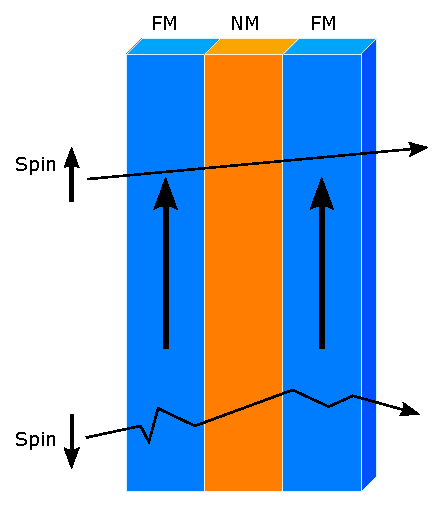
\includegraphics[clip,trim={0mm 0mm 0mm 0mm}, scale=.6]{Ressourcen/IMG/Spin-valve-GMRparallel.eps}
		\caption{Spins in the ferromagnets are parallel, therefore the specific resistance for an electron with the same spin sign can pass the stack easily.}
		\label{fig:nano:GMR:parallel}
	\end{subfigure}
	\hfil
	\begin{subfigure}[r]{0.49\linewidth} 
		\centering
		\includegraphics[clip,trim={0mm 0mm 0mm 0mm},scale=.6]{Ressourcen/IMG/Spin-valve-GMRanti.eps}
		\caption{Spins in the ferromagnets are anti-parallel, every electron has a high scattering probability at one FM-NM interface.}
		\label{fig:nano:GMR:anti}
	\end{subfigure}
	\vfil
	\begin{subfigure}[l]{0.49\linewidth} 
		\centering
		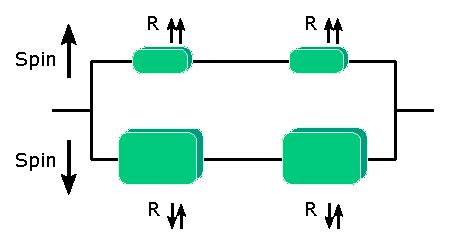
\includegraphics[clip,trim={0mm 0mm 0mm 0mm}, scale=.6]{Ressourcen/IMG/Spin-valve-Rparallel.eps}
		\caption{Resistance model after Campbell and Fert, low specific resistance for up-spin}
		\label{fig:nano:R:parallel}
	\end{subfigure}
	\hfill
	\begin{subfigure}[r]{0.49\linewidth} 
		\centering
		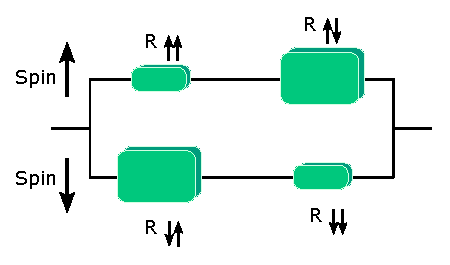
\includegraphics[clip,trim={0mm 0mm 0mm 0mm},scale=.6]{Ressourcen/IMG/Spin-valve-Ranti.eps}
		\caption{Resistance model after Campbell and Fert, medium specific resistance for both spins}
		\label{fig:nano:R:anti}
	\end{subfigure}
	\caption{Spin scattering probability for an arbitrary GMR stack with two Ferromagnets (FM) and a non-magnetic center (NM) after the Mott model. Below a resistance equivalent circuit after the Campbell and Fert model. For increasing scattering at either interface the resulting resistance grows. As in (\protect\subref{fig:nano:GMR:parallel}) and (\protect\subref{fig:nano:R:parallel}) depicted, a spin equal to the spins in a parallelized GMR leads to a very high conductance, whereas a spin anti-parallel to the GMR lowers the conductance dramatically. Nevertheless, the left GMR configuration has the minimal overall resistance. In contrast, the sensor in (\protect\subref{fig:nano:GMR:anti}) and (\protect\subref{fig:nano:R:anti}) achieves the highest possible resistance due to a minimal mean free path length for majority and minority charge carriers.}
	\label{fig:nano:GMR}
\end{figure}


\subsection{Spin Valves with Artificial Anti-Ferromagnets}
The plain GMR sensor has been optimized for maximal $\Delta R$ to sense minimal magnetic dipoles. This was reached by the coupling of a natural anti-ferromagnet to an \acrfull{abbr:aaf}. In strongly patterned materials, anti-ferromagnetism can be observed, when every spin has an alternating counterpart. 
\newpage
This lets vanish the external magnetization, where in the inside two oppositely oriented directions dominate. This is crucial for "pinning" the magnetization axis of a ferromagnet (FM) to the invariant anti-ferromagnet (AFM) axis.\cite{lit:nano:physicsmagneticmaterials} There exist some naturally anti-ferromagnetic materials, but it is state of the art to couple two ferromagnetic nanolayers by the interaction of their neighboring spins via delocalized electrons. Divided by a thin neutral layer, this anti-magnetic stack is mentioned as interlayer exchange coupled artificial \acrshort{abbr:afm}.\cite{lit:nano:spinelectronics}\\ As advantage over the simple Spin Valve, the hardness of the reference layer is enhanced, because the \acrshort{abbr:aaf} exhibits extremely few magnetic momentum to the outside and can hardly be changed by an external field. This system is also used to refine the unidirectional anisotropy of the reference layers.\cite{patent:wheatstone_GMR} As further improvement measure, an insulating oxide was sputtered on top of the free layer to reflect electrons spin preserving into the active zone. 
\newpage

\begin{figure}[h]
	\centering
	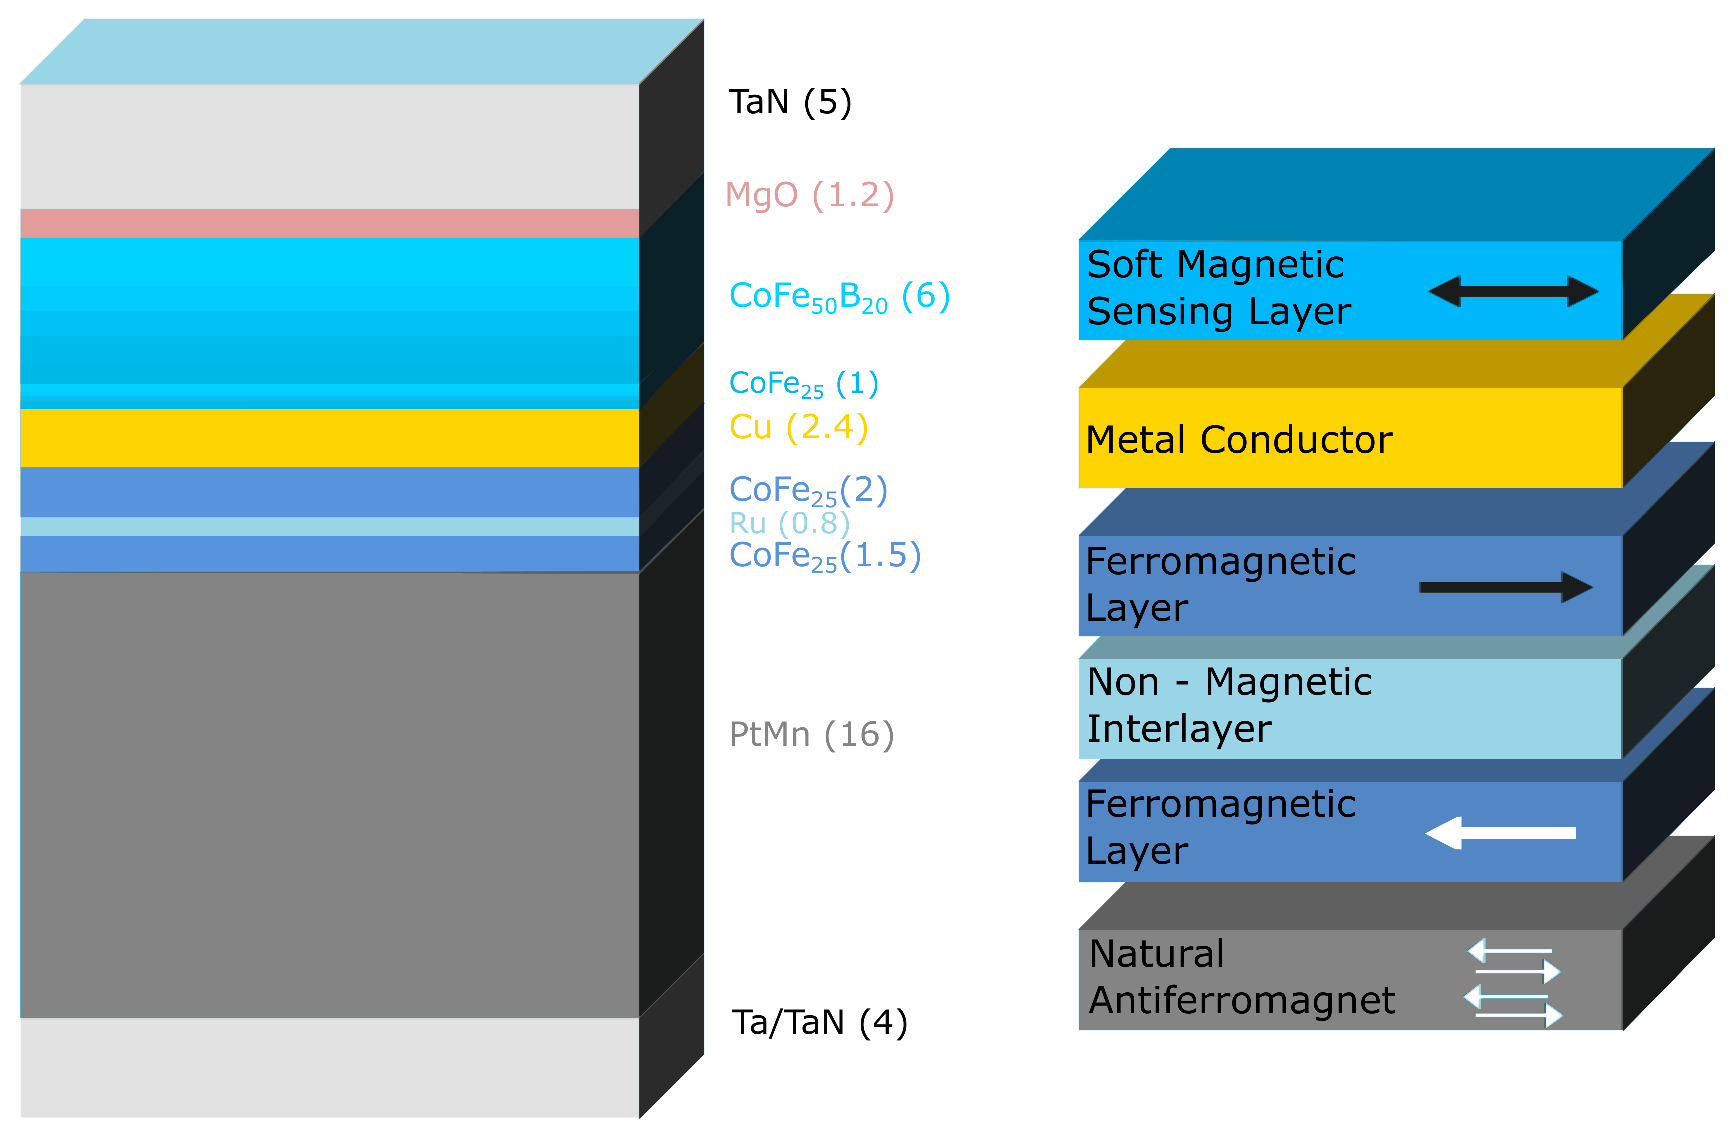
\includegraphics[scale=.5]{Ressourcen/IMG/GMR-Stack-with-text}
	\caption{A typical Siemens-GMR sensor stack depicted with its molecular sputter compounds and layer thicknesses [nm] is shown on the left side. Between the passivation layers of TaN is the magnetic configuration stashed as drawn on the right side with an anti-ferromagnet coupled to an artificial anti-ferromagnet above. The top magnetically hard layer acts as the reference for the soft magnetic sensing stack separated by a metal conductor to avoid magnetic coupling. Maximizing the GMR-sensitivity, a thin MgO layer is applied to the upside, which reflects charge carriers without altering the spin polarization \cite{lit:Helou}}
	\label{fig:nano:gmr-stack}
\end{figure}

The GMR fabrication process involved multilayer lithography and sputtering to stack different materials. After the etching procedure, electron spins were aligned to each other by Field-Cooling, which heats the materials over the N\'{e}el - Relaxation Temperature (Eq. \ref{eq:nano:neel-arrhenius}) and lets them cool down at a defined magnetic field. On the bottom and top tantalum-mono-nitride (4-\SI{5}{\nano\meter}) is deposited as a adhesion enhancement and further passivation of the stack against external influences. Platinum manganese (\SI{16}{\nano\meter}) is a commonly used anti-ferromagnet, whose inner anti-parallel magnetization generates an net zero magnetic momentum to the outside.\\
Under heating, a magnetically hard CoFe$_{25}$ layer(\SI{1.5}{\nano\meter}) is pinned to the anti-ferromagnet. To couple the reference layer of cobalt alloy (\SI{2}{\nano\meter}) - anti-parallel magnetized - to the one below, a thin rubidium film (\SI{0.8}{\nano\meter}) is applied for exploiting the oscillating indirect exchange interaction. This configuration serves as an \acrshort{abbr:aaf}, which is insensitive to external magnetic fields. On top of that, the sensing layer made out of the magnetically soft material CoFe$_{40}$B$_{20}$ (\SIrange{3}{6}{\nano\meter}) over a decoupling, conducting copper structure (\SI{2.4}{\nano\meter}).

There were different dimensions for the sensing layer evaluated, because a thinner version could yield more sensitivity although the relative change in resistance (Eq. \ref{eq:nano:resistance_rel_change}) would decrease (Table \ref{tab:gmr:layer_sensitivity}). For amplifying this resulting resistance CoFe$_{25}$ (\SI{1}{\nano\meter}) is applied below. Furthermore, MgO (\SI{1.2}{\nano\meter}) is sputtered on the top side to reflect charges without loosing their spin-polarization.\cite{lit:Helou}
%
\begin{table}[htb!]
	\centering
	\begin{tabularx}{\linewidth}{|C|c|c|c|c|c|c|c|}
		\hline 
		\textbf{Freelayer} & \textbf{Sensitivity}	& $\frac{\frac{\mathbf{mV}}{\mathbf{V}}}{\mathbf{mT}}$ & \textbf{H$_e$} [\si{\ampere\per\meter}] & \textbf{B$_e$} [\si{\milli\tesla}] & \textbf{H$_c$} [\si{\ampere\per\meter}]   & \textbf{ B$_e$} [\si{\milli\tesla}] & $\mathbf{\frac{\Delta R}{R}}$ [\si{\percent}]\\ 
		\hline 
		5 nm & 16.15& 1.00 &  0.06 & 0.15 & 0.03  & 0.01 & 11.5\\ 
		\hline 
		3 nm &29.21& 2.50 & 0.91 & 0.08 & 0.20  & 0.06 &  11.0\\ 
		\hline 
	\end{tabularx} 
	\caption{Sensitivity of one 2 x \SI{30}{\micro\meter} GMR in relation to the free layer thickness. Sensitivity can be significantly increased by lowering the thickness of the soft magnetic material.}
	\label{tab:gmr:layer_sensitivity}
\end{table}
\newpage
\section{Droplet Microfluidics}
"Microfluidics is both the science, which studies the behavior of fluids through micro-channels, and the technology of manufacturing microminiaturized devices containing chambers and tunnels through which fluid and flow are confined.
Microfluidics deal with very small volumes of fluids, down to femtoliters [...]."\cite{lit:nano:eveflow} As new areas of this field are still investigated, there is an increasing demand for theoretical and experimental work on fluid mechanics at this scale. In order to determine the right concept for the microchannels' layout and properties, some well-defined guiding values can be examined.
\begin{figure}[htb]
	\includegraphics[clip,width=\linewidth,trim={0mm 0mm 0mm 11mm}]{Ressourcen/IMG/Steady_state}
	\caption{Microfluidic T-junction with two phases, oil from the right and water from the top connection at low Reynolds number.}
	\label{fig:fluidics:steady-state}
\end{figure}

To determine if the desired laminar flow is existent in the fluidic, it is common practice to evaluate the Reynolds number $\mathbf{Re}$ and compare it to the critical transition value of 2000.\cite{lit:fluidic:microfluidics_review} This number describes the ratio between inertial and viscous forces (Eq. \ref{eq:fluidics:Re}), with $\rho$ as the density of medium, the characteristic velocity $u_c$, the characteristic length $l_c$ and the dynamic viscosity $\eta$. These characteristic values represent a typical length scale in the effective area of the inertial or viscous forces, which are in this case fluid velocities up to \SI{1}{\centi\meter\per\second} and lengths up to \SI{50}{\micro\meter} maximal diameter. Solving the equation with the boundary of Hagen-Poiseuille flow profiles and for an aqueous fluid, one gets Reynolds Numbers up to $\mathcal{O}(1)$ after the Landau notation and has safely laminar flow in the channels, that can be observed in figure \ref{fig:fluidics:steady-state}.
\begin{align}
 \mathrm{Reynolds\ Number}\ \mathbf{Re} &= \frac{\rho u_c  l_c}{\eta}
 \label{eq:fluidics:Re}\\
  \mathrm{P\acute{e}chlet\ Number}\ \mathbf{Pe} &= \frac{u_c l_c}{D}
 \label{eq:fluidics:Pe}\\
 \mathrm{Capillary\ Number}\ \mathbf{Ca} &= \frac{\mu u_c}{\sigma}
 \label{eq:fluidics:Ca}
\end{align}
Only partially interesting was the convection to diffusion ratio, described through the P\'{e}chlet number (Eq. \ref{eq:fluidics:Pe}), which was mattering in this way, that diffusion of the nanoparticles in the fluid is far slower than the experiment's duration, thus can be neglected.

However, the dimensionless Capillary number $\mathbf{Ca}$ (Eq. \ref{eq:fluidics:Ca}) is a crucial parameter to gather information about the balance between interfacial and viscous stresses. This is particularly interesting for the formation of microfluidic droplets with two immiscible fluids, where these two stresses drive the system; surface tension tries to reduce the interfacial area, while viscous forces act to extend and drag the interface downstream.\cite{lit:fluidic:microfluidics_review}

Emulsions are a crucial factor in materials and food with a wide range of applications. Conventional emulsification processes such as shaking or ultrasonic excitation generate still inhomogeneous and polydisperse droplets with large diameters. Recently, the growing trends in miniaturization of experimental systems have pushed the droplet-based applications from traditional emulsions to microanalysis, drug delivery and chemical microreactions.\\
Monodisperse droplets have been produced by many different methods: geometry dominated breakup, cross flows, perpendicular flow-induced breakup and hydrodynamic flow focusing. Despite the advances in the past time, major challenges still are the quantization of flow rates, viscosities and the channel wetting ability of the fluids. \cite{lit:fluidics:monodisperseDroplets}

\subsubsection{T-Junction}
One of the most common geometry for a droplet generator invented by \citet{lit:fluidics:t-junction:first}, has been the so called T-junction.(Fig. \ref{fig:fluidics:steady-state}) It is designed, to form an intersection between a dispersed phase microchannel, usually filled with aqueous solution, and a perpendicular main channel, which contains the continuous phase - in most cases oil. The continuous phase then causes forces upon the water solution that periodically break up droplets into the main channel.\cite{lit:fluidics:droplet:formation:t-junction:transition_exp} 

In droplet formation generally exist three regimes: squeezing, a regime at low Capillary numbers, dripping, a regime with moderate Capillary numbers, and jetting, a regime at high Reynolds and Capillary numbers. In between these ranges lay instable transitional domains, which also vary at $\mathbf{Re}$ and $\mathbf{Ca}$. The flow rates, which these dimensionless numbers underlie indirectly, can then determine the operating range of the system.

\begin{figure}[htb]
	\begin{subfigure}{0.49\linewidth}
		\centering
		\includegraphics[page=2,clip,trim={60mm 160mm 00mm 20mm},width=\linewidth]{Ressourcen/PinchOff/Droplet_Formation}
		\caption{Intrusion}
		\label{fig:fluidics:droplet:dripping:intrusion}
	\end{subfigure}
	\hfil
	\begin{subfigure}{0.49\linewidth}
		\centering
		\includegraphics[page=4,clip,trim={60mm 160mm 00mm 20mm},width=\linewidth]{Ressourcen/PinchOff/Droplet_Formation}
		\caption{Blocking}
		\label{fig:fluidics:droplet:dripping:blocking}
	\end{subfigure}
	\vfil
	\begin{subfigure}{0.49\linewidth}
		\centering
		\includegraphics[page=6,clip,trim={60mm 160mm 00mm 20mm},width=\linewidth]{Ressourcen/PinchOff/Droplet_Formation}
		\caption{Pinch-off}
		\label{fig:fluidics:droplet:dripping:pinchoff}
	\end{subfigure}
	\hfil
	\begin{subfigure}{0.49\linewidth}
		\centering
		\includegraphics[page=8,clip,trim={60mm 160mm 00mm 20mm},width=\linewidth]{Ressourcen/PinchOff/Droplet_Formation}
		\caption{Breakup}
		\label{fig:fluidics:droplet:dripping:breakup}
	\end{subfigure}
	
	\caption{Typical droplet formation at a T-junction in the \textbf{dripping regime} with two phases (continuous:oil, dispersed: water). At first the pressure pushes the tip of the fluid into the main channel(\SI{70}{\micro\meter}) without any interaction.(\protect\subref{fig:fluidics:droplet:dripping:intrusion}) When the pressure on the right side builds up due to the blocking of a considerable channel width, the droplet begins to deform in flow direction.(\protect\subref{fig:fluidics:droplet:dripping:blocking}) Eventually, this action continues until a critical neck diameter is reached and the droplet detaches.(\protect \subref{fig:fluidics:droplet:dripping:pinchoff}) The upstream pressure drops very quickly and the drop is accelerated towards the channel center.(\protect\subref{fig:fluidics:droplet:dripping:breakup})}
	\label{fig:fluidics:droplet:dripping}
\end{figure}

For a flow ratio $\delta = \frac{Q_c}{Q_d}$ much smaller than one, dripping occurs uniquely caused by shear stress. There, the viscous force rips the continuous phase apart after it overcame the interfacial tension, when it protrudes into the channel. (Fig.\ref{fig:fluidics:droplet:dripping})

A $\delta$ within the order of 1 in combination with a low Capillary number induces the squeezing regime. There the shear stress only deforms the in-streaming phase, while the interfacial tension acts against a droplet formation. When the emerging interface fills the junction, pressure starts to build up upstream. This excess pressure squeezes the neck of a plug and facilitates its pinch-off.\cite{lit:fluidics:droplet:formation:transition} Plug is the term for a non-spheroid droplet, which is deformed, because the channel width is smaller than its undeformed diameter. As the hydraulic resistance increases dramatically with the cubic of the channel intersection area, the continuous phase will be detached eventually and the overpressure cause a distance between two plugs.\cite{lit:fluidics:BioMEMS}

\begin{figure}[h!]
	\begin{subfigure}{0.249\linewidth}
		\centering
		\includegraphics[page=4,clip,trim={10mm 190mm 00mm 20mm},width=\linewidth]{Ressourcen/PinchOff/Squeezing}
		\caption{Intrusion}
		\label{fig:fluidics:droplet:squeezing:intrusion}
	\end{subfigure}
	\hfil
	\begin{subfigure}{0.24\linewidth}
		\centering
		\includegraphics[page=8,clip,trim={10mm 190mm 00mm 20mm},width=\linewidth]{Ressourcen/PinchOff/Squeezing}
		\caption{Blocking}
		\label{fig:fluidics:droplet:squeezing:blocking}
	\end{subfigure}
	\hfil
	\begin{subfigure}{0.24\linewidth}
		\centering
		\includegraphics[page=12,clip,trim={10mm 190mm 00mm 20mm},width=\linewidth]{Ressourcen/PinchOff/Squeezing}
		\caption{Pinch-off}
		\label{fig:fluidics:droplet:squeezing:pinchoff}
	\end{subfigure}
	\hfil
	\begin{subfigure}{0.24\linewidth}
		\centering
		\includegraphics[page=13,clip,trim={10mm 190mm 00mm 20mm},width=\linewidth]{Ressourcen/PinchOff/Squeezing}
		\caption{Breakup}
		\label{fig:fluidics:droplet:squeezing:breakup}
	\end{subfigure}
	
	\caption{Typical droplet formation at a T-junction in the \textbf{squeezing regime} with two phases (continuous:oil, dispersed: water). At first, the dispersed fluid fills the main channel(\SI{70}{\micro\meter}).(\protect\subref{fig:fluidics:droplet:squeezing:intrusion}) While the channel is obstructed, the pressure on the upstream side builds up.(\protect\subref{fig:fluidics:droplet:squeezing:blocking}) Eventually, this overpressure continues to form a necking at the junction wall until a critical diameter is reached and the plug detaches.(\protect \subref{fig:fluidics:droplet:squeezing:pinchoff}) The upstream pressure drops very quickly and the plug is accelerated towards the channel outlet.(\protect\subref{fig:fluidics:droplet:squeezing:breakup})}
	\label{fig:fluidics:droplet:squeezing}
\end{figure}

The jetting regime will be only shortly covered, because it falls into an undesired case of this work. Jetting occurs, where the flow ratio $\delta \gg 1$ and also at higher Capillary numbers, because of low interfacial tensions. Being in this regime, the stream of the dispersed fluid extends downstream
of the T-junction and the two immiscible phases are in laminar flow side-by-side over
lengths of the channel, which are at least several times larger than its width, caused by the inertial effects of the dispersed phase.\cite{lit:fluidics:droplet:formation:jetting}


\subsubsection{Y- and Cross-Junctions}
\begin{wrapfigure}[6]{r}{0.55\linewidth}
	\vspace{-5mm}
	\begin{subfigure}{0.49\linewidth}
		\centering
		\includegraphics[clip,trim={0mm 0mm 5mm 15mm}, width=.9\linewidth]{Ressourcen/IMG/y-junction}
		\caption{Y-junction}
		\label{fig:fluidics:droplet:y-junction}
	\end{subfigure}
	\hfil
	\begin{subfigure}{0.49\linewidth}
		\centering
		\includegraphics[clip,trim={0mm -3mm 00mm 15mm},width=1.1\linewidth]{Ressourcen/IMG/cross-junction}
		\caption{Cross-junction}
		\label{fig:fluidics:droplet:cross-junction}
	\end{subfigure}
	
	\caption{Droplet formation in different channel geometries, mainly via viscous forces in (\protect\subref{fig:fluidics:droplet:y-junction}) and mainly via shear forces in (\protect \subref{fig:fluidics:droplet:cross-junction})}
	\label{fig:fluidics:droplet:junctions}
\end{wrapfigure}

Besides the T-junction, there exist various other channel geometries for different purposes and applications. Derived from the original T-shape, the Y-junction has also been widely established. The same regimes can there be reached as well as the droplet diameters, while having two equally wide inlet channels. The advantage over the T-junction thereby is a higher sensitivity to the viscosity ratio in dependence on the angle between both inlets.\cite{lit:fluidic:microfluidics_review}\\
Similarly, the cross-junction consists of one bigger main channel and two perpendicular with the same width, which carry the continuous phase. At the moment, there exist only few experimental evaluations of this geometry, but the dripping and squeezing regimes have already been confirmed. Squeezing into the continuous flow from the top, mainly plug droplets are produced, where the dispersed phase blocks the lateral flows. The squeezed thread begins to thin down quasi-statically through
the effect of the hydrodynamic forcing.\cite{lit:fluidics:droplet:dynamics} Pinch-off and breakup at the junction or its immediate vicinity are then governed by the formerly mentioned viscous and interfacial stresses. In the dripping regime, the droplet's width is smaller or close to the main channel's orifice as the dispersed phase protrudes and retracts continuously.\cite{lit:fluidics:droplet:formation:cross:squeezing}
\clearpage
\newpage\null\thispagestyle{empty}\newpage
\chapter{Materials and Methods}
\section{GMR Sensor Fabrication and Characterization}
The GMR sensor was designed after the first Siemens-GMR  in 1999.\cite{patent:GMR} These ready-to-use silicon chips with dimensions of 20 x \SI{10}{\milli\meter} were manufactured by Sensitec GmbH after a mask template.  Multiple heaps and their guiding structures were placed on \SI{6}{\inch}-wafers, passivated with \SIlist{70;100;200}{\nano\meter} of silicon nitride to withstand corrosiveness of the ionic \acrfull{abbr:pbs}. In the center of each chip, six sensor elements were arranged as Wheatstone half bridges with distances varying from \SIrange{10}{22}{\micro\meter}. The sensor was manually attached inside a rectangular hole of a Printed Circuit Board (Piu-Printex GmbH) on a glass piece covered with double-side tape. The connection between silicon and the electrical wires on the \acrfull{abbr:pcb} is achieved via thermo-sonic wedge-wedge bonding (HB10, TPT Wire Bonder GmbH \& CoKG). A variable combination of ultrasound, the resulting heat and mechanical pressure (\SI{280}{c\newton\meter}) of a conical tool fixes in \SI{100}{\milli\second} a \SI{25}{\micro\meter} thick copper-alloy-wire (Cu-HC4) on a \SI{200}{\nano\meter} thick aluminum - bond pad on the chip (\SI{220}{\watt}) and on a 300 x \SI{300}{\micro\meter\square} gold - bond pad at the printed circuit board (\SI{320}{\watt}). The wires on the PCB are connected to conducting through-bores. A 48-pin socket-plug connector (TE Connectivity DIN 41612, RS Components) was soldered onto the backside for connection to a readout electronics circuit.
\newpage
\subsection*{GMR Characterization}
The Spin-Valve can be evaluated by its hysteresis due to a change in an external magnetic field. For that, two Helmholtz coils were positioned around the sensor, generating $\pm$\SI{15.6}{\milli\tesla} homogeneously and orthogonal to the easy axis of the GMR. These are driven by a voltage controlled power supply (BOP 50-8M, Kepco Inc.) with $\pm$ \SI{2}{\ampere} at \SI{20}{\volt} peak-to-peak.
\begin{figure}[!h]
	\includegraphics[scale=.49, trim=90 0 0 0]{Ressourcen/IMG/Hysteresis_plot_S60C7}
		\centering
	\caption{Hystereses during the alignment of a NdFeB - magnet below a GMR half bridge. The slope in the zero-crossing (dashed lines) of one hysteresis - shown by the red line - has to be maximized during the spatial positioning of the magnet below. The red crosses, if projected to the x axis, indicate the coercivity field strength of the sensor stack, which displays the magnetic field needed to degauss the GMR after saturation. Due to the fact, that the detector is much fewer actuated by bead aggregations (\si{\micro\tesla}) than by the saturation field at this measurement (\si{\milli\tesla}), the difference in H$_c$ can be neglected.}
	\label{fig:hysteresis}
\end{figure}
\\The current signal of one bridge as a response to a sinusoidal excitation signal at \SI{100}{\milli\volt} and \SI{1}{\kHz} from a frequency generator (33120A, Hewlett-Packard) was fed into an trans-impedance converter (SR570, Stanford Research Systems) and subsequently the voltage signal into a lock-in-amp (LIA-MVD-200-H, Femto Messtechnik GmbH) for a 30-fold analog amplification. \\Then, analog-digital-conversion was reached using a DAQ-PCI card (PCI-6251/USB-6351, NI Corp.) with a sampling rate of \SI{500}{\kHz}. This input was parsed and plotted in LabVIEW environment at the computer.
\newpage
From the hysteresis curve the magnetoresistive effect and the anisotropy field can be derived, which determine the sensitivity of the system (Eq. \ref{eq:nano:resistance_rel_change}). 
The magnetization of the superparamagnetic droplet is achieved with an excitation field generated by a 32 x 27 x \SI{5}{\mm} NdFeB permanent magnet underneath the sensor chip.\\The position of the permanent magnet is then adjusted with respect to the slope of the hysteresis curve.(Figure \ref{fig:hysteresis}) In this way field components of the permanent magnet in the sensor plane are minimized and ensure highest sensitivity for magnetic field detection.\cite{lit:Helou}
\subsection*{Electrical Readout Circuit}
The GMR bridge was supplied at frequencies from \SIrange{20}{50}{\kHz} and at V$_{pp}$ from \SIrange{100}{400}{\mV}. The lock-in captured a differential signal from the Wheatstone bridge and dampened the noise \SI{60}{\dB} (enhanced the signal 30,000x) at a time constant of \SI{300}{\micro\second}, while comparing the measurement signal to the reference signal of the function generator in the manner of a lowpass filter. The resulting DC signal is then digitized with a sample rate of 10 kHz and a bit depth of 16 Bit.\\ Inside the computer, the measurement is sampled at \SI{10}{\kHz}, filtered and plotted continuously with different FIR-filters. At the meantime, a video stream through a camera (TXG14F, Baumer GmbH) mounted on the microscope (DM2500, Leica Microsystems) is played and the plotted data is simultaneously stored on the hard drive in the LabVIEW format ".tdms".
\newpage
\section{Microfluidic Fabrication Process}
\subsection{Mask Designs}
At first, the template for my foil masks (KOENEN GmbH), which where printed on the master of later microfluidics, was drawn in AutoCAD 2019. I tried several designs to fit over the 2 x \SI{30}{\micro\meter\squared} GMR sensor. The in- and outlet diameter was already determined to empirical values of \SI{1.70}{\mm} and also the centered position of the main channel inside the \acrfull{abbr:pdms} slice, while the dimensions free to choose were the channel width and the junction properties. As a first approach, the commonly used perpendicular T-junction was drawn at different channel widths.

Discussed in multiple papers, the channel width ratio $\lambda = \frac{W_{dispersed}}{W_{continuous}}$ depends on the Capillary Number $\mathbf{Ca}$ (Eq. \ref{eq:fluidics:Ca}) if you want to achieve plug formation.\cite{lit:fluidics:droplet:formation:t-junction:squeezing_dripping}\cite{lit:fluidics:droplet:formation:t-junction:numerical}
\begin{align}
\mathbf{Ca}_{oil} & = \frac{\eta_{oil}\ u_c}{\sigma_{Water,Oil}} = \frac{\SI{13.8}{\milli\pascal\second}\ \cdot\ \SI{10}{\milli\meter\per\second}}{\SI{35.26}{\milli\newton\per\m}} = \SI{3.91e-3}{}
\label{eq:fluidics:Ca:oil}\\	
\mathbf{Ca}_{PBS} &= \frac{\eta_{PBS}\ u_c}{\sigma_{Water,Oil}} = \frac{\SI{1.05}{\milli\pascal\second}\ \cdot\ \SI{10}{\milli\meter\per\second}}{\SI{35.26}{\milli\newton\per\m}} = \SI{2.98e-4}{} 	\label{eq:fluidics:Ca:PBS}
\\\mathbf{Ca}_{oil+2\%Span} & = \frac{\eta_{oil+2\%Span}\ u_c}{\sigma_{Water,Oil}} =
\begin{cases} \mbox{\SI{9.50e-3}{\milli\pascal\second},} & \mbox{}\eta_{oil+2\%Span} = \SI{33.5}{\milli\pascal\second} \\ \mbox{\SI{1.23e-2}{\milli\pascal\second},} & \mbox{} \eta_{oil+2\%Span} = \SI{43.5}{\milli\pascal\second} \end{cases}\label{eq:fluidics:Ca:oil+span}
\end{align}
 The chair couldn't measure the interfacial tension of the PBS and mineral oil phase by themselves, so a very similar experimental value described by \citet{lit:fluidics:interf_tension_oil_water} was used. The temperature dependent regression line $\sigma_{Water,Oil} =  0.122T + 32.82$ gave a surface tension \SI{35.26}{\milli\newton\per\m} at \SI{20}{\degreeCelsius} room temperature. 
 \newpage
 Taking into consideration that the oil has been mixed with \SI{2}{\percent} Span80 beforehand, the dynamic viscosity $\eta_{oil+2\%Span}$ should reach viscosities between \SIrange{33.5}{43.5}{\milli\pascal\second} assuming linear dependency. The Capillary numbers then resulted at a desired 
 \begin{wrapfigure}[8]{r}{.5\linewidth}
		\centering
		
\includegraphics[trim={0mm 0mm 0mm 1mm},width=\linewidth]{Ressourcen/AutoCAD/T_junction_round_zoomed}
		\caption{Optimized non-perpendicular T-junction layout for an enhanced droplet generation}
		\label{fig:CAD:t-junction-zoomed}	
\end{wrapfigure}
characteristic velocity $\mathbf{u_c}$ = \SI{1}{\centi\meter\per\second} (for a sufficient distance between the measured signal peaks) to values in equations \ref{eq:fluidics:Ca:oil}, \ref{eq:fluidics:Ca:PBS} and \ref{eq:fluidics:Ca:oil+span}. 
These small Capillary numbers are desired, because they permit a stable and continuous plug flow, when the interfacial force dominates the shear force. For these values, \citet{lit:fluidics:droplet:formation:t-junction:numerical} showed that a channel width ratio less than unity is more favorable. Therefore, a design with a $\lambda = \frac{2}{3}$ seemed to satisfy this condition. This was implemented on T-junctions starting at 30:\SI{20}{\micro\meter} to 100:\SI{66.7}{\micro\meter}.(Figure \ref{fig:CAD:t:perp})


Another approach has been an optimized version of this T-junction similar to droplet generators of Elveflow.\cite{lit:nano:eveflow} This geometry with a necking on the opposite site of the perpendicular junction inlet (Figure \ref{fig:CAD:t:round}) tries to force a more homogeneous and reproducible droplet pinch-off than standard geometries due to a higher pressure in between the critical pinch-off and breakup area.


	\begin{figure}[h]
			\centering
			\subcaptionbox{3:2 - T-Junction with perpendicular connection \label{fig:CAD:t:perp}}[0.49\linewidth]{
			\includegraphics[clip,trim={50mm 5mm 0mm 40mm},scale=.30]{Ressourcen/IMG/Microfluidics_Prototype_3_2018412-t_Junction_perp}
			}
		\hfil
			\subcaptionbox{3:2 - T-Junction with an adapted connection \label{fig:CAD:t:round}}[0.49\linewidth]{
		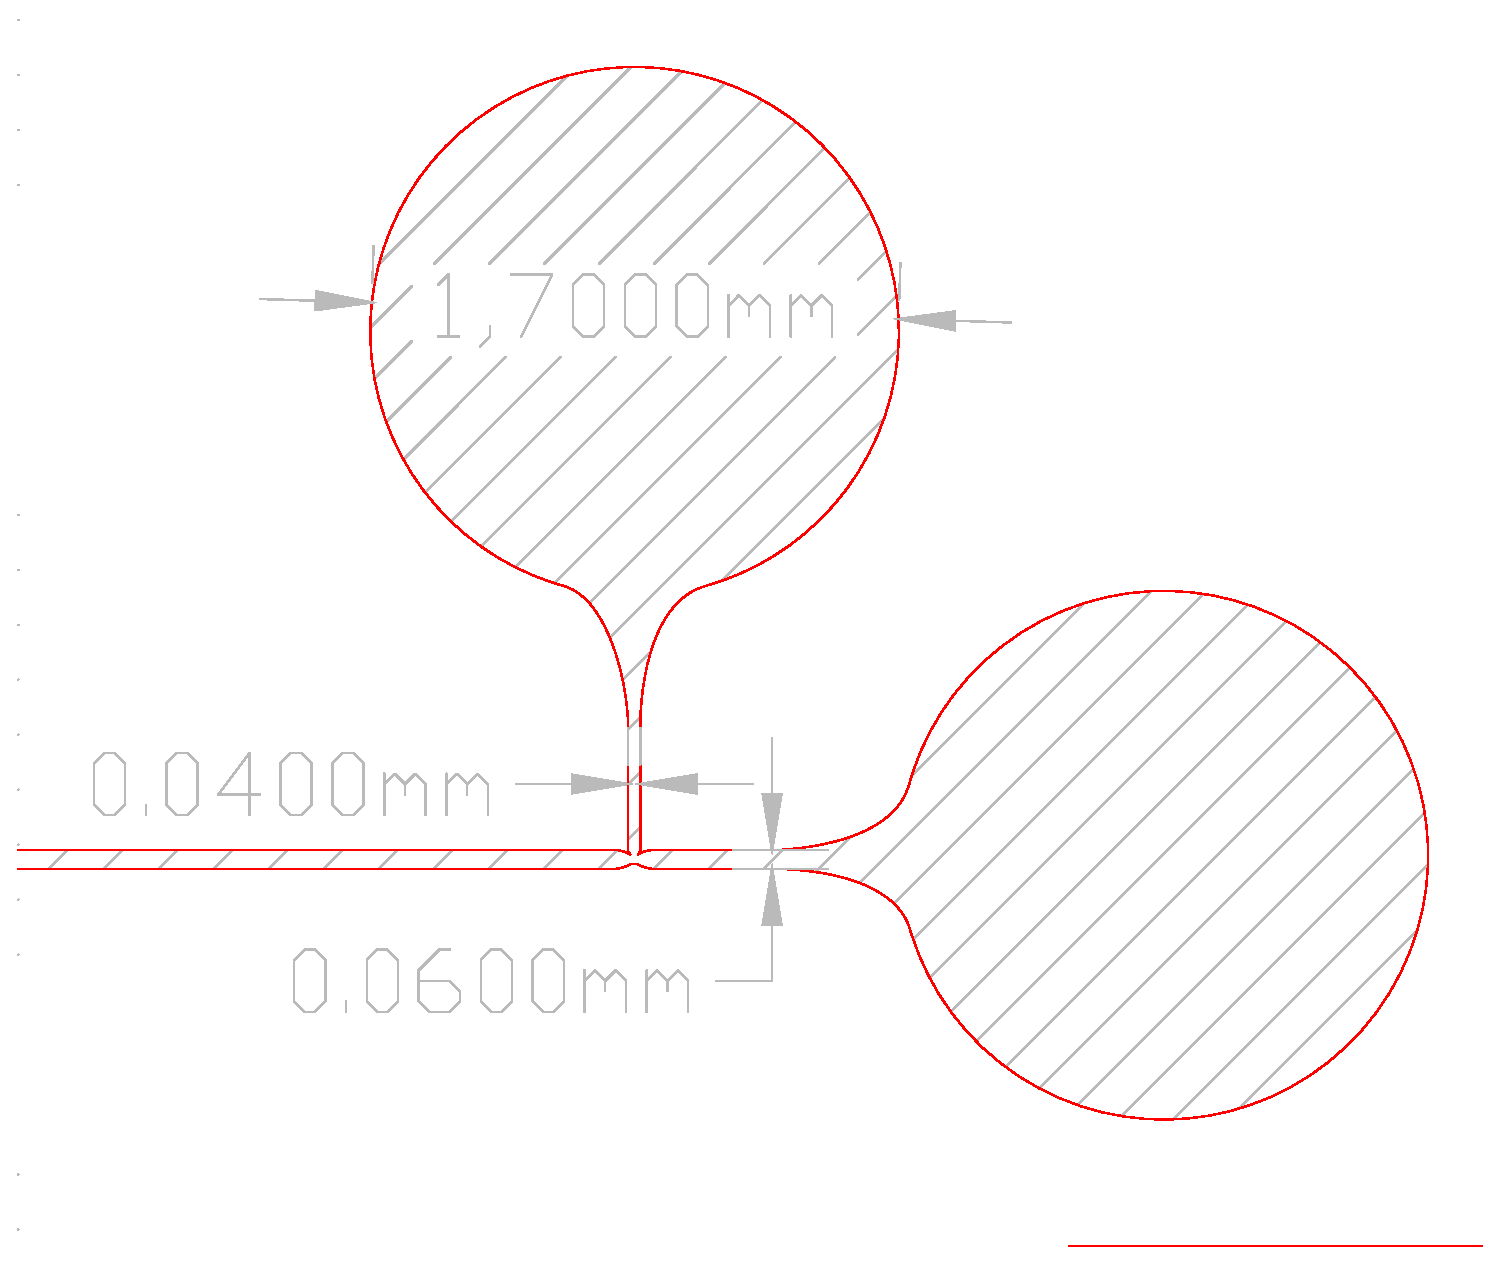
\includegraphics[clip,trim={10mm 10mm 0mm 0mm},scale=.3]{Ressourcen/AutoCAD/T-junction_complete_round}
		}
\caption{T-junction designs with perpendicular (\protect\subref{fig:CAD:t:perp}) and smoothed connection after an injection model to facilitate the droplet pinch-off in the squeezing regime with a higher local pressure (\protect\subref{fig:CAD:t:round}). The main channel width (\textasciitilde desired droplet width) is \SI{60}{\micro\meter}, while the perpendicular channel is \SI{40}{\micro\meter} wide.}
\label{fig:CAD:t}
\end{figure}
\newpage

\begin{figure}[h]
	\begin{subfigure}[l]{0.49\textwidth} 
		\centering
		\includegraphics[clip,trim={0mm 0mm 0mm 0mm}, scale=.22]{Ressourcen/IMG/Microfluidics_Prototype_3_2018412-Cross-junction2}
		\caption{3:2:2 - cross-junction design with two inlets}
		\label{fig:CAD:cross:2IN}
	\end{subfigure}
	\hfil
	\begin{subfigure}[r]{0.49\textwidth} 
		\centering
		\includegraphics[clip,trim={0mm 0mm 0mm 0mm},scale=.22]{Ressourcen/IMG/Microfluidics_Prototype_3_2018412-Cross-junction3}
		\caption{3:2:2 - cross-junction design with three inlets}
		\label{fig:CAD:cross:3IN}
	\end{subfigure}
	\caption{Cross-junction design for droplet formation, the inlets perpendicular to the main channel are each $2/3$ of the main channel width. A design with one inlet for continuous and dispersed phase (\protect\subref{fig:CAD:cross:2IN}) was chosen to facilitate the fabrication process. The design with three inlets (\protect\subref{fig:CAD:cross:3IN}) was evaluated as a double T-junction or with the possible application of two continuous phases.}
\end{figure}
In contrast to the T-junction, a cross-flow device was also constructed after the same specifications. We assumed to get a more precise and predictable system for various plug lengths.  On the one hand side a device geometry was designed with only two inlets for three channels (Fig. \ref{fig:CAD:cross:2IN}), where the continuous phase would split into two for easier fabrication and an ensures equal flow rate inside both canals. On the other hand side, I chose a three inlet dimensionality (Fig. \ref{fig:CAD:cross:3IN}) to let either two continuous or dispersed phases flow in a cross flow or double T-junction configuration. Another advantage over the 2-In geometry is also, that syringe pump inaccuracy can be averaged out. The both cross-junctions were also implemented accordingly to the design rules of the T-junction.

The above discussed concepts were realized in two different manners. We designed one mask exclusively for tests of the suitable geometry, dimensions and evaluation of right syringe pump parameters.(Fig. \ref{fig:CAD:mask:single}, \ref{fig:CAD:mask:test}) The smoothed T-junction and both cross-junctions each received a single mask with different channel widths, which was developed for a later positioning in the PCB with the GMR-sensors.
\begin{figure}[h!]
	\vspace{-2cm}
	\begin{subfigure}[c]{\textwidth}
		\centering
		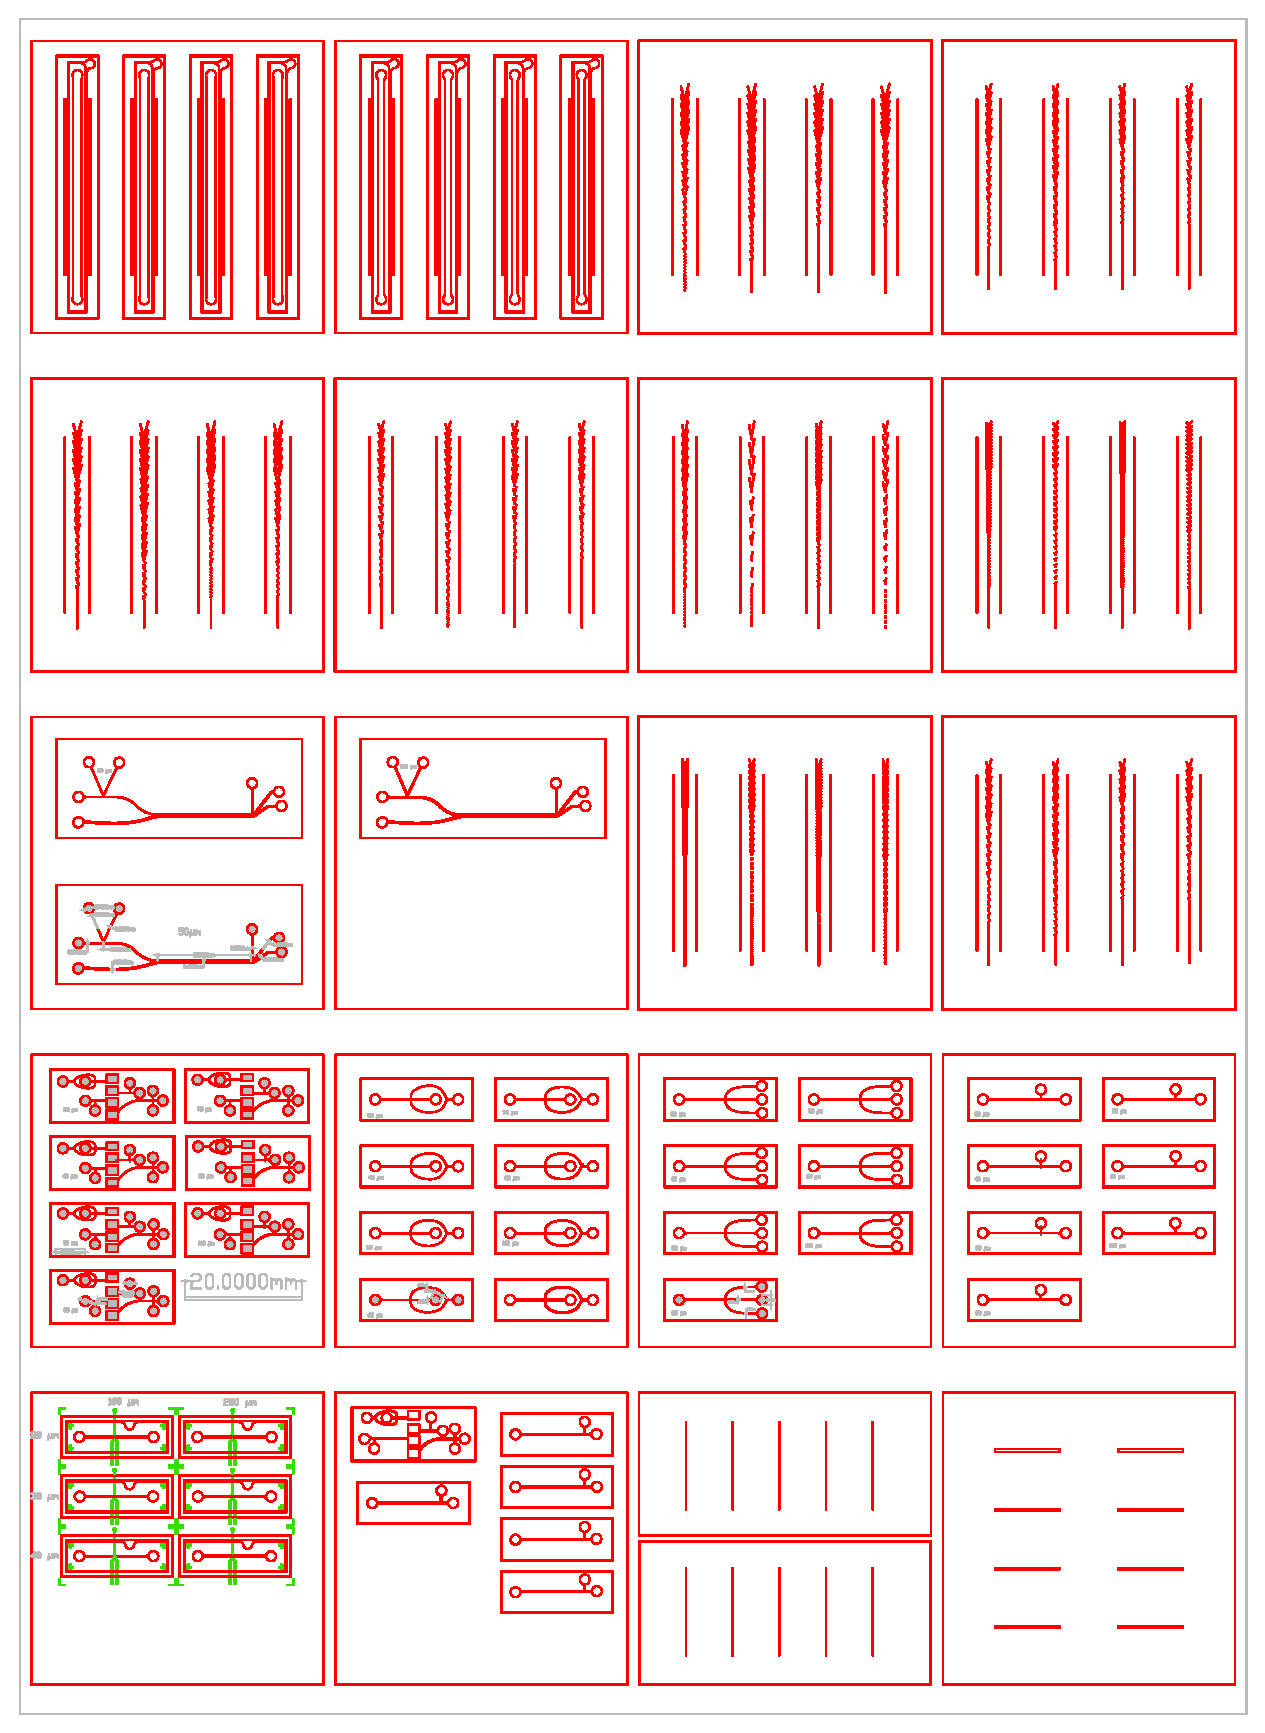
\includegraphics[clip,trim={0mm 0mm 0mm 0mm},scale=.3]{Ressourcen/IMG/Microfluidics_Prototype_3_2018412-A4}
		\caption{Complete DIN-A4 mask layout different microfluidic structures}
		\label{fig:CAD:mask:A4}
	\end{subfigure}
	\vfill
	\begin{subfigure}[c]{\textwidth}
		\centering
		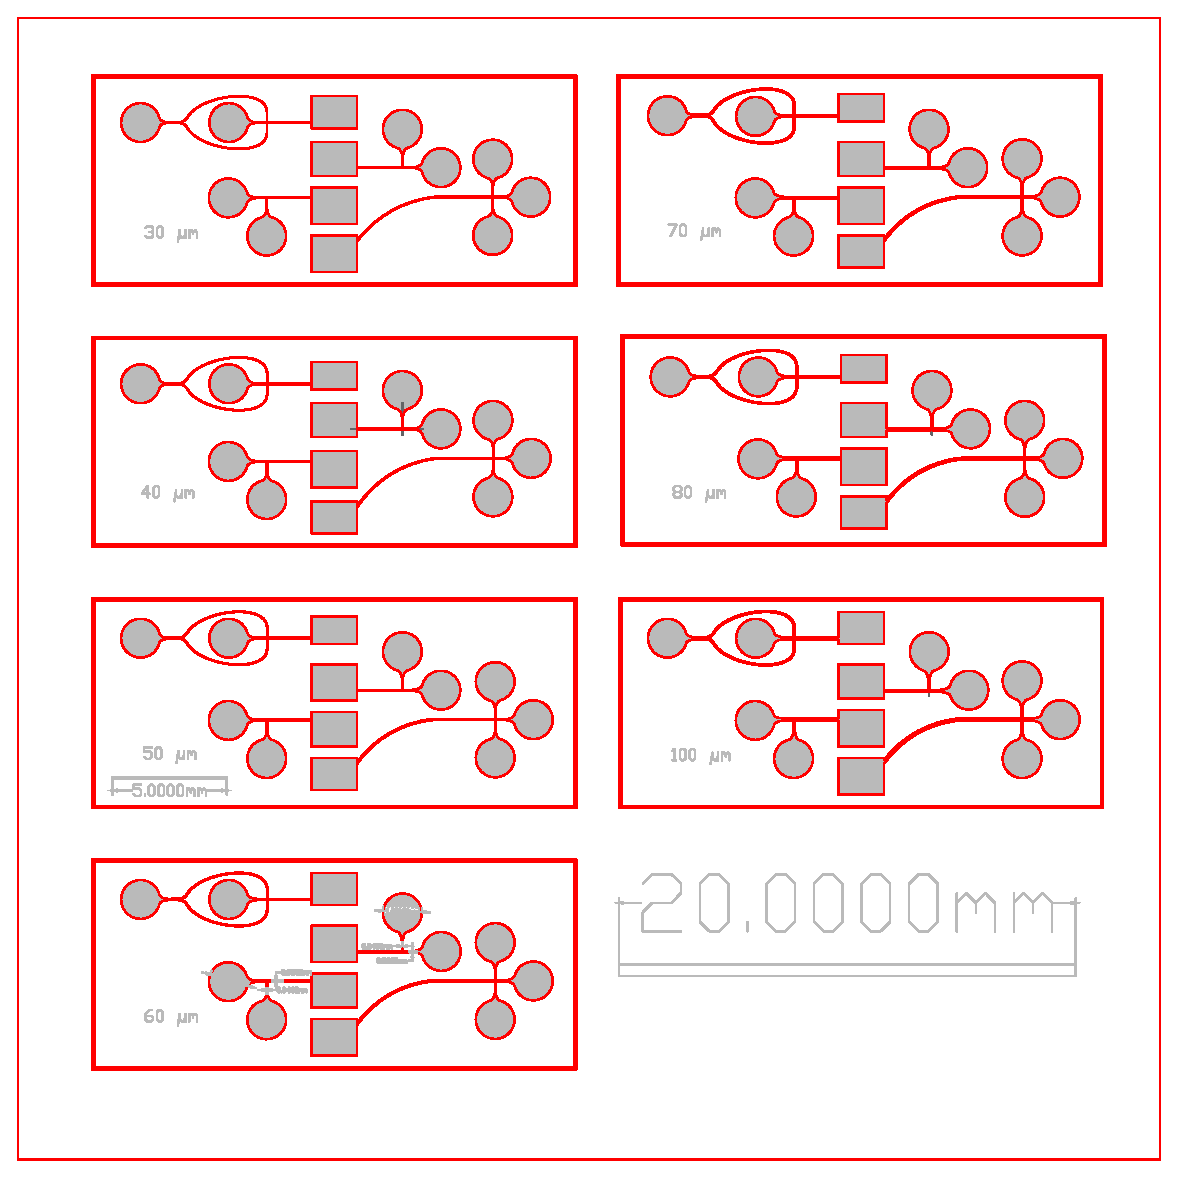
\includegraphics[clip,trim={0mm 0mm 0mm 0mm},scale=.4]{Ressourcen/IMG/Microfluidics_Prototype_3_2018412-Layout_eval_compl}
		\caption{Layout of one rectangular mask for a \SI{3}{\inch} - wafer}
		\label{fig:CAD:mask:single}
	\end{subfigure}
	
	\vfill
	\begin{subfigure}[c]{\textwidth}
		\centering
		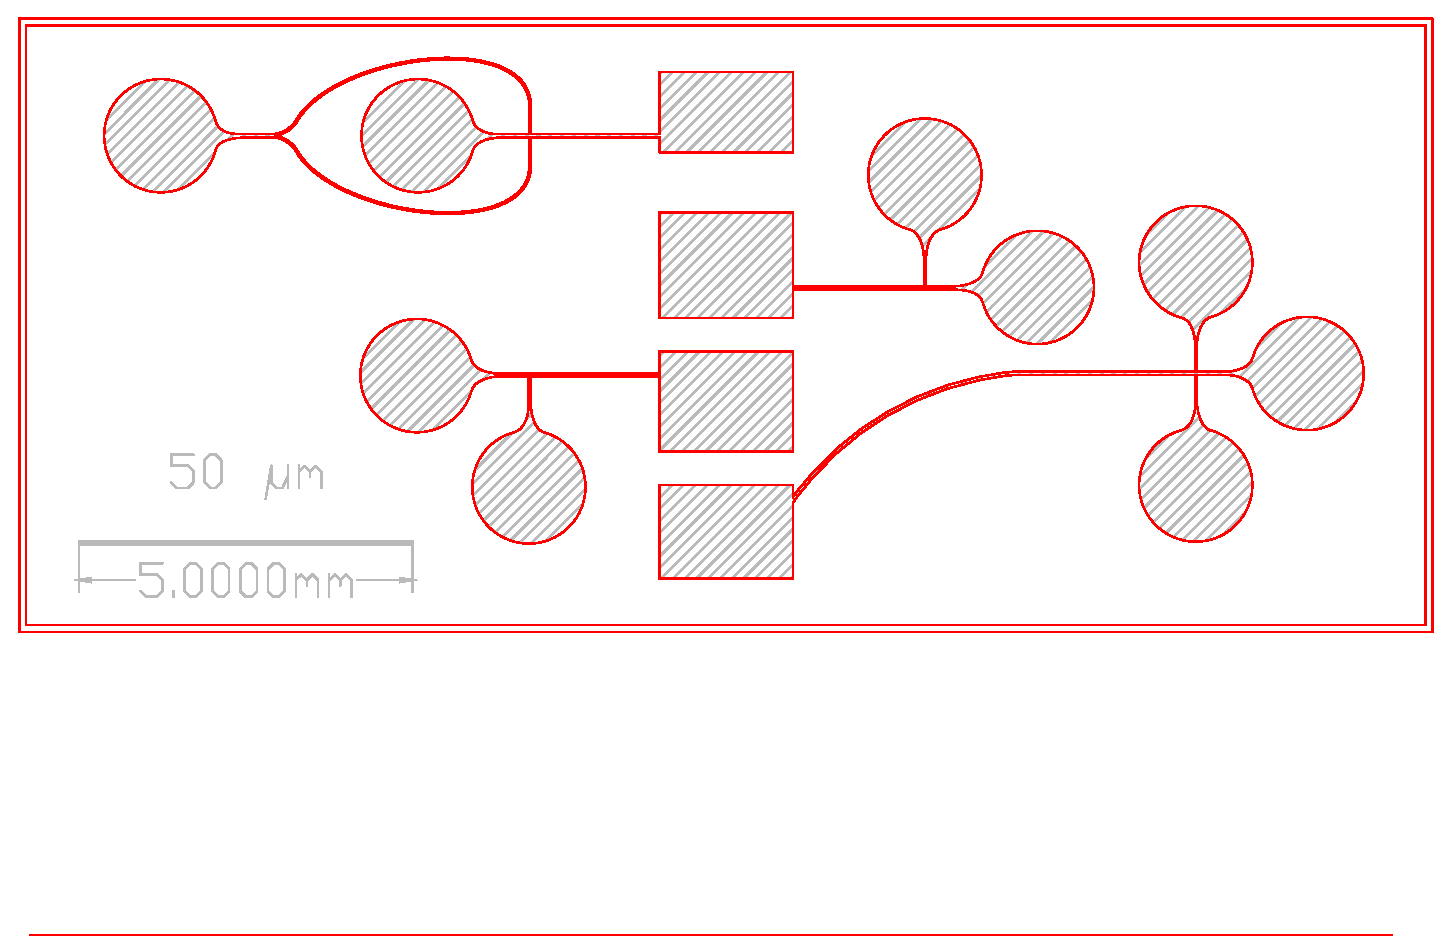
\includegraphics[clip,trim={0mm 50mm 0mm 0mm},scale=.55]{Ressourcen/IMG/Microfluidics_Prototype_3_2018412-Layout_Eval_50um}
		\caption{Layout of a single microfluidic channel-test device, where every main channel is \SI{50}{\micro\meter} wide.}
		\label{fig:CAD:mask:test}
	\end{subfigure}
	
	
	\caption{Three different magnifications of the resulting mask layout. Figure (\protect\subref{fig:CAD:mask:A4}) shows the complete DIN A4 page with the 4x5 array of foil masks. A single mask at position (3,1) is enlarged at (\protect\subref{fig:CAD:mask:single}), where seven fluidic devices in different dimensions from \SIrange{30}{100}{\micro\meter} for tests of the junction layout can be used later. Zoomed into one test layout (\protect\subref{fig:CAD:mask:test}) with a main channel width of \SI{50}{\micro\meter}, there are four previously discussed junction geometries aligned to their reservoirs in the center.} 	
\end{figure}
\clearpage
\newpage


\subsection{Soft Lithography}
\begin{wrapfigure}[17]{r}{0.47\textwidth}
	\includegraphics[scale=.65,trim={0mm 0mm 0mm 8mm}]{Ressourcen/IMG/photolithographic-process-of-microfluidic-mold}%
	\caption{Schematic workflow of soft lithography: Photoresist is spun onto the silicon substrate (1) and exposed by UV-light through a mask (2), which then leads to a patterned resist (3). The master mold is acquired after development to remove the residual, soluble resist (4).  \cite{lit:nano:eveflow}}
	\label{fig:lithography:mold}
\end{wrapfigure}
To print the designed masks negatively on the \SI{3}{\inch} - Si-substrate (\SI{600}{\micro\meter}, Silicon Materials e.K.), standard Soft-Lithography has been used. Due to the fact, that a channel's height depends on the film thickness, which in turn correlates to the spinning parameters and the composition of the resist, the desired channel height of about \SIrange{25}{30}{\micro\meter} could be reached with epoxy resin (SU-8 3025, MicroChem Corp.) and a spin speed of \SI{3000}{\per\minute}.\\
For larger test structures (as in Figure \ref{fig:CAD:mask:single}) I also produced chips with a height of approx. \SI{50}{\micro\meter} with SU-8 3050 (MicroChem Corp.) at \SI{3000}{\per\minute}. Before, the wafers were heated over \SI{120}{\degreeCelsius} for \SI{60}{\minute} in a drying oven to brake up the hydrogen bonds and ensure proper resist adhesion to the substrate.

After the spin process, the silicon wafer was soft-baked on a hot-plate for \SI{5}{\minute} at \SI{65}{\degreeCelsius} and \SI{60}{\minute} at \SI{95}{\degreeCelsius} and subsequently cooled to room temperature with \SI{5}{\degreeCelsius\per\minute}. Then, the desired foil mask was mounted into a manual mask-aligner (MJB3, SÜSS MICROTEC SE).
This mask was brought in contact to the surface of photoresist and the UV light, generated by a \SI{200}{\watt} Hg-source, was guided through it on exposed resist parts for \SI{54}{\second}.\\
On these spots, the cross-linked resist built short resin-chains, which polymerized during the Post Exposure Bake of \SI{5}{\minute} at \SI{65}{\degreeCelsius} and \SI{5}{\minute} at \SI{95}{\degreeCelsius}. As last step, the substrate was immersion washed in MicroChem's SU-8 developer for 10-\SI{12}{\minute}, rinsed with \acrfull{abbr:ipa} afterwards to remove the acid developer resp. residual resist and dried with N$_2$.
\newpage
With these negative mold, microchannels in PDMS (Sylgard 184, DOWSIL) could be produced. Foremost, PDMS was well mixed in a ratio of 10:1 with curing agent and poured over the master mold in a plastic petri dish. To get rid of the solvent, the dishes were put carefully inside a desiccator under a vacuum of \SI{200}{\hecto\pascal} until all bubbles were removed. \\
Complete curing of the PDMS proceeded by baking at \SI{60}{\degreeCelsius} for at least an hour (Figure \ref{fig:lithograyphy:pdms}.1 and .2). Eventually, the dish was carefully destroyed because of the fragile silicon wafer and the PDMS could be peeled off its master mold (Figure \ref{fig:lithograyphy:pdms}.3). The round siloxane piece was then cut with razor blades or scalpels inward the narrow border lines. Inlets from the top were pierced all the way through into the silicone using sharpened dispensing tips (\SIrange{0.51}{0.71}{\mm}, Nordson EFD) and biopsy punchers (\SI{0.5}{\mm}, World Precision Instrument, Fisher Scientific) (Figure \ref{fig:lithograyphy:pdms}.4).

\begin{figure}[tb!]
	\begin{subfigure}[t]{0.49\linewidth}
		\centering
		\includegraphics[height=0.15\textheight]{Ressourcen/IMG/mold1}
	\end{subfigure}
	\hfill
	\begin{subfigure}[t]{0.49\linewidth}
		\centering
		\includegraphics[height=0.16\textheight]{Ressourcen/IMG/mold2}
	\end{subfigure}
	\caption{Workflow of microchannel fabrication: Mixed PDMS with curing agent is poured on the master mold (1,2). Both parts are separated after drying (3) and in- and outlets get punched into the device (4). Plasma treatment (5) -  substitutionary for one bonding strategy - is applied to the PDMS and its counterpart, which are then aligned on each other for permanent adhesion.}
			\label{fig:lithograyphy:pdms}
\end{figure}

\subsection{PDMS Bonding Techniques}
For PDMS bonding to SiN, PDMS or glass surfaces uncured PDMS was used as an adhesive layer. PDMS was spun onto a cleaned Si-wafer at \SIrange{6000}{9999}{\per\minute} for at least \SI{5}{\minute} as glue. The microchannel was dipped slightly onto the silicon in order to let the liquid not get sucked into the channels by capillary forces. It was wiped off another time on a microscope slide to thin out the layer of glue further and then aligned to GMR-structures on the silicon chip inside the PCB under a stereo microscope. To harden the fresh PDMS every chip was put again into the drying oven for \SI{60}{\minute} at \SI{60}{\degreeCelsius}.\cite{lit:fluidics:pdms_bonding}
 \newpage
Another approach, which was used for the very first channels, was joining the PDMS device and a cured, plain PDMS piece  without any adhesive by just cleaning both surfaces with \SI{99}{\percent} acetone and \SI{99}{\percent} IPA. Before bringing both parts in contact, drying them in filtered air or nitrogen has been optional. Devices built in this manner were water-tight, but had a very low pressure resistance. Nevertheless droplet generation in these channels was possible, although not stable over more than \SI{10}{\minute} as the hydraulic resistance in a channel scales with the third power of the rectangular channel's cross section area.\cite{lit:fluidics:BioMEMS}
 
Lastly, I tried to establish oxygen plasma cleaning both surfaces before linking them. Plasma cleaning aims to remove organic as well as hydroxy groups from a substrate by RF activated O$_2$ gas under vacuum. The reaction of free radicals with the particular groups forms products with lower vapor pressure that are evacuated under vacuum and constant O$_2$ influx. Bringing two parts treated suchlike together binds them at generated polar functional groups, which is in this case mainly the silanol group (Si-OH).\\
Before exposing either two pieces of PDMS or one piece PDMS and a glass microscopy slide to the plasma, every part was washed in \SI{99}{\percent} acetone and \SI{99}{\percent} IPA and dried in a oven for 30-\SI{60}{\minute} at \SI{60}{\degreeCelsius}. The environment in the chamber was at first evacuated to \SI{200}{\milli\torr}, then constant oxygen influx of \SI{10}{\sccm} to \SI{600}{\milli\torr} vacuum was set. The pieces were cleaned by \SI{70}{\watt} plasma for 20-\SI{40}{\second} and joined immediately after ventilation of the chamber. Although the process was supposed to show its effect instantaneously, the united channels were baked again for \SI{60}{\minute} at \SI{60}{\degreeCelsius}.\cite{lit:fluidics:plasma_treatment}
\newpage
\section{Numerical Droplet Simulation}
Computation of a droplet with defined dimensions flowing over the GMR half-bridge and an evaluation of the resulting magnetic field as well as the output signal was determined to be the first part of this work. After establishing MATLAB functions for numerically calculating the particle distribution inside the droplet and trying different approaches for the signal simulation, the algorithms were implemented into a graphical user interface (\acrshort{abbr:gui}) for an effortless workflow as seen in figure \ref{fig:sim:GUI}. The goal of this work was to show whether a signal with enough amplitude could be measured at a defined particle concentration. Afterwards, an extension for generating a spherical singularity with particles on the surface, as a model for a cell inside a droplet, was also implemented.
\subsection{Shape Evaluation}
\label{sec:sim:shape_eval}
The first question to be asked was: How can the water droplet in the continuous oil phase be modeled without using the complexity of a lattice Boltzmann Method or equally precise numerical models as described in the literature?\cite{lit:fluidics:droplet:simulation:t}\cite{lit:fluidics:droplet:junction:cross} Therefore, two models derived from basic assumptions, were created and tested in MATLAB.
The first assumption focused on the influence of channel walls on the sides of a droplet. In plug droplets (where the length is larger than width and height) should form a cuboid shaped center. Secondly, I assumed that the interfacial tension between the two phases would cause a cylindrical tip similar to a Poiseuille-flow profile (Figure \ref{fig:sim:cubcyl}). In contrast, a spherical tip approach as described in this paper's model should be also evaluated (Figure \ref{fig:sim:cubsph}, \ref{fig:sim:cylsph}).\cite{lit:fluidics:droplet:junction:cross}
\newpage
In the MATLAB model, different shapes were achieved using the correct boundary conditions to a defined center of one droplet.
That means, the boundary conditions for the cuboid center were on the one hand side in height and width the (user specified) channel dimensions and on the other side the difference of the complete length of a droplet and a half of the major room dimension. In particular, the maximum of the plug's width and height equals the later radius of the spherical tip, whereas the width equals to the radius in the cylindrical model.
\begin{equation}
L_{cub} = L_{Droplet} - \frac{\max \{ H_{Droplet},W_{Droplet}\}}{2}
\label{eq:l_cub}
\end{equation}

Problematic was, that the interface between a sphere and a cuboid (Figure \ref{fig:sim:cubsph}) is not as continuous as in the other cases. That not only led to the rejection of the Cuboid-Sphere-Model, but also to the insight that a projection from the circle to a rectangle or square, which are the bases of both geometric objects, is not solvable without inefficient extra effort.\\
This was afterwards solved by implementing a cylinder instead of a cubic center (Figure \ref{fig:sim:cylsph}) for matching the interfaces (Particle\_Distribution\_Cylinder\_Sphere.m), but also rejected due to the lacking precision in a major part of the plug.
Hence, the droplet simulation was constructed to generate a cuboid shaped center with two cylindrical halves on the corresponding tips (Figure \ref{fig:sim:cubcyl}). (Particle\_Distribution\_Cylinder\_Cuboid.m)
\begin{figure}
	\begin{subfigure}[t]{0.32\textwidth} 
		\centering
		\includegraphics[width=\linewidth]{Ressourcen/IMG/CubCyl}
		\caption{Cylinder Cuboid}
		\label{fig:sim:cubcyl}
	\end{subfigure}
	~
	\begin{subfigure}[t]{0.32\textwidth} 
		\centering
		\includegraphics[width=\linewidth]{Ressourcen/IMG/CubSph}
		\caption{Sphere Cuboid}
		\label{fig:sim:cubsph}
	\end{subfigure}
	~
	\begin{subfigure}[t]{0.32\textwidth} 
		\centering
		\includegraphics[width=\linewidth]{Ressourcen/IMG/CylSph}
		\caption{Sphere Cylinder}
		\label{fig:sim:cylsph}
	\end{subfigure}
	
	\caption{Shape evaluation at different droplets, sub-figure (\protect\subref{fig:sim:cubsph}) shows the problem of mapping a circular shape on a round shape.} 
	
\end{figure}
\newpage
\subsection{Particle Distribution and Configuration inside a Droplet}
For the magnetic field in the plug, there had to be particles distributed inside the boundaries. The most important factor for the later evaluation was the concentration of the nano-spheres, because it could be also practically influenced. However, in the MATLAB simulation the basic premise was the constant scalar magnetic field of one particle as a dot in space.
\subsection{Equal Particle Distribution inside a Droplet}
In the end, these particles should be equally distributed over the whole plug, but in the model over three volumes, the center and both tips. Therefore, after parsing the input and initialization, the complete volume of a plug was computed by using Equation \ref{eq:l_cub} for
\begin{align}
V_{plug} &= V_{cub} + 2 \cdot V_{cyl,half} \\
& = L_{cub} W_{Droplet} H_{Droplet}\ +\ 2 \cdot ( 0.5 \cdot \bigg(\frac{W_{Droplet}}{2}\bigg)^2 H_{Droplet}\ \pi)
\label{eq:volume}
\end{align}
For the amount of particles, the relations between $V_{cub}/V_{plug}$ and $V_{cyl,half}/V_{plug}$ were multiplied with the end concentration and rounded to an integer. 

Then, the script loops for every particle in the cuboid to create three spatial coordinates with the $rand()$ C-function for random distribution with the boundary conditions from \ref{sec:sim:shape_eval}. In programming to generate a randomly distributed interval with $rand()$, which gives only numbers between 0 and 1, following correlation can be applied:
\begin{equation}
r = a + (b-a)\ \cdot\ rand(),\ \mathrm{for\ an\ Interval}\ I = [a,b]
\end{equation}
As the origin of the coordinate system was specified to be at $[0,0,0]$, the interval limits had to be in x-Direction $[-L_{cub}/2,\ L_{cub}/2]$, in y-Direction $[-W_{Droplet}/2,\ W_{Droplet}/2]$ and in z-Direction $[-H_{Droplet}/2,\ H_{Droplet}/2]$.

After the arrangement of particles in the center, the program loops for the amount in the tips. For the first time, creation of points inside the cylindrical tips was done by an equal distribution of three cylinder coordinates $r \in [0,W_{Droplet}/2],\ \theta \in [0,2\pi)$ and $h \in [-H_{Droplet}/2,H_{Droplet}/2] $ and then by back-transformation to the Cartesian coordinates via eq. \ref{eq:distr:wrong}. That was realized to be wrong, as the area element of a circle is given by eq. \ref{eq:distr:surf_element}, which then gives a higher concentration of points near the center than the outside (Figure \ref{sim:distr:wrong}, left).\cite{lit:sim:sphere_point_picking}
\begin{align}
x & = r\ sin \theta,\ y = r\ cos \theta,\ z = h \label{eq:distr:wrong}\\
dA &= 2\pi r\ dr \label{eq:distr:surf_element}\\
x & = \sqrt{r}\ sin \theta,\ y = \sqrt{r}\ cos \theta,\ z = h \label{eq:distr:corr}
\end{align}

\begin{wrapfigure}[9]{r}{0.53\linewidth}
	\centering
	\includegraphics[scale=.4]{Ressourcen/IMG/CircularDistributionError}
	\caption{Particle Distributions inside a circle with randomly initialized parameters, left side with Eq. \ref{eq:distr:wrong}, right side with Eq.  \ref{eq:distr:corr} \cite{lit:sim:disk_point_picking}}
	\label{sim:distr:wrong}
\end{wrapfigure}
The correct point picking for a half cylinder resulted in equations \ref{eq:distr:corr}. The angular cylinder variables $\theta_1$ and $\theta_2$ for front and rear tips thus had to be initialized inside $I_1 = [0,\pi]$ and $I_2 = [\pi,2\pi]$.\cite{lit:sim:disk_point_picking} Of course, these halves had to be moved outside the origin to the relative end of the cuboid by subsequently adding to the x-coordinate either $\pm\ L_{cub}/2$. Moreover, the user is also able to shift the particle for the later simulation around the y- and z-direction. There were specified two parameters $off_y$ and $off_z$, which are added to their respective particle coordinates, in order to move the plug in these axes.

\subsubsection{Singularity with Equal Particle Distribution inside the Droplet}
In my model, the cells were ideally presumed as spheroid singularity without nanoparticles inside, but on the surface. The user was, additionally to the upper model, prompted to specify the radius of the singularity $R_{sph,inside}$ in \SIUnitSymbolMicro m, a 3-dim vector with the x-,y- and z-center-position of the singularity inside $Pos_{sph,inside}$ also in \SIUnitSymbolMicro m and the percentage  of particle covered surface of the sphere relatively to the overall surface \\ $Perc_{part\ on\ sph\ surf}$ ($\in [0,1]$).
Following the user input, the script would parse the mentioned, convert the values and set up the droplet dimensions as in the upper case. Then, a relation between the surface areas $A_{sphere}$ and $A_{particle}$ was computed, multiplied by the cover percentage and rounded to the next higher integer for the total amount of $particlesOnSphSurf$.

The next section is a security measure to prevent the user from specifying a sphere-position, which lets the sphere protrude outside the drop. To meet the first condition, the position plus the radius had to lie inside every of the spatial dimensions. Due to the numerical errors of MATLAB at very small numbers, some expressions were considered false by mistake. As countermeasure every side of an expression was multiplied by $10^{10}$. 
On top, a trigonometrical condition for the sphere inside cylindrical tips had also to be met:
\begin{equation}
\sqrt{\big(\lvert Pos_{sph,inside}(1)\rvert - (L_{cub}/2)\big)^2 + Pos_{sph,inside}(2)^2} + r_{sphere}  <= W_{Droplet}/2
\end{equation}
otherwise specific error messages would be generated and the program aborted.\\
According to the sphere's volume, a new concentration for the particles inside the plug had to be computed by the dilution law $c_1v_1 = c_2v_2$, where $c_1$ is the concentration of particles in the droplet without singularity, $c_2$ the concentration with singularity. $v_1$ and $v_2$ thereby are the volumina without and with the cell inside. This equation then is reconstructed to 
\begin{equation}
c_2 = Concentration \cdot \frac{V_{plug}}{V_{plug} - V_{sphere}}
\end{equation}
The resulting amount is used to calculate the number of particles in every tip and the cuboid center. With these values, the distribution loop could start in two different styles: Discarding every point inside and on the surface of the singularity or discarding every point inside and computing the amount of particles on the surface.\bigskip\\
\textbf{Plain, non-magnetic Singularity}
\\
On the one hand side, if the user specified that no particles should be on the surface of the sphere - a model for a non-magnetic cell - the loop would discard every particle inside and on the sphere's surface, which did not fulfill an adapted coordinate equation for a sphere: 
\begin{multline}
\sqrt{(Pos_{sph,inside}(1) - x)^2 + (Pos_{sph,inside}(2) - y)^2 +
	(Pos_{sph,inside}(3) - z)^2} \\<= r_{sphere}
\end{multline}
, where x is the x-coordinate of a particle, y and z analogically.
\newpage
\textbf{Singularity with \glspl{abbr:MNP} on its Surface}
\\
On the other hand side, for a surface-coverage < 1, the algorithm would loop over the total number of points on the sphere. As mentioned above, to get rid of the "Pole-Aggregation" - problem for an equal distribution of the spherical coordinates, the azimuth $\theta$ and zenith $\phi$ were not distributed in $[0,\pi]$ resp. $[0,2\pi]$, but $\theta \in [0,2\pi]$.\\ As the core of that approach, $\phi$ was not distributed equally, merely by equation \ref{eq:sph:points}, which results in a weighted distribution between 0 and $\pi$.
\begin{align}
\phi & = \arccos(2\nu - 1), \nu\in[0,1] \label{eq:sph:points}\\
x &= r\cos(\theta)\sin(\phi) \label{eq:transf:x}\\
y &= r\cos(\phi)\sin(\theta) \label{eq:transf:y}\\
z &= r\cos(\phi) \label{eq:transf:z}
\end{align}
After the statistical part, the spherical components were reverse transformed using \ref{eq:transf:x} - \ref{eq:transf:z} and plotted, if the user set the corresponding flag.\cite{lit:sim:sphere_point_picking}
\subsubsection{Data Storage}
For storing the particle and simulation data, one overall function "SaveWithNumber.m" was established. When the flag 'Simulation' was false, the function would check for an existing folder in the current directory and, if there, also for existing .txt - files with the same parameters. According to how often the same file name was there, the function would then append a running index to the file name. Afterwards the script writes in three comma separated columns the corresponding Cartesian coordinates. If an existing MATLAB figure handle is passed to the Save-Function, this would be also saved into a separate figure folder in the current directory. At successful finish, the script returns the complete absolute path to the newly created data file. 
\clearpage
\newpage
\subsection{\acrfull{abbr:gui}}
As a graphical representation of these functions, a  MATLAB app has been also built with the in-house App Designer. In a modular approach, the user would be prompted at startup in the main window \ref{fig:sim:GUI:main} to select the function for the generation of particles inside a droplet or the simulation over GMR structures. Additionally, this UIFigure shows a stores path to the lastly generated particle data file, which also can be immediately simulated.


At selection of the generation-button, a second window opens in front and displays the parameter values as in \ref{fig:sim:GUI:generation}. Clicking then the start-button starts the distribution function or, if the user selected one kind of singularity inside the droplet, is prompted by another dialog (Graphic \ref{fig:sim:GUI:inner}) to specify further properties. These slider controls adjust their limit dynamically according to the previously defined droplet dimensions. At finish of the function, the droplet is then plotted in side- and top-view at the generation figure.

To simulate the generated data as described in \ref{sec:sim:GMRsim}, the user inputs again his desired values and selects a dataset (Figure \ref{fig:sim:GUI:simulation}). While simulating, a waiting bar is displayed to prevent the user from further unwanted input. At success the droplet signal is plotted in both directions of the sensor plane (x-y-plane). 

\begin{landscape}
	\centering
	\begin{figure}
		\begin{subfigure}{0.49\linewidth} 
			\centering
			\includegraphics[clip,trim={0.5mm 1mm 1mm 2mm}, scale=.7 ]{Ressourcen/IMG/GUI_main}
			\caption{Main window of the GUI with the choice of particle data generation or droplet-over-GMR simulation. The last generated particle file is processed below an is passed as standard value to the simulation function.}
			\label{fig:sim:GUI:main}
		\end{subfigure}
		\hfil
		\begin{subfigure}{0.49\linewidth} 
			\centering
			\includegraphics[clip,trim={1mm 1mm 1mm 2mm},scale=.4]{Ressourcen/IMG/GUI_generation}
			\caption{Generation window, where the user can actuate droplet dimensions, offsets, particle concentration and content with or without singularity. Additionally, he can output an external live-plot figure and different shapes, which are under construction.}
			\label{fig:sim:GUI:generation}
		\end{subfigure}
		\vfil
		\begin{subfigure}{0.49\linewidth} 
			\centering
			\includegraphics[clip,trim={0.5mm 0 0 2mm},scale=.33]{Ressourcen/IMG/GUI_inner}
			\caption{Further specifications of the sphere inside the droplet are possible in this figure. The ranges of the sliders adjust dynamically to every change in order to prevent a shift of the sphere outside the droplet boundaries.}
			\label{fig:sim:GUI:inner}
		\end{subfigure}
		\hfil
		\begin{subfigure}{0.49\linewidth} 
			\centering
			\includegraphics[clip,trim={1mm 1mm 1mm 2mm},scale=.375]{Ressourcen/IMG/GUI_simulation_2}
			\caption{The simulation window lets the user again select an external live-plot and asks for the scale of the signal (Differential Voltage before amplification or magnetic field of the dipole). Selection of the input file and customizing the simulation performance has to be done before starting.}
			\label{fig:sim:GUI:simulation}
		\end{subfigure}
		
		\caption{Different stages of a droplet simulation cycle. At startup the main window (\protect{\subref{fig:sim:GUI:main}}) is displayed, the user specifies the particle distribution in figures (\protect{\subref{fig:sim:GUI:generation}}) and (\protect{\subref{fig:sim:GUI:inner}}) and lastly simulates at specific parameters (\protect{\subref{fig:sim:GUI:simulation}}).} 
		\label{fig:sim:GUI}
		
	\end{figure}
\end{landscape}

\subsection{Algorithms for Simulation of GMR Sensor Signal to Magnetic Droplet Configurations}
\label{sec:sim:GMRsim}
Second part of the MATLAB simulation was to evaluate the signal, which is generated by one particle filled droplet guided over the GMR-sensor. The user had to pass the parameters in Table \ref{tab:sim:params} to the simulation/evaluation script "Simulate\_Droplet\_Measurement.m", whereas the unit and datafile arguments were not essential.
\begin{table}[htb!]
	\begin{tabularx}{\linewidth}{|l|c|C|}
		\hline
		\textbf{Parameter}&\textbf{Unit}&\textbf{Purpose}\\	
		\hline
		filename & [string] & Input file with particle coordinates\\
		\hline
		iteration\_steps & [1] & Amount of simulation loops for precision\\
		\hline
		shift\_from\_origin & [\si{\micro \meter}]& Shift droplet from origin in x-Direction\\
		\hline
		shift\_between\_GMR & [\si{\micro \meter}] & Shift between the two sensors of a double bridge\\
		\hline
		plot\_enabled & [true(1)/ false(0)]& Live plot of simulation\\
		\hline
		unit & 'T' / 'V' & Output signal in units of the magnetic field or the measurement voltage\\
		\hline
		U\_in & [mV] & Amplitude of excitation signal \\
		\hline
		datafile & [string] & Absolute path for a special file to save in\\
		\hline
		
	\end{tabularx}	
	\caption{Function parameters of the simulation script in ascending order}
	\label{tab:sim:params}
\end{table}

At first, the program checks the input, parses the droplet dimensions from the file name and initializes the constants and variables. The needed constants are the vacuum permeability $\mu_0$ ($\SI{4\pi E-7}{\henry\per\meter}$), the length $L_{GMR}$ (\SI{30}{\micro\meter}) and width  $W_{GMR}$ (\SI{2}{\micro\meter}) of one GMR sensor and the magnetic momentum of one particle. This momentum was computed by another external script from the iron concentration and saturation magnetization per kg iron given by the data sheet.\cite{lit:sim:datasheet:50nm}
\begin{equation}
m_{mag,particle} = \frac{M_{sat}\ \Big[\si{\A\meter\squared\per\kilo\gram\Ferrum}\Big]}{\textrm{Particles\ in\ Volume\ of\ 1kgFe}}\bigg[\si{\A\meter\squared\per\particle}\bigg]
\end{equation}
In this work I assumed a magnetic moment of \SI{2.5e-18}{\ampere\meter\squared} for a \SI{50}{\nm} bead, compliant to prior VSM measurements and therefore treated also as constant value.

The distance between a single iteration step is estimated from \[(2\ shift\_from\_origin\ +\ shift\_between\_GMR\ +\ 2W_{GMR})\] divided by the amount of user selected iteration steps. Afterwards, the particle is moved out of the zero-point by relocating it in x-direction by $L_{Droplet}/2\ +\ shift\_from\_origin$ and in z-direction by $H_{Droplet}/2$.
As further simplification and performance enhancement the signal of the second GMR is not determined by the magnetic dipole equation (\ref{eq:mag:dipole:triple_int}), but by an array shift of the first GMR signal. 

\bigskip

The signal response of magnetoresistive sensor due to the presence of magnetic particles suspended in a droplet can be described by a magnetic dipole model. For the generation of this signal were several approaches evaluated: At first - before finding the analytical solution - the numerical integration, then the analytical solution itself and at last another model from Li, Wang and Sun.\cite{lit:sim:wang}

\subsubsection{Numerical Integration}
Initially, I presumed to get the finest results by solving the volume integral of the magnetic field for a magnetic dipole (Eq. \ref{eq:mag:dipole:triple_int}) for every particle in the droplet at every iteration step. This resulted in enormous computational load per single iteration. To simplify further, the GMR sensors were considered to lie in the x-y-plane, which led to a negligible z-component and so reduced the triple to a double integral (Eq. \ref{eq:mag:dipole:double_int}). As that brought only little advantage in performance, different MATLAB integration methods were implemented in order to find the fastest. This could also not reduce the needed processor power significantly, so an analytical solution of the equation had to be found.
\newpage
\subsubsection{Analytical Approach}
The next method to solve for the signal was to evaluate the equation analytically. This was achieved by help of the computing engine Wolfram|Alpha.
For shortenings, the following symbols are introduced:\\
$\chi\ \widehat{=}$ x-coordinate of particle\\
$\phi\ \widehat{=}$ y-coordinate of particle\\
$\psi\ \widehat{=}$ z-coordinate of particle\\
$m_s\ \widehat{=}$ Saturation moment of one particle\\
$z \ \widehat{=}$ Height of the sensor (in my model neglected - hence 0 - but kept for completeness)


The derivation was conducted from the Dipole Momentum Equation substituted with the specified symbols.

\begin{align}
H_{xy} &=  \int\displaylimits_{-\frac{l_{GMR}}{2}}^{\frac{l_{GMR}}{2}} \int\displaylimits_{-\frac{b_{GMR}}{2}}^{\frac{b_{GMR}}{2}} \frac{3\ m_s\big( x- \chi \big) \big(z- \psi\big) }{\sqrt{\big( x- \chi\big)^2 + \big(y- \phi\big)^2 + \big(z- \psi\big)^2}^5}\ dxdy
\label{eq:mag:dipole:double_int}\\
&=3\ m_s\big(z- \psi\big)  \int\displaylimits_{-\frac{l_{GMR}}{2}}^{\frac{l_{GMR}}{2}} \int\displaylimits_{-\frac{b_{GMR}}{2}}^{\frac{b_{GMR}}{2}} \frac{\big( x- \chi \big) }{\sqrt{\big( x- \chi\big)^2 + \big(y- \phi\big)^2 + \big(z- \psi\big)^2}^5}\ dxdy
\end{align}
For clarity, the definite integrals are considered as indefinite for these calculations. It is good practice in mathematics to remove the numerator and afterward the denominator of a non-trivial integral, so the first substitution was determined to be $u = (x-\chi)$, $du = dx$
\begin{equation}
H_{xy} =3\ m_s\big(z- \psi\big)  \int \int\frac{u}{\sqrt{u^2 + \big(y- \phi\big)^2 + \big(z- \psi\big)^2}^5}\ dudy
\end{equation}
To get rid of the multiple variables in the denominator, the  second substitution was chosen to be $v = u^2 + \big(y- \phi\big)^2 + \big(z- \psi\big)^2$, $dv = 2udu$
\begin{equation}
H_{xy} =3\ m_s\big(z- \psi\big)  \int \int\frac{\cancel{u}}{v^{5/2}}\ \frac{dvdy}{2\cancel{u}}
\end{equation}
\newpage
Because of these two substitutions, the inner integral solved after the reverse substitutions to equation \ref{eq:mag:dipole:inner_int}. As the focus lay on the whole and no specific solution, the integration constant $c_1$ could be neglected.
\begin{align}
H_{xy} &=\int\frac{3}{2}\ m_s\big(z- \psi\big)\big( -\frac{2}{3v^{3/2}}\big) + \frac{3}{2}\ m_s\big(z- \psi\big)c_1\ dy\\
&=  \int \frac{\ m_s\big(\psi-z\big) }{\sqrt{u^2 + \big(y- \phi\big)^2 + \big(z- \psi\big)^2}^3} + \frac{3}{2}\ m_s\big(z- \psi\big)c_1\ dy\\
&=  \int \frac{\ m_s\big(\psi-z\big) }{\sqrt{\big( x- \chi\big)^2 + \big(y- \phi\big)^2 + \big(z- \psi\big)^2}^3} + \frac{3}{2}\ m_s\big(z- \psi\big)c_1\ dy \label{eq:mag:dipole:inner_int}\\
&=\ m_s\big(\psi - z\big)  \int \frac{1}{\sqrt{\big( x- \chi\big)^2 + \big(y- \phi\big)^2 + \big(z- \psi\big)^2}^3}\ dy
\end{align}

The same method was applied to the outer integral. A third substitution was determined to get rid of one term under the square root: $w=y-\phi$, $dw=dy$.

\begin{equation}
H_{xy} =\ m_s\big(\psi - z\big)  \int \frac{1}{\sqrt{\big( x- \chi\big)^2 + w^2 + \big(z- \psi\big)^2}^3} dw
\end{equation}

In the last substitution step, the root the denominator should be removed in  except for a term trivial to integrate. The equations \ref{eq:mag:dipole:4.subs_s} and \ref{eq:mag:dipole:4.subs_ds} were chosen as desired.

\begin{align}
s &= \frac{w}{\sqrt{\big( x- \chi\big)^2 + \big(z- \psi\big)^2}
	\label{eq:mag:dipole:4.subs_s}}\\
ds &= \frac{1}{\sqrt{\big( x- \chi\big)^2 + \big(z- \psi\big)^2}}dw
\label{eq:mag:dipole:4.subs_ds}\\
H_{xy} &=\ m_s\big(\psi - z\big) \frac{1}{\sqrt{\big( x- \chi\big)^2 + \big(z- \psi\big)^2}} \int \frac{1}{(s^2+1)^{3/2}}\ ds
\end{align}
\newpage
In this respect, the computed equations solved to eq. \ref{eq:mag:dipole:rev_subs_2} after integration and reverse substitution.
\begin{align}
H_{xy} &=\ \frac{m_s\big(\psi - z\big)}{\big( x- \chi\big)^2 + \big(z- \psi\big)^2} \Bigg( \frac{s}{\sqrt{s^2+1}} + c_2\Bigg)\\
&=\ \frac{m_s\big(\psi - z\big)}{\big( x- \chi\big)^2 + \big(z- \psi\big)^2} \Bigg( \frac{w}{\sqrt{\big( x- \chi\big)^2 + w^2 + \big(z- \psi\big)^2}} + c_2\Bigg) \label{eq:mag:dipole:rev_subs_2}
\end{align}
As mentioned before, the integration constant again reduces to zero, so after another reverse substitution (Eq. \ref{eq:mag:dipole:rev_subs_2}) the analytical solution is equation \ref{eq:mag:dipole:solution}

\begin{equation}
H_{xy}= \frac{\ m_s\big(\psi - z\big)\big(y - \phi\big)}{\sqrt{\big( x- \chi\big)^2 + \big(y- \phi\big)^2 + \big(z- \psi\big)^2}\Big(\big( x- \chi\big)^2 + \big(z- \psi\big)^2\Big)} \label{eq:mag:dipole:solution}
\end{equation}


%Indefinite Integral
%
%\begin{multline}
%H_{xy} =  c_1x\ +\ c_2\ - \\ \frac{m_s\big(y - \phi\big)\big(\psi - z\big)}{\Big(\chi^2 + x^2 - 2\chi x + z^2 - 2 z \psi + \psi^2 \Big)\sqrt{\phi^2 + \chi^2 + x^2 - 2\chi x + y^2 - 2\phi y + z^2 - 2 z \psi + \psi^2}}
%\end{multline}
%
%
%
%Applying binom eq for simplification
%
%\begin{equation}
%H_{xy} =  c_1x\ +\ c_2\ -\ \frac{m_s\big(y - \phi\big)\big(\psi - z\big)}{\Big(\big(\chi-x\big)^2 +\big(\psi-z\big)^2\Big)\sqrt{ \big(\chi-x\big)^2 + \big(\phi-y\big)^2 + \big(\psi-z\big)^2}}
%\end{equation}


The next step then was the evaluation of the method inside the boundaries from the beginning. As the evaluation of an integral with known anti-derivative gives
$\int\limits_{a}^{b}\int\limits_{c}^{d}f(x,y)dxdy = \mathcal{F}(x,y)\big|_{d,b} - \mathcal{F}(x,y)\big|_{c,b} - \mathcal{F}(x,y)\big|_{d,a} + \mathcal{F}(x,y)\big|_{c,a}$, the magnetic field was subsequently found as:



%$\chi\ \widehat{=}$ x-coordinate of particle\\
%$\phi\ \widehat{=}$ y-coordinate of particle\\
%$\psi\ \widehat{=}$ z-coordinate of particle\\
%$m_s\ \widehat{=}$ Saturation moment of one particle

\begin{align}
H_{xy} = & \frac{m_s\Big(\frac{l_{GMR}}{2} - \phi\Big)\Big(\psi - z\Big)}{\bigg(\Big(\chi-\frac{b_{GMR}}{2}\Big)^2 +\Big(\psi-z\Big)^2\bigg)\sqrt{ \Big(\chi-\frac{b_{GMR}}{2}\Big)^2 + \Big(\phi-\frac{l_{GMR}}{2}\Big)^2 + \Big(\psi-z\Big)^2}}
\nonumber\\
&-\frac{m_s\Big(-\frac{l_{GMR}}{2} - \phi\Big)\Big(\psi - z\Big)}{\bigg(\Big(\chi+\frac{b_{GMR}}{2}\Big)^2 +\Big(\psi-z\Big)^2\bigg)\sqrt{ \Big(\chi+\frac{b_{GMR}}{2}\Big)^2 + \Big(\phi+\frac{l_{GMR}}{2}\Big)^2 + \Big(\psi-z\Big)^2}}
\nonumber\\
&-\frac{m_s\Big(-\frac{l_{GMR}}{2} - \phi\Big)\Big(\psi - z\Big)}{\bigg(\Big(\chi-\frac{b_{GMR}}{2}\Big)^2 +\Big(\psi-z\Big)^2\bigg)\sqrt{ \Big(\chi-\frac{b_{GMR}}{2}\Big)^2 + \Big(\phi+\frac{l_{GMR}}{2}\Big)^2 + \Big(\psi-z\Big)^2}}
\nonumber\\
&+\frac{m_s\Big(\frac{l_{GMR}}{2} - \phi\Big)\Big(\psi - z\Big)}{\bigg(\Big(\chi+\frac{b_{GMR}}{2}\Big)^2 +\Big(\psi-z\Big)^2\bigg)\sqrt{ \Big(\chi+\frac{b_{GMR}}{2}\Big)^2 + \Big(\phi-\frac{l_{GMR}}{2}\Big)^2 + \Big(\psi-z\Big)^2}}
\end{align}


%MATLAB Code
%\begin{align}
%Out_{x} =\frac{m_s\Big(\frac{l_{GMR}}{2} - particle(2,i)\Big)\Big(particle(3,i) - z\Big)}{\Big(\Big(particle(1,j)-\frac{b_{GMR}}{2}\Big)^2 +\Big(particle(3,i)-z\Big)^2\Big)\sqrt{ \Big(particle(1,j)-\frac{b_{GMR}}{2}\Big)^2 + \Big(particle(2,i)-\frac{l_{GMR}}{2}\Big)^2 + \Big(particle(3,i)-z\Big)^2}}\\
%+\\
%\frac{m_s\Big(-\frac{l_{GMR}}{2} - particle(2,i)\Big)\Big(particle(3,i) - z\Big)}{\bigg(\Big(particle(1,j)+\frac{b_{GMR}}{2}\Big)^2 +\Big(particle(3,i)-z\Big)^2\bigg)\sqrt{ \Big(particle(1,j)+\frac{b_{GMR}}{2}\Big)^2 + \Big(particle(2,i)+\frac{l_{GMR}}{2}\Big)^2 + \Big(particle(3,i)-z\Big)^2}}\\
%-\\
%\frac{m_s\Big(-\frac{l_{GMR}}{2} - particle(2,i)\Big)\Big(particle(3,i) - z\Big)}{\bigg(\Big(particle(1,j)-\frac{b_{GMR}}{2}\Big)^2 +\Big(particle(3,i)-z\Big)^2\bigg)\sqrt{ \Big(particle(1,j)-\frac{b_{GMR}}{2}\Big)^2 + \Big(particle(2,i)+\frac{l_{GMR}}{2}\Big)^2 + \Big(particle(3,i)-z\Big)^2}}\\
%-\\
%\frac{m_s\Big(\frac{l_{GMR}}{2} - particle(2,i)\Big)\Big(particle(3,i) - z\Big)}{\bigg(\Big(particle(1,j)+\frac{b_{GMR}}{2}\Big)^2 +\Big(particle(3,i)-z\Big)^2\bigg)\sqrt{ \Big(particle(1,j)+\frac{b_{GMR}}{2}\Big)^2 + \Big(particle(2,i)-\frac{l_{GMR}}{2}\Big)^2 + \Big(particle(3,i)-z\Big)^2}}
%\end{align}
\subsubsection{Paper Approach for Analytical Solution in x- and y-Direction}
The paper of \citet{lit:sim:wang} proposed a new analytical model for spin valves actuated by \glspl{abbr:MNP} to get a relation of signal per particle. It was implemented as a validation for my computed method and as it had also a magnetic field component in y-direction, which was neglected in the analysis until now. They started their calculations as this model with the Dipole Equation \ref{eq:mag:dipole:triple_int}, where their limits (lxwxh) were chosen as the free layer dimensions of the GMR stack. 
\begin{equation}
\mathbf{H} = \int\displaylimits_{-\frac{l}{2}}^{\frac{l}{2}} \int\displaylimits_{-\frac{w}{2}}^{\frac{w}{2}}\int\displaylimits_{-\frac{h}{2}}^{\frac{h}{2}}\left[{3({ \mathbf{m}}\cdot{\mathbf{r}}){\mathbf{r}}\over r^{5}}-{{\mathbf{m}}\over r^{3}}\right]dxdydz
\label{eq:mag:dipole:triple_int}
\end{equation}

The vector ${\mathbf r}=(x-x_{p})\hat{x}+(y-y_{p})\hat{y}+(z-d)\hat{z}$ was then set up with the unity vectors $\hat{x}$, $\hat{y}$ and $\hat{z}$ scaled by the distances of a particle from the GMR, so the field components resulted to equations \ref{eq:sim:wang:x} and \ref{eq:sim:wang:y}.

\begin{align}
\overline{H}_{x}=&\,{m_{x}\over lw}\left[{x_{r}\over q_{3}^{2}}\left({y_{b}\over r_{2}}-{y_{t}\over r_{3}}\right)+{x_{l}\over q_{1}^{2}}\left({y_{t}\over r_{4}}-{y_{b}\over r_{1}}\right)\right]\nonumber\\
&+{m_{y}\over lw}\left({1\over r_{1}}-{1\over r_{2}}+{1\over r_{3}}-{1\over r_{4}}\right)\nonumber\\
&+{m_{z}\over lw}\left[{d\over q_{3}^{2}}\left({y_{t}\over r_{3}}-{y_{b}\over r_{2}}\right)+{d\over q_{1}^{2}}\left({y_{b}\over r_{1}}-{y_{t}\over r_{4}}\right)\right]
\label{eq:sim:wang:x}
\end{align}

\begin{align}
\overline{H}_{y}=&\,{m_{y}\over lw}\left[{y_{b}\over q_{2}^{2}}\left({x_{r}\over r_{2}}-{x_{l}\over r_{1}}\right)+{y_{t}\over q_{4}^{2}}\left({x_{l}\over r_{4}}-{x_{r}\over r_{3}}\right)\right]\nonumber\\
&+{m_{x}\over lw}\left({1\over r_{1}}-{1\over r_{2}}+{1\over r_{3}}-{1\over r_{4}}\right)\nonumber\\
&+{m_{z}\over lw}\left[{d\over q_{2}^{2}}\left({x_{l}\over r_{1}}-{x_{r}\over r_{2}}\right)+{d\over q_{4}^{2}}\left({x_{r}\over r_{3}}-{x_{l}\over r_{4}}\right)\right]
\label{eq:sim:wang:y}
\end{align}

\newpage
$m_x$,$m_y$ and $m_z$ have been considered as scalar items of the magnetic momentum $\mathbf{m}$, but through the saturation magnetization of the beads in z-direction, the other both could be neglected. Therefore the upper equations both reduced to their last term. The variables were computed after the following dependencies:
$x_{l}=-l/2-x_{p},\ x_{r}=l/2-x_{p},\ y_{b}=-w/2-y_{p},\  y_{t}=w/2-y_{p},\ r_{1}=\sqrt{x_{l}^{2}+y_{b}^{2}+d^{2}},\ r_{2}=\sqrt{x_{r}^{2}+y_{b}^{2}+d^{2}},\ r_{3}=\sqrt{x_{r}^{2}+y_{t}^{2}+d^{2}},\ r_{4}=\sqrt{x_{l}^{2}+y_{t}^{2}+d^{2}},\ q_{1}=\sqrt{x_{l}^{2}+d^{2}},\ q_{2}=\sqrt{y_{b}^{2}+d^{2}},\ q_{3}=\sqrt{x_{r}^{2}+d^{2}},\ q_{4}=\sqrt{y_{t}^{2}+d^{2}}$

The resulting signal was compared to my analytically produced output and showed a overall difference at a simulation precision of 0.01\%. This difference was caused due to the disproportional influence of a singe particle in the ideals simulations, whereas this would be never visible in the noise of a real signal. 
\begin{figure}[h!]
	\centering
	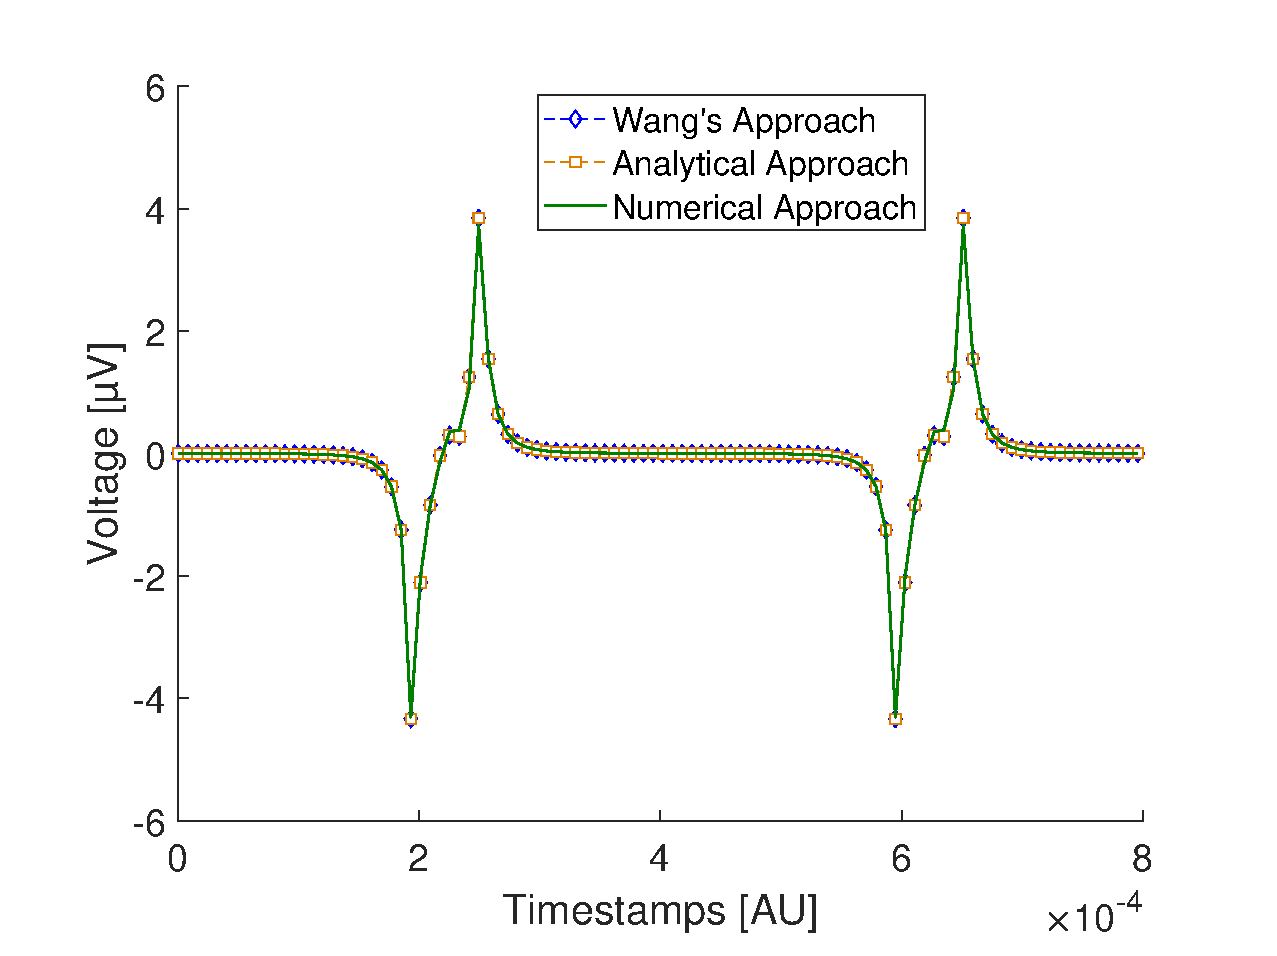
\includegraphics[clip,width=\linewidth]{Ressourcen/IMG/All_three_approaches}
	\caption{An overlay of all three approaches with the numerical simulation in green, the analytical solution in orange squares and Wang et al.'s approaches in blue hashes. A difference between the three signals is not visible, the absolute precision error lies at \num{1E-4}.}
	\label{fig:sim:all_three}
\end{figure}
\newpage

\section{Experimental Analysis of Droplets by Optical and Magnetic Means}
To form plug droplets, I used plain 50 nm MNPs (nanomag-D-spio, Micromod GmbH) at different dilutions (1:0;1:1;1:5)  in Dulbecco’s phosphate buffered saline (PBS, $\eta_{PBS} = \SI{1.05}{\milli\pascal\second}$, VWR) as the dispersed phase and mineral oil (M5904, $\eta_{oil}=\SI{13.8}{\milli\pascal\second}$, Sigma) with 2\%  Sorbitan oleate (Span 80, $\eta_{Span80} =\SI{1000}{\milli\pascal\second} - \SI{2000}{\milli\pascal\second}$,Sigma) as the continuous phase. Span 80 was necessary to facilitate stable generation of drops. For another experiment, I used streptavidin-coated \SI{2}{\micro\meter} Beads (micromer-M, Micromod GmbH). A constant laminar flow was established by a pulsation-free syringe pump system (Nemesys, cetoni GmbH) connected via precision syringes (\SI{250}{\micro\liter}, Hamilton) and PVC tubing (inner diameter \SI{0.5}{\mm}, Reichelt Chemietechnik GmbH) to the microfluidics.
Inside the microchannels, droplets were achieved as well in dripping as in squeezing regime at flow rates of \SIrange{0.3}{3}{\nano\liter\per\second} of the dispersed and \SIrange{0.5}{5}{\nano\liter\per\second} of the continuous phase, without dropping below the flow ratio $\delta > \SI{10}{\percent}$.

\newpage
\subsection{Optical Droplet Tracking}
In order to relate one droplet's velocity and size to a measured electrical signal shape, optical evaluation of droplet formation, size, and velocity was performed. The captured videos under a microscope (DM6 M, Leica Microsystems GmbH) with a sCMOS-camera (DFC9000 GT, Leica Microsystems GmbH) at its minimal frequency were at first separated into their frames in Tagged Image File format. Then, a MATLAB script was adapted to loop over every image and converts it to an greyscale map. In the next step, a Canny Edge Detector algorithm at a threshold value of \SI{70}{\percent} with five steps is applied:\cite{lit:tracking:ellipse_detection}
\begin{enumerate}
	\item Noise-smoothing applying a Gaussian filter
	\item Computation magnitude of the gradient of the filtered image (intensity) and normalizing by its maximum value
	\item Determination of detection hysteresis and its threshold plus Non-Maximum Suppression
	\item Classification of found edges and further filtering
	\item Blob analysis for enhanced hysteresis
\end{enumerate}

Non-Maximum Suppression means the comparison of one pixels edge strength in descending gradient directions and its rejection if a pixel with higher strength is found. This causes a 'edge thinning' of the found lines. After this, in another threshold step edge pixels are classified into "bigger than a high threshold value", "in between thresholds" and "below the low threshold value". The last ones are immediately discarded, while the other two clusters are analyzed in respect to their 8 neighbor pixels. Hence, it can be assumed if the regarded pixel belongs to a strong edge or is noise.\\
The resulting edge picture is then Hough transformed into an accumulator space to apply the feature extraction algorithm for extracting the elliptical shape of a droplet. Because an ellipse can be parametrized with its major and minor axis, one can evaluate the major axis between every pixel pair and then get the minor axis.\cite{lit:tracking:ellipse_detection} As this brute-force method is critically dependent on the complexity of the data set, some restrictions such as ellipse angle, minor/major ax-thresholds as well as Gaussian smoothing have to be brought into consideration to lower memory consumption and enhance the algorithm's performance.


At finish, the six best ellipse fits are returned and plotted. For analysis, the rotation and lengths of the axes are averaged and also plotted. Additionally, at every step the computed values are compared to the previous time step. That gives a rough error estimation and also the velocity by finding Euclidean norm of the ellipse center with its position of the former frame and multiplying it by the frame rate. 
\begin{figure}[h]
	\centering
	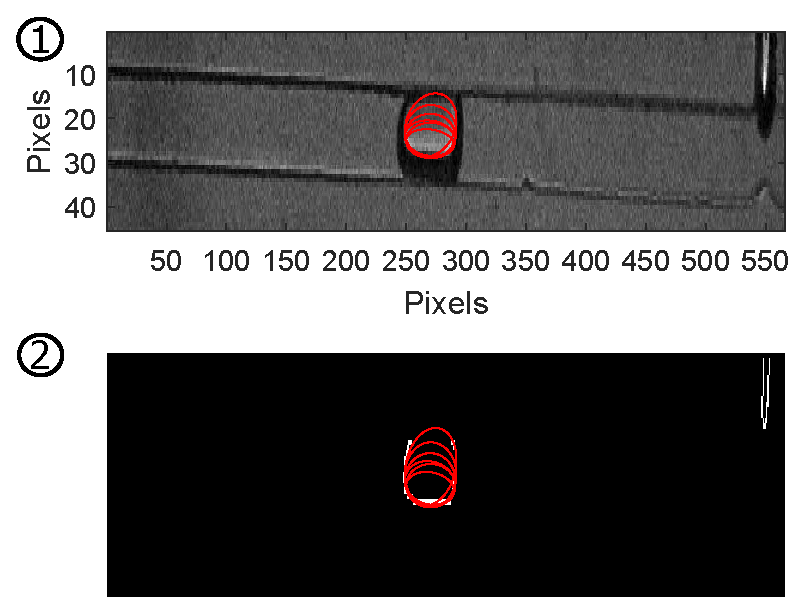
\includegraphics[clip,width=\linewidth,trim={0 0 0 0mm}]{Ressourcen/Tracking/LiveFitting}
	\caption{Picture (1) displays an input image from the microscope in its pixel dimension with the transferred fit from below, picture (2) its processed variant after applying the Canny Edge Extractor with a threshold of \SI{70}{\percent} and fitting the ellipses into it. A high variance in th ellipse minor axes can be observed, while the major axis fits very accurate.}
	\label{fig:tracking:livefitting}
\end{figure}
It also had to be considered to utilize another boundary condition if there was more than one droplet in a frame. Therefore, a center movement threshold condition was used, which limited the possible radius the droplet center's position could change over two frames.\\ In order to enhance the time consumption further, a randomization as in this paper was implemented, which uses a stochastically generated subset of pairs for the examination of the major axes.\cite{lit:tracking:randomization}
\newpage

\subsection{Experimental Data Analysis via MATLAB}
The experimentally gained signal of the Wheatstone half bridge had to be analyzed in regards to peak-height, -distance, -integral and full width at half maximum.
\begin{wrapfigure}[11]{r}{0.55\textwidth}
	\centering
	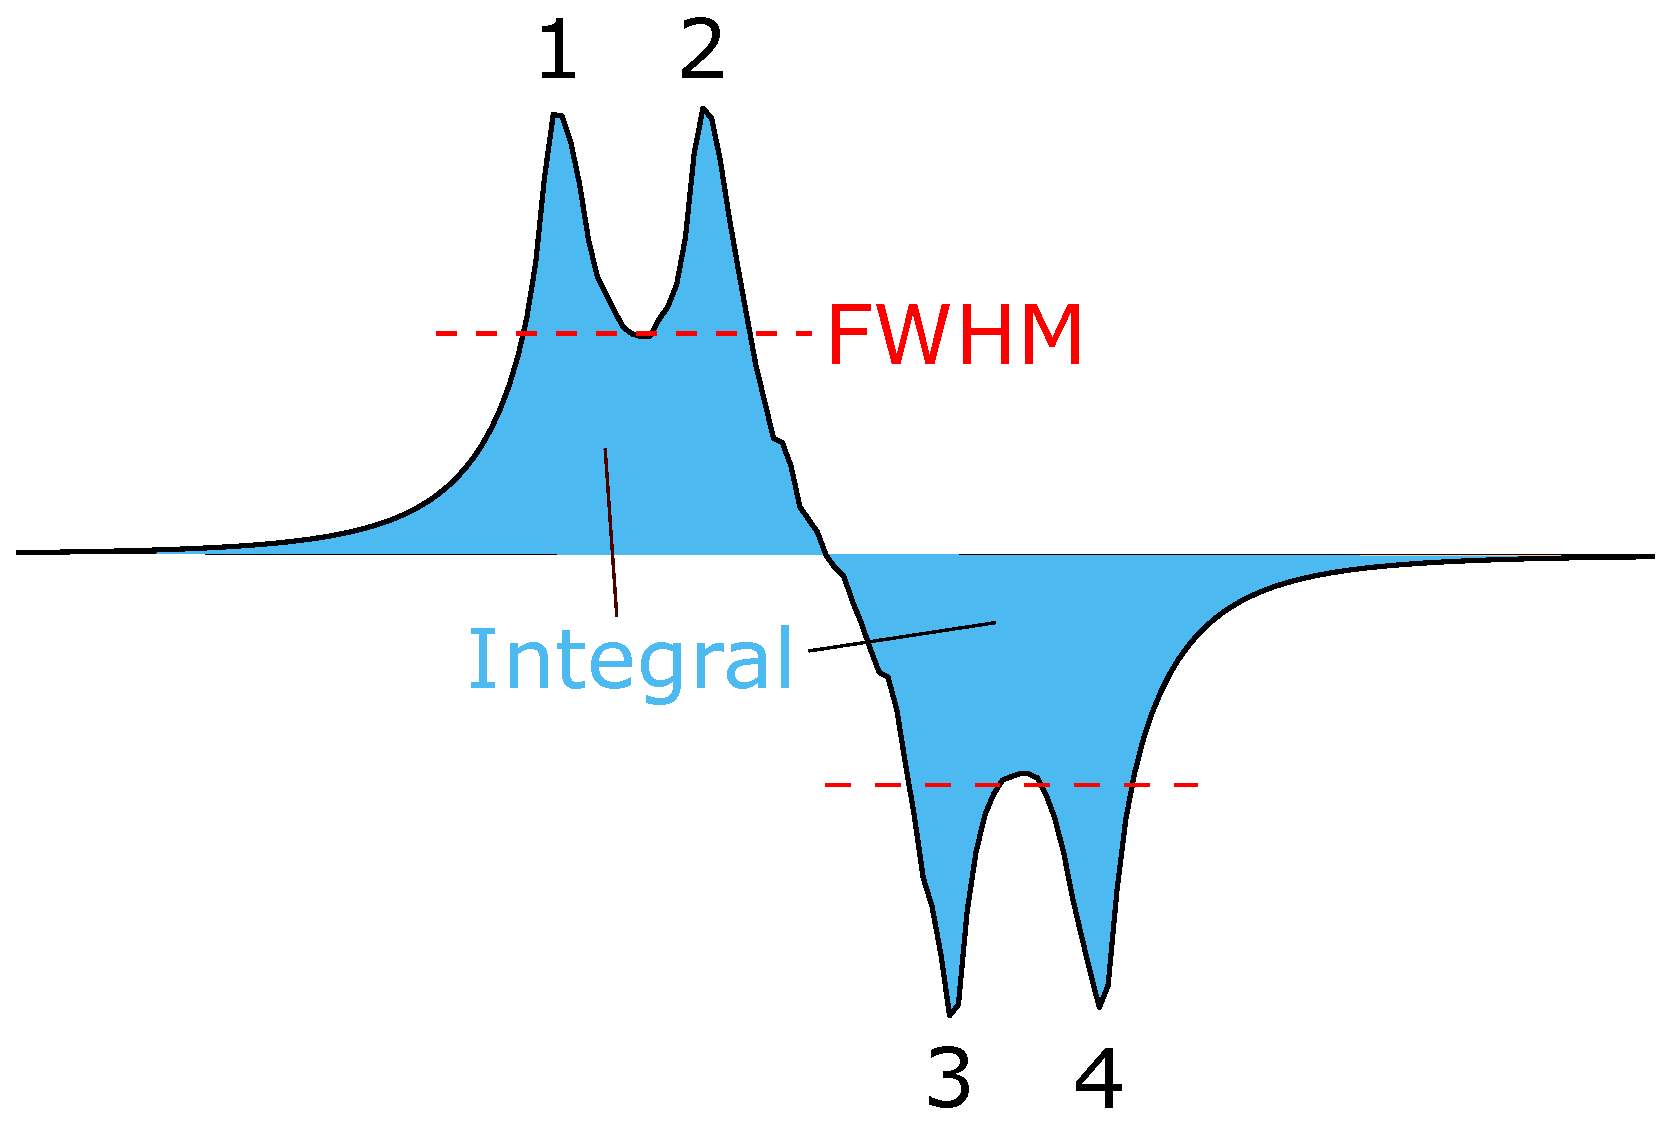
\includegraphics[width=\linewidth,trim={0 0 0 8mm}]{Ressourcen/IMG/ParticleSignalEval}
	\caption{Schematic of a typical signal of two GMR sensors at a distance of \SI{22}{\micro\meter} between them. The red dashes describe the height of the Full Width Half Maximum measurement. Peaks are enumerated to facilitate referencing.}
	\label{fig:sim:peaks}
\end{wrapfigure}
Therefore the .tdms files were at first converted into MATLAB workspace files (.mat) with the help of a premade script from GitHub.\cite{lit:exp:tdms2mat} Afterwards the pre-filtered data was scaled into the zero by subtracting the mean of the whole array from each point. Then, it was filtered by a lowpass filter with a passband frequency of \SI{35}{\Hz} at a sample rate of \SI{10}{\kHz}, infinite impulse response and a transition band steepness of 0.95 ($\in$ [0.5, 1]).

The normal and inverted measurement was browsed for maxima, which were larger than \SI{40}{\percent} of the overall maximum. In the subsequent analysis was searched for peaks in a specific two up, two down pattern by a state-event machine. These patterns were evaluated as for the distance between peaks 12/34, 13, 14 and the distance 4$_{prev}$ to 1$_{next}$ pattern.
The integral of each pattern was computed until the signal dropped to \SI{20}{\percent} of the amplitude. 
%Each finding was plotted against the number of patterns and saved afterward.
\clearpage
\newpage\null\thispagestyle{empty}\newpage
\chapter{Results}
\section{Numerical Simulation Results}
\begin{wrapfigure}[11]{r}{.49\linewidth}
	\centering
	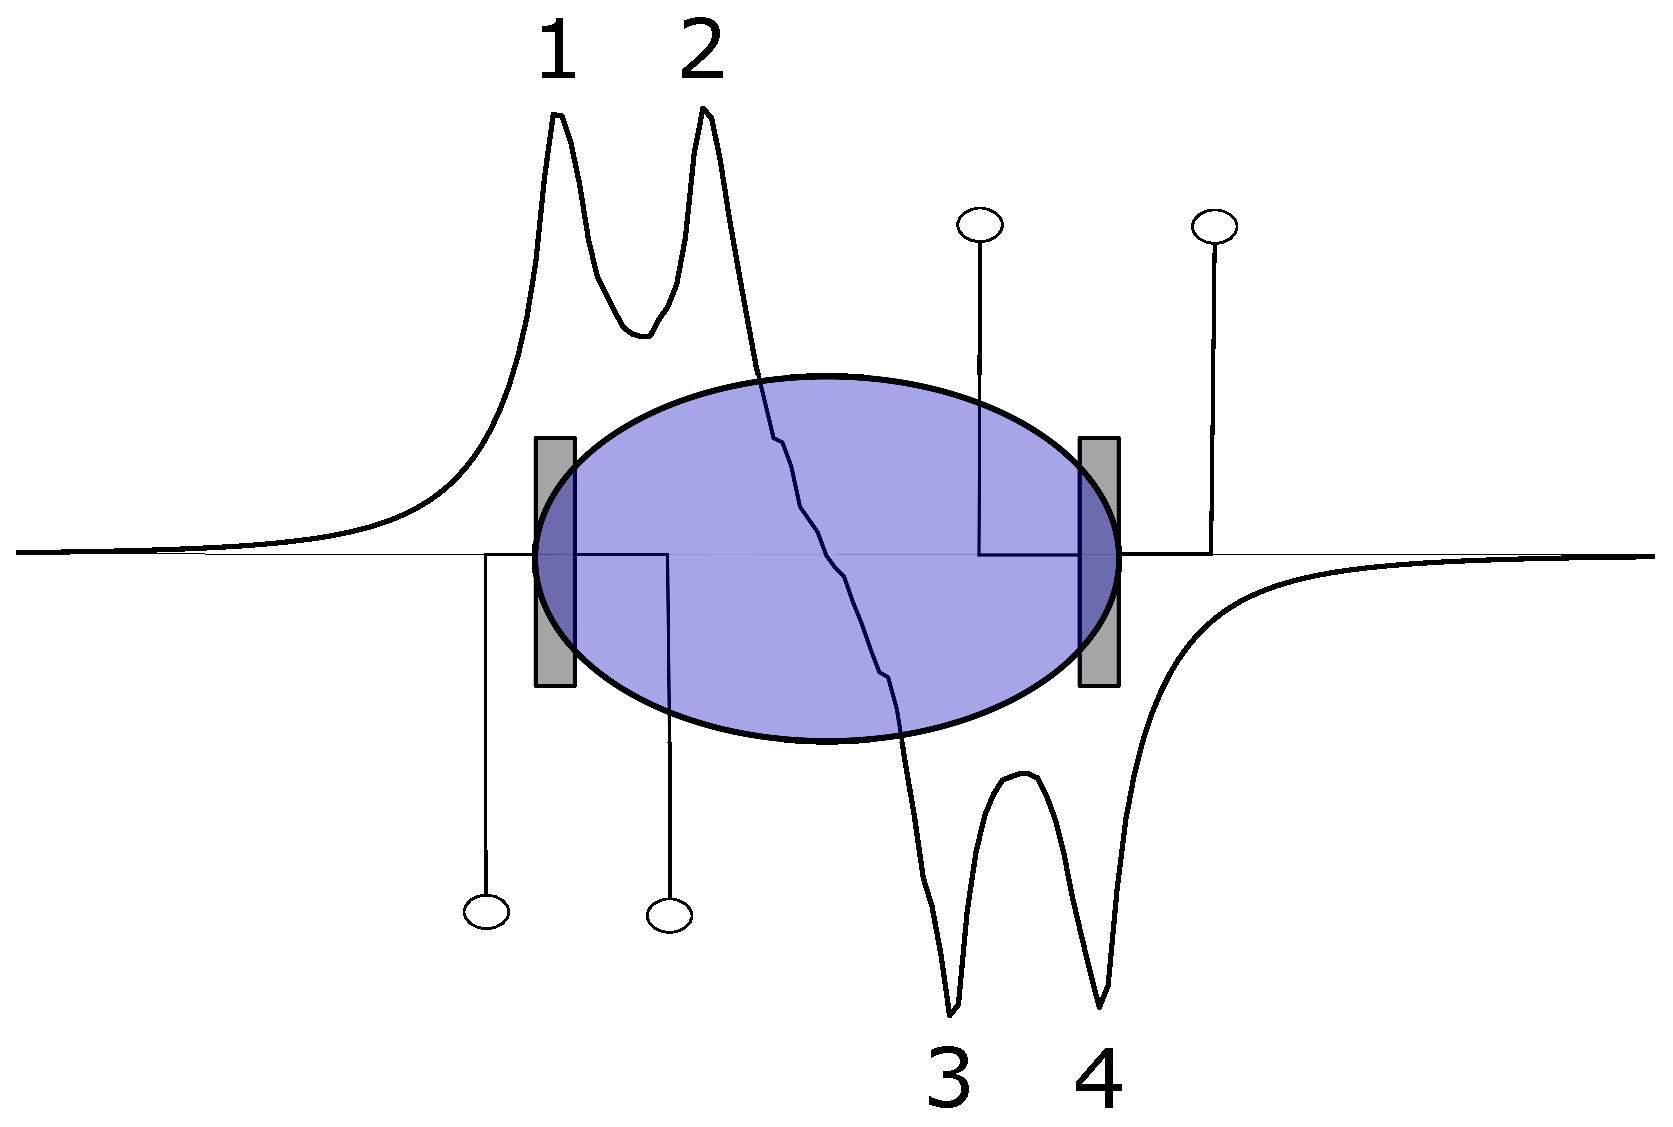
\includegraphics[clip,width=\linewidth]{Ressourcen/IMG/Signal-Bridge}
	\caption{Signal generation at specific droplet positions relatively to the bridge. Both first peaks are generated by the droplet tip, passing each sensor, while the rear peaks are showing the droplet's end passing the half-bridge configuration.}
	\label{fig:res:bridge}
\end{wrapfigure}
The simulation of particles inside the droplets as well as the theoretical signal have both many degrees of freedom, which complicates a useful data evaluation. As a solution, I defined a \acrfull{abbr:spd} with a size of \SI{60}{\micro\meter} length, \SI{40}{\micro\meter} width  and \SI{25}{\micro\meter} height that corresponded to my experimental setup and channel dimensions. An experimentally reachable particle concentration of \SI{e12}{\per\milli\liter} and an offset over the sensor due to passivation and shear forces of \SI{500}{\nano\meter} were also considered as constant values.

\subsection{Superparamagnetic Droplets over single GMR Sensor and Wheatstone Half-Bridge Configuration}
\label{sec:plain_droplets_over_gmr}
At first the comparison of the signal, where a plug flows over a single GMR voltage divider, to a signal, where the plug flows over the Wheatstone half-bridge configuration (\SI{22}{\micro\meter}) was evaluated by varying the different SPD properties.
		\vspace{-5mm}
	\begin{figure}[h!]
	%	\vspace{-5mm}
	\begin{subfigure}[l]{0.49\linewidth} 
		\centering
		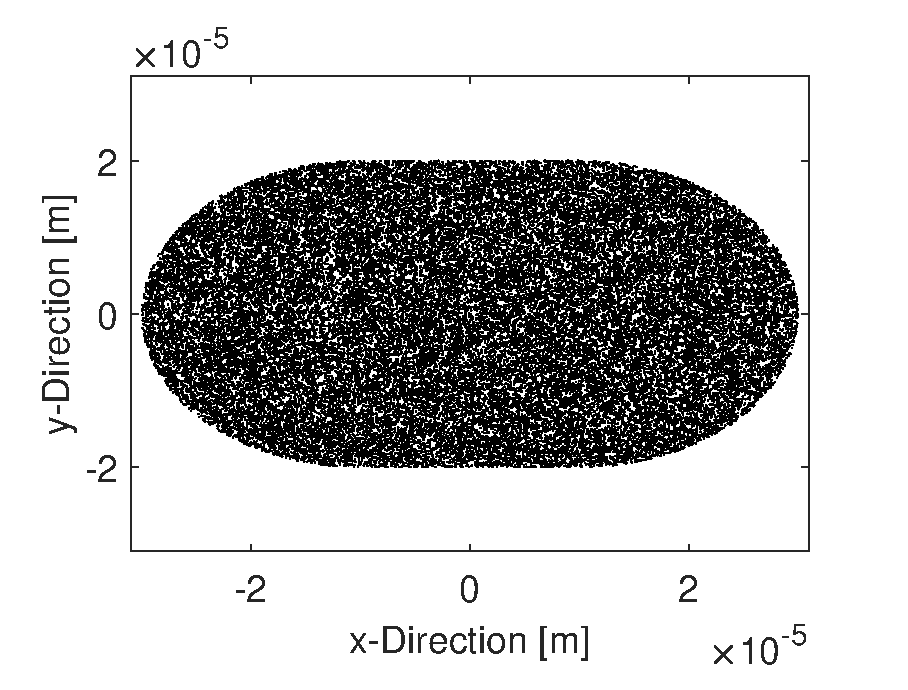
\includegraphics[clip,trim={0mm 0mm 10mm 0mm}, width=\linewidth]{Ressourcen/Results/Top}
		\caption{Particle Distribution inside the Standard Plug Droplet in the x-y-plane}
		\label{fig:sim:SPD:top}
	\end{subfigure}
	\hfil
	\begin{subfigure}[r]{0.49\linewidth} 
		\centering
		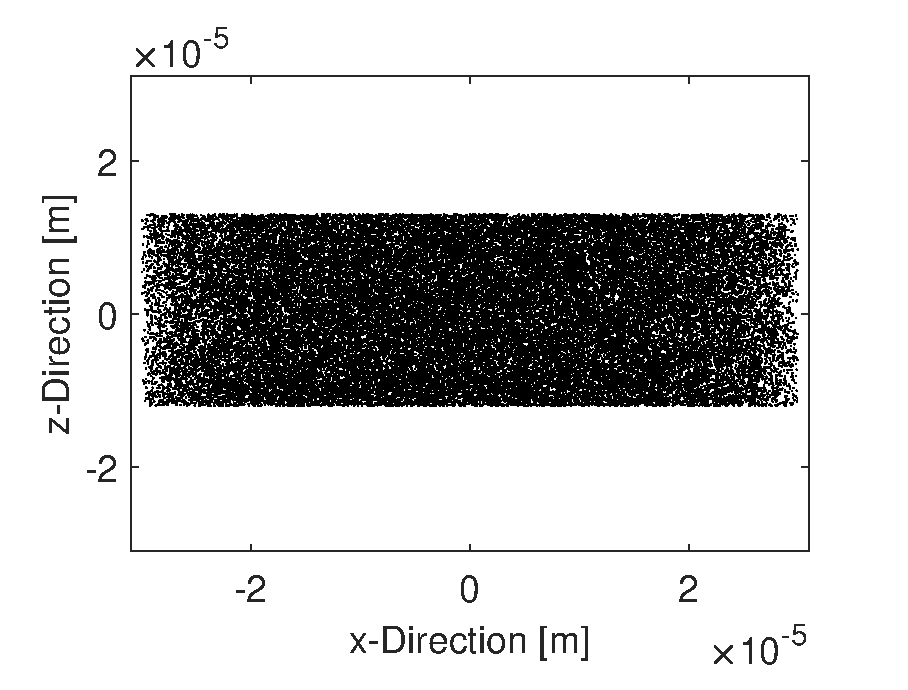
\includegraphics[clip,trim={0mm 0mm 10mm 0mm}, width=\linewidth]{Ressourcen/Results/Side}
		\caption{Particle Distribution inside the Standard Plug Droplet in the x-z-plane}
		\label{fig:sim:SPD:side}
	\end{subfigure}
	\caption{Standard particle distribution of \SI{1E12}{\per\milli\liter}inside a Standard Plug Droplet from two perspectives.}
	\label{fig:sim:SPD}
\end{figure}


Figure \ref{fig:sim:SPD} displays a typical particle distribution inside a droplet for these simulations. Where at the half bridge is a two-up-two-down pattern expected, the single GMR will only produce a single-up-single-down pattern. Because of the comparatively small distance between the two GMRs to the droplet size, an overlap and a loss in information is thereby expected.
\subsubsection{Variation in Droplet Length}
A signal deformation as result of a change in droplet length could be clearly observed in the range around the distance between the sensor elements. That happened due to fact, that the front GMR measured a rising flank, while the rear one already measured a falling flank.\\
\begin{figure}[h]
	\begin{subfigure}[l]{0.49\linewidth} 
		\centering
		\includegraphics[clip,trim={0mm 0mm 0mm 0mm}, width=\linewidth]{Ressourcen/Results/L-400/FWHM}
		\caption{FWHM signal at different droplet lengths}
		\label{fig:sim:l:GMR:FWHM}
	\end{subfigure}
	\hfil
	\begin{subfigure}[r]{0.49\linewidth} 
		\centering
		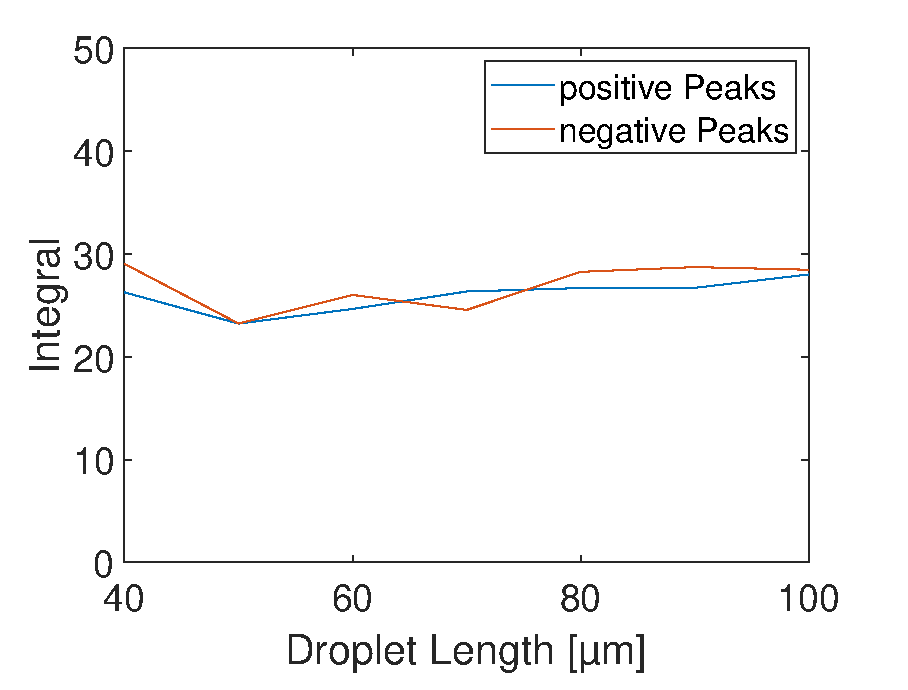
\includegraphics[clip,trim={0mm 0mm 0mm 0mm}, width=\linewidth]{Ressourcen/Results/L-400/Int}
		\caption{Mean of the integrals under each peak at variable droplet lengths}
		\label{fig:sim:l:GMR:int}
	\end{subfigure}
	\vfil
	\begin{subfigure}[r]{0.49\linewidth} 
		\centering
		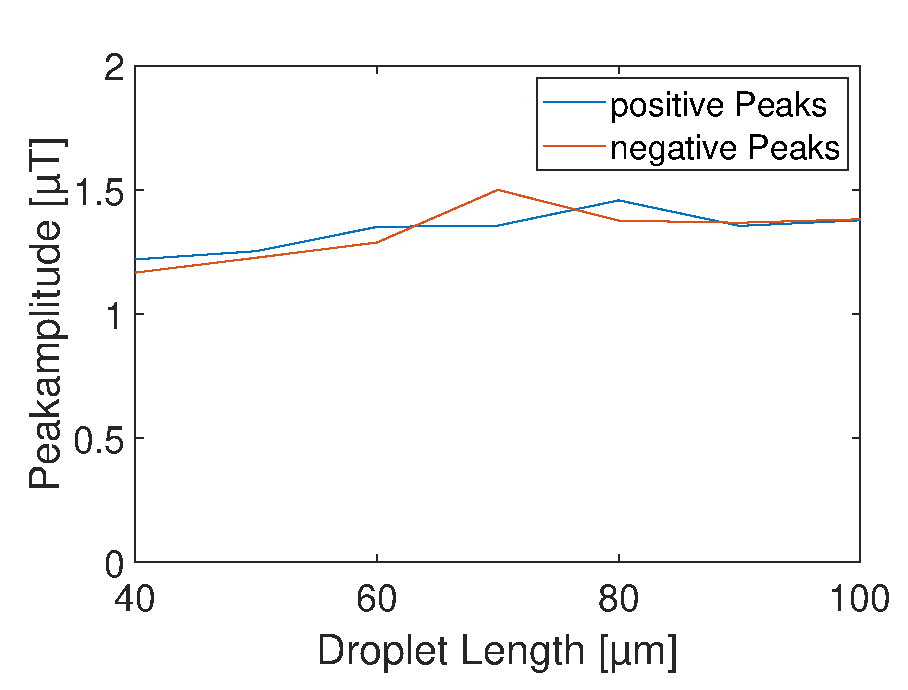
\includegraphics[clip,trim={0mm 0mm 0mm 0mm}, width=\linewidth]{Ressourcen/Results/L-400/Ampl}
		\caption{Peak Amplitude at variable droplet lengths}
		\label{fig:sim:l:GMR:ampl}
	\end{subfigure}
	\hfil
	%	\begin{subfigure}[r]{0.49\linewidth} 
	%		\centering
	%		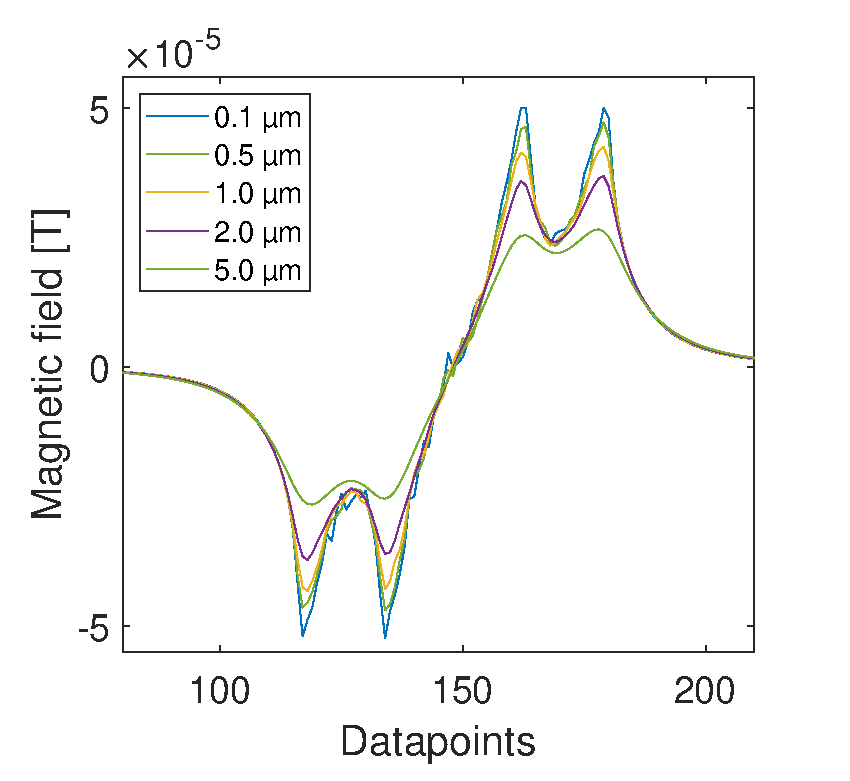
\includegraphics[clip,trim={0mm 0mm 0mm 0mm}, width=\linewidth]{Ressourcen/Results/Shape_Off_z}
	%		\caption{Peak Amplitude at variable particle concentration}
	%		\label{fig:sim:l:shape}
	%	\end{subfigure}
	\caption{Influence of the droplet's length to the simulated signal of a \textbf{single GMR}.}
	\label{fig:sim:l:GMR}
\end{figure}
\newpage
This behavior caused the inner peaks to cancel each other out, resulting in a specific two peak pattern. The lower integral in the beginning of \SIrange{40}{60}{\micro\meter} shows these two instead of four peak patterns. A slight increase with of \acrshort{abbr:fwhm} and integral is also observable at increasing droplet length due to the fact that the slope in the $\pm$ transition of the signal decreases significantly with the droplet width as it lays always by $L_{Droplet}/2$. In order to avoid any inconsistent behavior, the breaking point to linearity at \SI{60}{\micro\meter} was considered therefore as constant droplet length.
\begin{figure}[h]
	\begin{subfigure}[l]{0.49\linewidth} 
		\centering
		\includegraphics[clip,trim={0mm 0mm 0mm 0mm}, width=\linewidth]{Ressourcen/Results/L-22/FWHM}
		\caption{FWHM signal over the Wheatstone bridge}
		\label{fig:sim:l:bridge:FWHM}
	\end{subfigure}
	\hfil
	\begin{subfigure}[r]{0.49\linewidth} 
		\centering
		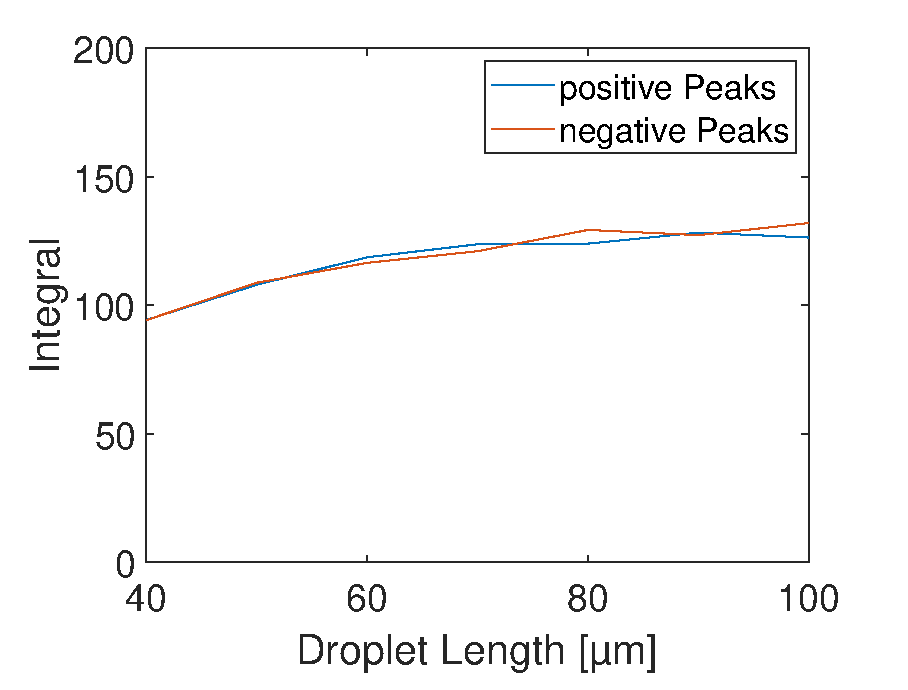
\includegraphics[clip,trim={0mm 0mm 0mm 0mm}, width=\linewidth]{Ressourcen/Results/L-22/Int}
		\caption{Integral of the signal over the Wheatstone bridge}
		\label{fig:sim:l:bridge:int}
	\end{subfigure}
	\vfil
	\begin{subfigure}[r]{0.49\linewidth} 
		\centering
		\includegraphics[clip,trim={0mm 0mm 0mm 0mm}, width=\linewidth]{Ressourcen/Results/L-22/Ampl}
		\caption{Peak amplitude signal for droplets passing the Wheatstone bridge}
		\label{fig:sim:l:bridge:ampl}
	\end{subfigure}
	\hfil
	\begin{subfigure}[r]{0.49\linewidth} 
		\centering
		\includegraphics[clip,trim={0mm 0mm 0mm 0mm}, width=\linewidth]{Ressourcen/Results/L-22/Ampl_in_out}
		\caption{Peak Amplitude of the inner (2,3) and the outer Peaks passing the Wheatstone bridge}
		\label{fig:sim:l:shape}
	\end{subfigure}
	\caption{\textbf{Wheatstone Half-Bridge GMR configuration} with a distance of only \SI{22}{\micro\meter} causes an over-speaking of the falling and rising peaks at small droplet lengths resp. length to width ratios.}
	\label{fig:sim:l:bridge}
\end{figure}
\clearpage
\newpage
\subsubsection{Variation in Droplet Width}
Due to the differential measurement of the GMR system, it was assumed, that an increase in width supports the signal strength to the certain point, where the magnetic field would reach the reference GMRs on either sides. It was then shown in simulation data, that an increasing channel width would enhance the signal quality necessarily by keeping the peaks nearly at a common width but increasing their amplitude to a certain level.
It has to be taken into account, that the simulation lacks for simplification and performance reasons the implementation of such a reference GMR. Another point then would be to move reference resistors far from the channel in order to gain as much signal as possible, while not influencing the differential measurement.
Also, the fact that a droplet's tip changes its radius according to its width supports the broadening of the peaks over width changes.

\begin{figure}[h!]
	\begin{subfigure}[l]{0.49\linewidth} 
		\centering
		\includegraphics[clip,trim={0mm 0mm 0mm 0mm}, width=\linewidth]{Ressourcen/Results/W/W_FWHM}
		\caption{FWHM signal at different droplet widths}
		\label{fig:sim:w:FWHM}
	\end{subfigure}
	\hfil
	\begin{subfigure}[r]{0.49\linewidth} 
		\centering
		\includegraphics[clip,trim={0mm 0mm 0mm 0mm}, width=\linewidth]{Ressourcen/Results/W/W_Int}
		\caption{Peak integrals at variable droplet widths}
		\label{fig:sim:w:int}
	\end{subfigure}
	\vfil
	\begin{subfigure}[r]{0.49\linewidth} 
		\centering
		\includegraphics[clip,trim={0mm 0mm 0mm 0mm}, width=\linewidth]{Ressourcen/Results/W/Ampl}
		\caption{Peak Amplitude at variable droplet widths}
		\label{fig:sim:w:ampl}
	\end{subfigure}
	\hfil
	%	\begin{subfigure}[r]{0.49\linewidth} 
	%		\centering
	%		\includegraphics[clip,trim={0mm 0mm 0mm 0mm}, width=\linewidth]{Ressourcen/Results/Shape_Off_z}
	%		\caption{Peak Amplitude at variable particle concentration}
	%		\label{fig:sim:w:shape}
	%	\end{subfigure}
	\caption{Signal dependency on the droplet width. An overall signal increase in the integral is shown, while the half width stays constant. As a result, signal amplitude increases, which yields in an amplification.}
	\label{fig:sim:w}
\end{figure}
\newpage
\subsubsection{Variation in Droplet Height}
An increasing droplet height causing more MNPs above the sensor seems to result on the one hand side in a gain of amplitude and area below the signal. On the other side, the peaks broaden at growing heights, but go into saturation around \SI{25}{\micro\meter}.\\
This leads to an overall increase in information. However, for the purpose of cell encapsulation, it is necessary to reduce the droplet volume to a minimum in order to prevent movement inside and therefore signal distortion. Consequently, the microfluidic channels were processed at heights between \SIrange{25}{30}{\micro\meter}. 
\begin{figure}[h!]
	\begin{subfigure}[l]{0.49\linewidth} 
		\centering
		\includegraphics[clip,trim={0mm 0mm 0mm 0mm}, width=\linewidth]{Ressourcen/Results/H/FWHM}
		\caption{FWHM signal at different droplet heights}
		\label{fig:sim:h:FWHM}
	\end{subfigure}
	\hfil
	\begin{subfigure}[r]{0.49\linewidth} 
		\centering
		\includegraphics[clip,trim={0mm 0mm 0mm 0mm}, width=\linewidth]{Ressourcen/Results/H/Integral}
		\caption{Peak Amplitude at variable droplet heights}
		\label{fig:sim:h:int}
	\end{subfigure}
	\vfil
	\begin{subfigure}[c]{0.49\linewidth} 
		\centering
		\includegraphics[clip,trim={0mm 0mm 0mm 0mm}, width=\linewidth]{Ressourcen/Results/H/Ampl}
		\caption{Peak Amplitude at variable droplet heights}
		\label{fig:sim:h:ampl}
	\end{subfigure}
	\hfil
%	\begin{subfigure}[r]{0.49\linewidth} 
%		\centering
%		\includegraphics[clip,trim={0mm 0mm 0mm 0mm}, width=\linewidth]{Ressourcen/Results/Shape_Off_z}
%		\caption{Peak Amplitude at variable particle concentration}
%		\label{fig:sim:h:shape}
%	\end{subfigure}
	\caption{Signal shape evaluation in respect of the channel height. Desired signal amplitude (\protect\subref{fig:sim:h:ampl}) and undesired peak breadth (\protect\subref{fig:sim:h:FWHM}) weigh each other out until \SI{25}{\micro\meter}. The integral grows according to the amplitude further, but not with the same slope. Therefore the peaks have to broaden around the lower half maximum (\protect\subref{fig:sim:h:int}).}
	\label{fig:sim:h}
\end{figure}
\newpage

\subsubsection{Variation in Particle Concentration inside the Droplet}
Intuitively, the peak amplitude grows with the particle concentration linearly.  As seen in Figure \ref{fig:sim:conc:ampl}, at low concentrations at the bottom curves the signal is dominated by the fields of single magnetic entities, while the typical two peak pattern is observable at higher concentrations - although distorted due to the logarithmic scale.\\
The first signal without distortions is the yellow one at \num{E12} particles, which was in the latter considered as given value. This parameter was chosen in such a way, because one is able to clearly observe a single entities' signal in the simulation, which will be impossible in a real noisy system.
	\begin{figure}[htb!]
	\begin{subfigure}[l]{0.49\linewidth} 
		\centering
		\includegraphics[clip,trim={0mm 0mm 0mm 0mm}, width=\linewidth]{Ressourcen/Results/Conc/Shape_Conc.eps}
		\caption{Signals of SPD flowing over GMRs with particle concentrations from \SIrange{E9}{E14}{\per\mL} (bottom-up)}
		\label{fig:sim:conc:ampl}
	\end{subfigure}
	\hfil
	\begin{subfigure}[r]{0.49\linewidth} 
		\centering
		\includegraphics[clip,trim={0mm 0mm 0mm 0mm}, width=.9\linewidth]{Ressourcen/Results/Conc/Shape_Conc_Ampl.eps}
		\caption{Peak Amplitude at variable particle concentrations}
		\label{fig:sim:conc:peak}
	\end{subfigure}
	\caption{Linear dependency of peak heights to magnetic particle concentration.}
	\label{fig:sim:conc}
\end{figure}
\newpage

\subsubsection{Vertical Displacement of the whole Droplet}
To study the effect of an offset between droplet and sensor, which could be due to additional passivation or errors in the PDMS-gluing method, the general offset of the whole droplet above the sensor was evaluated. It was shown, that the thickness of the layer has an influence on the signal amplitude, but only little on the peak breadth.\\
The loss of \SI{5}{\micro\tesla\per\micro\meter} from a total amount of  \SI{53.34}{\micro\tesla} causes a signal loss of 9.4\%. A total coating of the Si-chip with the viscous PDMS, which is favorable to build a few micrometer thick layers, therefore is undesirable and was not used.


\begin{figure}[htb!]
	\begin{subfigure}[l]{0.49\linewidth} 
		\centering
		\includegraphics[clip,trim={0mm 0mm 0mm 0mm}, width=\linewidth]{Ressourcen/Results/OffZ/Offset_FWHM}
		\caption{FWHM signal at different offsets above the two GMRs}
		\label{fig:sim:off:z:FWHM}
	\end{subfigure}
	\hfil
	\begin{subfigure}[r]{0.49\linewidth} 
		\centering
		\includegraphics[clip,trim={0mm 0mm 0mm 0mm}, width=\linewidth]{Ressourcen/Results/OffZ/Offset_Int}
		\caption{Peak Amplitude at variable offsets above the GMRs}
		\label{fig:sim:off:z:int}
	\end{subfigure}
\vfil
	\begin{subfigure}[r]{0.49\linewidth} 
	\centering
	\includegraphics[clip,trim={0mm 0mm 0mm 0mm}, width=\linewidth]{Ressourcen/Results/OffZ/Offset}
	\caption{Peak Amplitude at variable offsets above the two GMRs}
	\label{fig:sim:off:z:ampl}
\end{subfigure}
	\hfil
\begin{subfigure}[r]{0.49\linewidth} 
	\centering
	\includegraphics[clip,trim={0mm 0mm 0mm 0mm}, width=\linewidth]{Ressourcen/Results/OffZ/Shape_Off_z}
	\caption{Peak Amplitude at variable offsets above the two GMRs}
	\label{fig:sim:off:z:shape}
\end{subfigure}
	\caption{Signal evaluation at different distances of the droplet above the sensor. The signal shape decreases significantly with higher offsets. In the simulation a critical offset of \SI{5}{\micro\meter} is shown as detection limit. The experimental setup with non-neglectable noise this limit will be lower.}
	\label{fig:sim:off:z}
\end{figure}

\newpage
\subsection{Droplets with Singularity over single GMR}
In the next step, an assumption that the signal would change if a cell or a comparable displacement body was inside a monodisperse droplet, was evaluated. The cell causes a distortion in the droplet pattern described in \ref{sec:plain_droplets_over_gmr}, especially if it is stained with magnetic beads. I could show, that the signal depends on the diameter, position and amount of beads on the cell's surface. Furthermore, the simulation gave an insight, how the measurement data depends on the size of the droplet in relation to the singularity dimensions. \\
The standardized droplet for comparable data generation was again the SPD, but with the alteration of a singularity inside with radius \SI{6}{\micro\meter}. On the surface, there were different coverage percentages possible from 0-100\%. The minimal and maximal coverage are displayed in the pictures below.
	\begin{figure}[htb!]
	\begin{subfigure}[l]{0.49\linewidth} 
		\centering
		\includegraphics[clip,trim={0mm 0mm 0mm 0mm}, width=\linewidth]{Ressourcen/Results/Singularity/Side-empty}
		\caption{Side-view of a \acrshort{abbr:spd} with a \SI{6}{\micro\meter} Singularity and no particles on the outside.}
		\label{fig:sim:singularity:drop:empty}
	\end{subfigure}
	\hfil
	\begin{subfigure}[r]{0.49\linewidth} 
		\centering
		\includegraphics[clip,trim={0mm 0mm 0mm 0mm}, width=\linewidth]{Ressourcen/Results/Singularity/Side-full}
		\caption{Side-view of a \acrshort{abbr:spd} with a \SI{6}{\micro\meter} Singularity fully covered with particles on the outside.}
		\label{fig:sim:singularity:drop:full}
	\end{subfigure}
	\caption{Particle distributions inside a SPD with a simulated cell inside. The singularity's radius is \SI{6}{\micro\meter}. The left figure displays cell, which is not labeled, while the right plot shows a cell, which is 100\% covered with magnetic particles.}
	\label{fig:sim:singularity:drop}
\end{figure}

However, due to the overlap of both two positive and two negative peaks, the signal could not be evaluated with the conventional half-bridge setup. Hence, for the whole singularity simulation, the two spin valves have been separated by a multiple of the droplet length and the signals have been considered as single ones.
\newpage
\subsubsection{Results for Singularities inside the Droplet with and without MNPs attached}
Due to the laminar flow, spontaneous mixing inside the droplets is unlikely. This causes the cells to stay at their position, where they have been encapsulated. Shrinking the droplet volume enhances on the one hand side the overall volume, which is covered by the cell, and on the other side the likelihood of a centered cell inside. \\
In the first analysis, it was evaluated whether a magnetic labeling could generate a higher sensitivity for instance. Figure \ref{fig:sim:encapsulation:signal} shows a singularity with \SI{12}{\micro\meter} radius at a droplet's center (0,0,0) with variable MNP coverages (0\%,25\%,50\%,75\%,100\%).

\begin{figure}[h]
	\centering
	\includegraphics[page=2,clip,trim={0mm 0mm 0mm 0mm},width=\linewidth]{Ressourcen/Results/Singularity/Cell_Encapsulation}
	\caption{Signal dependency on magnetic labeling of a cell: Pattern shapes at different surface coverage rates (shown in the cake diagram) from 0 - 100\%.}
	\label{fig:sim:encapsulation:signal}
\end{figure}

The singularity generates an opposing peak pattern due to the differential measurement, which grows also linearly with the particle coverage (as shown in \ref{fig:sim:conc}). Thereby, a perfectly centered singularity does not interfere with the two surrounding peaks from the droplet itself. It is easily inferable, that a singularity near the tips causes a height distortion of either outer peaks. \\
Interestingly, also an empty singularity as depicted in the top-left corner can be measured in the signal. This is likely based on the redistribution of MNPs outside the cell, forcing an empty volume with no magnetism. A coverage rate of 25\% is close to the base particle concentration in the dispersed phase and displays therefore not detectable spikes.
\newpage
The generated patterns have been analyzed over the established parameters (Fig. \ref{fig:sim:singularity:peak_eval}). As already mentioned, the peaks of the droplet itself are not influenced by the particle coverage.
The uncommon function of in topology used prominence is taken into account now. The prominence of a peak is the minimum height necessary to descend to get from the tip to any higher peaks. The prominence therefore grows until the inner peak outgrows the outer one and then decreases as the algorithm detects only a two peak pattern again.
\\
A correlation between the other two parameters (FWHM and integral) is also shown, but not necessary for the signal analysis. As discussed, the integral is at constant amplitude only determined by the FWHM, which is observable in the lower plots and depicts the same properties in poorer quality as the peak prominence.
\begin{figure}[htb!]
	\begin{subfigure}[l]{0.49\linewidth} 
		\centering
		\includegraphics[clip,trim={0mm 0mm 0mm 0mm}, width=\linewidth]{Ressourcen/Results/Singularity/ampl}
		\caption{Amplitude analysis of the two peaks.}
		\label{fig:sim:singularity:ampl}
	\end{subfigure}
	\hfil
	\begin{subfigure}[r]{0.49\linewidth} 
		\centering
		\includegraphics[clip,trim={0mm 0mm 0mm 0mm}, width=\linewidth]{Ressourcen/Results/Singularity/prom}
		\caption{Prominence of a single peak.}
		\label{fig:sim:singularity:prom}
	\end{subfigure}
	\vfil
	\begin{subfigure}[r]{0.49\linewidth} 
		\centering
		\includegraphics[clip,trim={0mm 0mm 0mm 0mm}, width=\linewidth]{Ressourcen/Results/Singularity/fwhm}
		\caption{FWHM evaluation of a pattern}
		\label{fig:sim:singularity:fwhm}
	\end{subfigure}
	\hfil
	\begin{subfigure}[r]{0.49\linewidth} 
		\centering
		\includegraphics[clip,trim={0mm 0mm 0mm 0mm}, width=\linewidth]{Ressourcen/Results/Singularity/int}
		\caption{Integral under each peak.}
		\label{fig:sim:singularity:int}
	\end{subfigure}
	\caption{Signal evaluation at different singularity coverages in a droplet's center. While the overall amplitude of the peak's is not influenced, peak width, prominence and integral show a subordination on the particles on a cell's surface.}
	\label{fig:sim:singularity:peak_eval}
\end{figure}
\newpage
\subsubsection{Dependency of Magnetic Signal on the Position of Singularity inside a Droplet}
\begin{wrapfigure}[8]{r}{0.5\linewidth}
	\centering
	\includegraphics[page=1,clip,trim={10mm 30mm 35mm 30mm},width=\linewidth]{Ressourcen/Results/Singularity/Cell_Encapsulation}
	\caption{Schematic of simulation positions of a cell inside a droplet in the x-z-plane and a single spin valve underneath.}
	\label{fig:sim:encapsulation:pos}
\end{wrapfigure}
Another evaluation parameter was the position of the cell inside the droplet. I defined several assessment positions based on probability densities of the cell as drawn in the schematic on the right. What was assumed beforehand, was now confirmed through the different signal shapes (Figure \ref{fig:sim:singularity:signal}). \\A shift towards any tip of the droplet increases its amplitude, while contrarily enforcing a single peak in the pattern's center. Additionally, the height inside the SPD plays an important role for this analysis. The red and purple curves depict both a singularity centered in the very front of the tip, but the red one is also shifted to the top, whereas the purple stays in the center. A significant decrease of \SI{2}{\micro\tesla} can be observed in this case.\\
A differentiation between the shift in x-direction is also possible, regarding the centered peaks sign and position. The relation between the blue and purple line is a difference of \SI{8}{\micro\meter} throughout the droplet length. A slightly differing height is observable, but moreover a great shift of the centered peaks.
\begin{figure}[h]
	\centering
	\includegraphics[clip,trim={55mm 20mm 50mm 10mm},width=\linewidth]{Ressourcen/Results/Singularity/r=6,part+pos=var}
	\caption{Signal dependency on the position of the cell inside the droplet at constant diameter of \SI{12}{\micro\meter} and particle coverage of 100\%.}
	\label{fig:sim:singularity:signal}
\end{figure}



\section{Experimental Results}
\subsection{Parameter Evaluation of Droplet Generation}
The parameters obtained from the numerical simulation were now tested under real conditions in the described microfluidics systems and with optical correlation. In fact, a proof of concept could be developed and effective settings for pump flow rates and sensor supply be established. Because of the dependency of the flow to the channel dimensions for different geometries from \SIrange{30}{50}{\micro\meter}, it was found that flow rates around \SI{1}{\nano\liter\per\second} in the mentioned relation have been sufficient for a stable droplet flow with the desired sizes. At higher flow rates, the integrator inside the Lock-In-Amp, which acts as a lowpass filter, would not be able to recover a correct signal, whilst the pump system could not manage lower flow rates than \SI{0.1}{\nano\liter\per\second}, which could not diminish the droplet speed further. In essence, a perfect setup for a \SI{40}{\micro\meter} channel would consist out of \SI{0.5}{\nano\liter\per\second} $Q_c$ and \SI{0.3}{\nano\liter\per\second} $Q_d$, where the bridge was supplied with \SIrange{250}{400}{\mV} at a \SIrange{50}{25}{\kHz} sinusoidal voltage.

Another parameter to be assessed in the beginning has been the concentration of nanoparticles matched to the real signal resp. SNR or RMS in comparison to the simulation. At first, the concentration was set to a fixed value of \SI{E12}{\particle\per\ml}. This brought at a particle diameter of \SI{50}{\nm} a SNR of 3 - 5 dependent on the bridge quality. A lower detection limit could not be found due to the contamination of the continuous phase with dust, which obstructed the channels regularly and prevented qualitative data for significant analysis. Furthermore, a very light adhesion of the PDMS to the \acrfull{abbr:sin} on the surface caused multiple times a tear-off.\\
Also, a comparison to \SI{2}{\micro\meter} beads was set up, but could not be significantly investigated due to the mentioned problems. However, I observed the typical up-down-up-down pattern as described in \cite{lit:Bojan} during single droplet measurements with the bigger particles.

\newpage

\subsection{Optical Tracking and Validation of Droplet Length and Velocity}
                        
                        \vspace{1cm}
	\begin{figure}[h]
	\begin{subfigure}[l]{0.49\textwidth} 
		\centering
		\includegraphics[clip,trim={0mm 0mm 0mm 0mm}, scale=.5]{Ressourcen/Tracking/Length}
		\caption{Discrete Ellipse Major Axes (corresponding to the droplet length) in each frame}
		\label{fig:tracking:length}
	\end{subfigure}
	\hfil
	\begin{subfigure}[r]{0.49\textwidth} 
		\centering
		\includegraphics[clip,trim={0mm 0mm 0mm 0mm},scale=.5]{Ressourcen/Tracking/Width}
		\caption{Discrete Ellipse Minor Axes (corresponding to the droplet width) in each frame.}
		\label{fig:tracking:width}
	\end{subfigure}
\vfil
	\begin{subfigure}[l]{0.49\textwidth} 
	\centering
	\includegraphics[clip,trim={0mm 0mm 0mm 0mm}, scale=.5]{Ressourcen/Tracking/HistogramLength}
	\caption{Distribution of major ellipse axes over the analyzed frames.}
	\label{fig:tracking:histLength}
\end{subfigure}
\hfill
\begin{subfigure}[r]{0.49\textwidth} 
	\centering
	\includegraphics[clip,trim={0mm 0mm 0mm 0mm},scale=.5]{Ressourcen/Tracking/HistogramWidth}
	\caption{Distribution of minor axes over analyzed frames with a Gaussian fit (red).}
	\label{fig:tracking:histWidth}
\end{subfigure}
	\caption{Measurement at a flow rate of \SI{10}{\micro\liter}(Q$_c$) to \SI{4}{\micro\liter}(Q$_d$), which was dropped at half of the time to \SI{2}{\micro\liter}(Q$_d$). Discrete values computed by the algorithm are shown above (\protect\subref{fig:tracking:length},\protect\subref{fig:tracking:width}), a decrease in width accuracy at smaller droplet lengths can be observed. The figures below show the distribution of each parameter (\protect\subref{fig:tracking:histLength},\protect\subref{fig:tracking:histWidth}). For the length two populations can be clearly observed. Maxima can be obtained by Gaussian fits. The extremum of the red fit in \protect\subref{fig:tracking:width} lies at 17.69, because of the fact, that the algorithm is designed to find the inner ellipse of a droplet's edge. This issue can be observed also in figure \ref{fig:tracking:livefitting}.}
	\label{fig:tracking:dims}
\end{figure}

To determine a reference for the correct signal evaluation and remove the undesired dependency of the peaks to velocity and droplet dimensions, the MATLAB tracking of a microscope captured video was analyzed in figures \ref{fig:tracking:dims} and \ref{fig:tracking:movement}. As test for the algorithm, flow rates were changed at half of the measurement interval. The script clearly finds two populations of droplet lengths, while the width analysis is suffering from the inaccuracy of image edge detection.
\newpage
However, in the sum the program convolves to a mean width of \SI{17.89}{\micro\meter} because of very large edges at the sides in microscope images. Lower aperture and more intense light settings decreased this problem. The displayed length (Fig. \ref{fig:tracking:length}) has a specific positive slope for the reason of droplet deformation after the pinch-off before its terminal orientation inside the channel.

The velocity evaluation showed also the expected results, where the frame rate multiplied with the center movement of the fitted ellipse gave the velocity. The droplets at higher flow rates showed therefore a higher velocity around \SI{2.94}{\mm\per\second} and the longer droplets a mean velocity of \SI{1.78}{\mm\per\second}. 
\begin{figure}
	\begin{subfigure}[l]{0.49\textwidth} 
	\centering
	\includegraphics[clip,trim={0mm 0mm 0mm 0mm}, scale=.5]{Ressourcen/Tracking/LocationDropletCenter}
	\caption{Movement of the mean droplet center position in regards to the image acquisition time of 4.5 s.}
	\label{fig:tracking:center}
\end{subfigure}
\hfill
\begin{subfigure}[r]{0.49\textwidth} 
	\centering
	\includegraphics[clip,trim={0mm .5mm 0mm 0mm},scale=.49]{Ressourcen/Tracking/Velocity}
	\caption{Distribution of droplet velocities per frame.}
	\label{fig:tracking:velocity}
\end{subfigure}
\caption{On the left hand side, the absolute movement of the averaged center of the six fitted ellipses per frame shows that the relative distance between each point increases for shorter droplets (as seen in Fig. \ref{fig:tracking:dims}). Diagram 	\protect\subref{fig:tracking:velocity} expresses the distribution of resulted velocities per frame.}
\label{fig:tracking:movement}
\end{figure}
\newpage


\subsection{Magnetoresistive Characterization of Droplets in Wheatstone Half-Bridge Configuration}

\begin{figure}[h]
	\begin{subfigure}[c]{\textwidth} 
		\centering
		\includegraphics[clip,trim={35mm 0mm 35mm 7mm}, width=\linewidth]{Ressourcen/Results/Measurement/Raw}
		\caption{Complete droplet measurement stream at a flow rates of \SI{9}{\nano\liter}(Q$_c$) to \SI{6}{\nano\liter}(Q$_d$) with filtered signal and applied peak evaluation.}
		\label{fig:exp:raw}
	\end{subfigure}
	\vfill
	\begin{subfigure}[l]{.49\textwidth} 
		\centering
		\includegraphics[clip,trim={0mm .5mm 0mm 0mm},width=\linewidth]{Ressourcen/Results/Measurement/Raw_in}
		\caption{Zoom into characteristic 2-hi-2-lo pattern-sequences of the measured signal.}
		\label{fig:exp:peaks}
	\end{subfigure}
	\hfill
\begin{subfigure}[r]{.49\textwidth} 
	\centering
	\includegraphics[clip,trim={0mm .5mm 0mm 0mm},width=\linewidth]{Ressourcen/Results/Measurement/Pattern}
	\caption{Evaluated, filtered pattern of one droplet with integral to 20\% amplitude.}
	\label{fig:exp:pattern:raw}
\end{subfigure}
	\caption{Typical measurement signal at different magnification for a monodisperse droplet generation at pump rates of \SI{9}{\nano\liter}(Q$_c$) and \SI{6}{\nano\liter}(Q$_d$) with evaluation integral and peak detection.}
\end{figure}

The measured signal, displayed in the upper figure, was also evaluated for its properties such as amplitude, peak distances, FWHM and integral under each peak. Furthermore, an estimation to the droplet velocity was computed from the distance of the upper peaks. The height of each of the four peaks was assessed for stability over the signal. It can be observed in figure \ref{fig:exp:pattern:height} that the leading positive peaks are almost \SI{0.1}{\mV} less than the negative peaks. A possible explanation is maybe the form of a droplet in the stream. The differential measurement method detects minimal changes in the tip radius sensitively, which then increases the amplitude. Another explanation could be the non-centered channel over the GMR sensors, which causes an asymmetry of the magnetic field's y-compounds and therefore an anisotropy field in one direction that causes lower amplitude for only positive or negative angles of the free layer.

\begin{figure}
	\begin{subfigure}[l]{0.49\textwidth} 
		\centering
		\includegraphics[clip,trim={0mm 0mm 0mm 0mm}, width=1.1\linewidth]{Ressourcen/Results/Measurement/Height_abs}
		\caption{Measured mean peak voltage at each pattern for positive and negative peaks.}
		\label{fig:exp:pattern:height:abs}
	\end{subfigure}
	\hfill
	\begin{subfigure}[r]{0.49\textwidth} 
		\centering
		\includegraphics[clip,trim={0mm 0mm 0mm 0mm}, width=1.05\linewidth]{Ressourcen/Results/Measurement/Height_hist}
		\caption{Statistical evaluation of positive and negative peak amplitudes.}
		\label{fig:exp:pattern:height:hist}
	\end{subfigure}
	\caption{Peak amplitude analysis in respect to the mean of each both positive and negative peaks.}
	\label{fig:exp:pattern:height}
\end{figure}

In the mean of distances of Peaks 12 and 34, it was tried to gain an insight into the mean velocity of a single droplet over time. As large-signal, a single negative oscillation can be measured, which is caused by the step-wise pumping of the syringe system at small flow rates. In the scatter plot (\protect\ref{fig:exp:pattern:vel:amp}), a slightly decreasing signal amplitude at growing velocities is shown, which is also relatable to the slow lowpass in the signal processing.\\
Also the speed's discrepancy of nearly one decade is influenced by the syringe system and the measurement technique itself. Due to the fact, that the spin valve is influenced by the magnetic field lines already in front and still in the back of a droplet, exact measurements are unlikely. 

\begin{figure}[h]
	\begin{subfigure}[l]{0.49\textwidth} 
		\centering
		\includegraphics[clip,trim={0mm 0mm 0mm 0mm}, width=1.1\linewidth]{Ressourcen/Results/Measurement/Vel_12}
		\caption{Velocities at each 4-peak-pattern in the signal.}
		\label{fig:exp:pattern:vel:12}
	\end{subfigure}
	\hfill
	\begin{subfigure}[r]{0.49\textwidth} 
		\centering
		\includegraphics[clip,trim={0mm 0mm 0mm 0mm}, width=1.1\linewidth]{Ressourcen/Results/Measurement/Vel-Amp}
		\caption{Signal amplitude change over the range of droplet velocities.}
		\label{fig:exp:pattern:vel:amp}
	\end{subfigure}
	\caption{Velocity evaluation of droplets by comparing the distance between the bridge resistors (\SI{22}{\micro\meter}) to time interval between the peaks.}
\end{figure}
\clearpage

Below, the raw data for a calculation of a droplet's velocity is displayed with its distribution on the right side (Fig. \ref{fig:exp:pattern:1234}). Besides the three artifacts in figure \ref{fig:exp:pattern:12:abs}, a saw tooth trace from the pump oscillation is again visible. The velocity (thus the pressure) decreases until the maximum, when the pump starts another stroke and the pressure rapidly increases. \\
Another discovery from these data is that the positive and negative peaks have apart from their different amplitude the same distances over time. This leads to the finding that the shape of a droplet has to be symmetric in its tips, but not necessarily the particle distribution inside.

\begin{figure}[h]
	\begin{subfigure}[l]{0.49\textwidth} 
		\centering
		\includegraphics[clip,trim={0mm 0mm 0mm 0mm}, width=1.1\linewidth]{Ressourcen/Results/Measurement/12_34_abs}
		\caption{Pairwise Distance between both positive and negative peaks at each 4-peak-pattern in the signal.}
		\label{fig:exp:pattern:12:abs}
	\end{subfigure}
	\hfill
	\begin{subfigure}[r]{0.49\textwidth} 
		\centering
		\includegraphics[clip,trim={0mm 0mm 0mm 0mm}, width=1.1\linewidth]{Ressourcen/Results/Measurement/12_34_hist}
		\caption{Peak distance change over the range of droplet velocities.}
		\label{fig:exp:pattern:12:hist}
	\end{subfigure}
%\vfil
%	\begin{subfigure}[l]{0.49\textwidth} 
%	\centering
%	\includegraphics[clip,trim={0mm 0mm 0mm 0mm}, width=1.1\linewidth]{Ressourcen/Results/Measurement/34_abs}
%	\caption{Pairwise Distance between 34 at each 4-peak-pattern in the signal.}
%	\label{fig:exp:pattern:34:abs}
%\end{subfigure}
%\hfill
%\begin{subfigure}[r]{0.49\textwidth} 
%	\centering
%	\includegraphics[clip,trim={0mm 0mm 0mm 0mm}, width=1.1\linewidth]{Ressourcen/Results/Measurement/34_hist}
%	\caption{Peak distance change over the range of droplet velocities.}
%	\label{fig:exp:pattern:34:hist}
%\end{subfigure}
	\caption{Velocity evaluation of droplets by comparing the distance between the bridge resistors (\SI{22}{\micro\meter}) to time interval between the peaks. Numerical instabilities of MATLAB cause singularities in Peak 34 (Fig. \protect\subref{fig:exp:pattern:12:abs}). Saw-tooth-like pump oscillation, but also similarities in the distances of positive and negative patterns are visible.}
	\label{fig:exp:pattern:1234}
\end{figure}
Next, there was also the mean integral under each pattern regarded. Assuming a linear dependency on FWHM and amplitude, it can be inferred that FWHM is the domination factor in this relation. Following this, the peaks broaden at lower velocities. The velocity-normalized plot (Figure \ref{fig:exp:pattern:integral}) shows a constant peak width in relation to its velocity. The DAQ-card encodes more data-points per droplet at smaller speeds, which results in smaller slopes of the flanks but remaining the same amplitude.
\clearpage
To get information about a droplet's length, while it is passing the sensing element, the distance between peak 1 and 3 respectively peak 1 and 4 minus the sensor element distance has been also measured (Figure \ref{fig:exp:pattern:13}). The problem of magnetic stray fields outside a plug persists as in the velocity computation.

\begin{figure}[h]
	\vspace{-10px}
	\begin{subfigure}[l]{0.49\textwidth} 
		\centering
		\includegraphics[clip,trim={0mm 0mm 0mm 0mm}, width=1.1\linewidth]{Ressourcen/Results/Measurement/Int.eps}
		\caption{Mean integral under each pattern normalized by the droplet velocity.}
		\label{fig:exp:pattern:integral}
	\end{subfigure}
	\hfill
	\begin{subfigure}[r]{0.49\textwidth} 
		\centering
		\includegraphics[clip,trim={0mm 0mm 0mm 0mm}, width=\linewidth]{Ressourcen/Results/Measurement/13_14_abs}
		\caption{Velocity corrected Distance of Peak 13 and Peak 14 - \SI{22}{\micro\meter} in each pattern}
		\label{fig:exp:pattern:13}
	\end{subfigure}
	\caption{(\protect\subref{fig:exp:pattern:integral}) Mean absolute integral under each pattern. Droplet length evaluation by comparing the distance between the bridge resistors (\SI{22}{\micro\meter}) to time interval between the peaks 13 and (peaks 14 - \SI{22}{\micro\meter}). The data is normalized to the previously calculated velocity.}
\end{figure}
Nevertheless, the data shows the expected outcome, where a droplet's length increases during a pumping oscillation, because the more viscous oil phase transfers apparently pumping oscillations more facile than the water phase. A normalization to the velocity as applied, corrects again the pump oscillations and shows a quadratic behavior on the pressure inside the channel.

\begin{figure}[h!]
	\begin{subfigure}[l]{0.49\textwidth} 
		\centering
		\includegraphics[clip,trim={0mm 0mm 0mm 0mm}, width=1\linewidth]{Ressourcen/Results/Measurement/FWHM_abs}
		\caption{Absolute mean Full Width at Half Maximum over every peak in all patterns normed by velocity.}
		\label{fig:exp:pattern:FWHM:abs}
	\end{subfigure}
	\hfill
	\begin{subfigure}[r]{0.49\textwidth} 
		\centering
		\includegraphics[clip,trim={0mm 0mm 0mm 0mm}, width=1\linewidth]{Ressourcen/Results/Measurement/FWHM_hist}
		\caption{Distribution of Full Width at Half Maximum with Gaussian fit (red) in all patterns.}
		\label{fig:exp:pattern:FWHM:hist}
	\end{subfigure}
	\caption{Signal breadth evaluation by performing a Full Width at Half Maximum analysis of each peak and depicting the absolute mean of each pattern (\protect\ref{fig:exp:pattern:FWHM:abs}) and its Gaussian distribution (\protect\ref{fig:exp:pattern:FWHM:hist}).}
	\label{fig:exp:pattern:FWHM}
\end{figure}
\clearpage
Furthermore, the mentioned Full Width at Half Maximum (FWHM) has been also analyzed (Figure \ref{fig:exp:pattern:FWHM}). On the one hand side, FWHM states how low or high frequent a signal component is, which has influence on the used filter. Low frequency of the desired signal allows a smaller cutoff frequency and therefore to remove more noise from the signal while simultaneously maintaining more original shape. On the other side, its roughly linear relation to the integral and amplitude demonstrates the goodness of a signal resp. spin valve. \\
As described before, the peak width contributes mainly to the integral shape as well the distance measurements. Hence, it represents a valuable parameter for signal analysis condensing many information from the graphs above. 


Lastly, the complete distance between each pattern was measured by the difference of the last peak of the former pattern to the first peak of the next pattern: \\ 
Distance~=~Time$_{Peak 1, next}$~-~Time$_{Peak 4, prev}$. The pumping oscillation can also be observed. However, the slope is shallower as in the other graphs guiding the hypothesis of stray fields, which decrease the absolute signal quality. 

\begin{figure}[h]
	\begin{subfigure}[l]{0.49\textwidth} 
		\centering
		\includegraphics[clip,trim={0mm 0mm 0mm 0mm}, width=1.1\linewidth]{Ressourcen/Results/Measurement/Dist_abs}
		\caption{Absolute distance between peak 4 of the previous and peak 1 of the next pattern.}
		\label{fig:exp:pattern:Dist:abs}
	\end{subfigure}
	\hfill
	\begin{subfigure}[r]{0.49\textwidth} 
		\centering
		\includegraphics[clip,trim={0mm 0mm 0mm 0mm}, width=1.1\linewidth]{Ressourcen/Results/Measurement/Dist_hist}
		\caption{Distribution of two consecutive patterns with Gaussian fit (red).}
		\label{fig:exp:pattern:Dist:hist}
	\end{subfigure}
	\caption{Distance between two consecutive patterns, hence the distance between two droplets in the microfluidic channel. Low inaccuracies in the overall absolute signal prevail a homogeneous droplet generation process - neglecting syringe pump issues.}
	\label{fig:exp:pattern:Dist}
\end{figure}
\clearpage
\newpage\null\thispagestyle{empty}\newpage
\chapter{Discussion}
In this thesis, a system for droplet generation and characterization has been established on the base of existing magnetoresistive spin valve sensors. The droplets have been at first simulated in MATLAB to obtain assumptions about useful parameter sets. As a result, the \acrfull{abbr:spd} has been designed and used since then. Another part of the simulation, has be the detection of non-magnetic singularities with potential magnetic beads on the surface. This showed also the opportunity to quantify properties of such cells. \\
However the scripts have some limitations. The models can be improved in order to fit experimental droplet parameters. Experiments showed, that they can serve as guides but not as copies of the system. For instance, the reference GMRs have been neglected as well as the exact physical properties of MNPs in a fluid under magnetic and physical forces as shown in the reconstructed papers \cite{lit:fluidics:droplet:formation:t-junction:numerical} and \cite{lit:exp:droplet_formation}.\\
In the experimental part, a proof of concept has then been performed, but further studies are necessary with other particle sized and different channel geometries. Another step is to evaluate the encapsulation of singularities, the sensor response and the analysis thereof. The channel dimensions were particularly the problem of data generation. Under non-cleanroom atmosphere, dust and other containments were easily brought into the channels, where these were blocked or damaged posterior. Microscopic filtering at the inlets and sterile filtrated phases could be a possible solutions.\\
Another crucial point was the PDMS adhesion on the SiN-substrate, which broke down at higher pressures. An alignment tool for overcoming PDMS gluing and performing plasma bonding is currently under construction.\\
Lastly, the syringe pumps did not prevent data generation but merely influenced data quality. The in the evaluation observable pump oscillations at small flow rates prevented stable droplet formation. Further experimentalists should consider switching the flow-driven system to a pressure-driven one in order to get around this inaccuracy. \\
Optical and analytical assessment of the resulting images and data were both valuable tools for verification and to visualize the findings. There is still possibility to enhance both scripts for real-time processing, but they fulfill completely the expectations from the beginning. 
\clearpage
\newpage\null\thispagestyle{empty}\newpage
\chapter{Outlook}
The manifold applications of magneto-fluidics and the resultant advantages in research are still not depleted. A further work on the subject of this thesis certainly is the real encapsulation of labeled and non-labeled cell into droplets. But to exploit this system reasonably, a subsequent sorting of the droplets by the findings in the spin valve measurements is necessary.

The developed system serves as the foundation for the development of a miniaturized lab-on-a chip platform for magnetic nanoparticle characterization and evaluation of immunomagnetic tagging of single cells with the possibility of magnetic sorting downstream, represented in the mask design in figure \ref{fig:CAD:sorter}. With this device, cells and magnetic beads are co-flowed in a Y-junction and encapsulated in a T-junction. Below, a fluid supply is connected to generate sufficient distance between each droplet in the large sorting chamber. On one side of this channel is a movable permanent magnet aligned. By shifting it forward and backward in the length of the fluidic, the net magnetic moment on a single droplet can be changed. Therefore, it can be guided by Lorentz deflection to one of the three outlet channels. The only issue to overcome is the effect of the lateral field to the potential spin valve downstream the T-junction for droplet characterization.

Of course, this is only a single application for the developed system, main focus has to lie on the optimization of the image control and the data analysis software. Both programs are crucial for a stable and reproducible droplet flow and characterization. In particular, the performance has to be increased for the latter purpose of live-control, where fast feedback and feed-forward are necessary parts.

	\begin{landscape}
	\begin{figure}
		\centering
		\includegraphics[clip,trim={10mm 50mm 10mm 50mm},scale=.85]{Ressourcen/IMG/Microfluidics_Prototype_3_2018412-Sorter_compl}
		\caption{CAD Design for a magnetism driven droplet sorter. Double emulsions are created at Y-junction on the top left side, which are then double encapsulated at a consecutive T-junction. The lower inlet serves the purpose of a supply fluid to separate single droplets in the main channel. On the outside of this straight part, a permanent magnet is placed at various distances to sort the droplets on either channels on the right side.}
		\label{fig:CAD:sorter}
		%			\hfil
		%		\begin{subfigure}{0.49\textheight} 
		%	\centering
		%	\includegraphics[clip,trim={0mm 0mm 0mm 0mm},scale=.1]{Ressourcen/IMG/Microfluidics_Prototype_3_2018412-y-Junction}
		%	\caption{Sphere Cylinder}
		%	\label{fig:CAD:y}
		%\end{subfigure}
		%		
		%		\caption{Zambo wer kann Zubliz was tulln, dass blessich 
		%			wattum wuste Kaliburats iswa drüwell klutich 
		%			abisch.} 
		
	\end{figure}
\end{landscape}


 % Abkürzungsverzeichnis
%\glsaddall

\printacronyms[title={List of Abbreviations}]
%\printglossaries
\addxcontentsline{toc}{chapter}{List of Abbreviations}
\clearpage
\newpage\null\thispagestyle{empty}\newpage
\listoffigures % Abbildungsverzeichnis
\addxcontentsline{toc}{chapter}{List of Figures}


\listoftables % Tabellenverzeichnis
\addxcontentsline{toc}{chapter}{List of Tables}
\clearpage
\newpage\null\thispagestyle{empty}\newpage
\nocite{*}	% stellt alle Quellen dar, auch die, die nicht zitiert wurden
%\bibliographystyle{plain}
\addxcontentsline{toc}{chapter}{Bibliography}
\printbibliography



\clearpage
%\newpage\null\thispagestyle{empty}\newpage
\addxcontentsline{toc}{chapter}{Statement}
\thispagestyle{empty}
\chapter*{Statement}
I declare that I have authored this thesis independently, that I have not used other than the declared
sources / resources, and that I have explicitly marked all material which has been quoted either
literally or by content from the used sources. 

\vspace{18.1mm}
\rule[-3.7mm]{\linewidth}{0.5pt}
\Ort{}, \Datum{}, Signature

\end{document}